% =====================
% Chapter 16: Data Visualization for Architectural Analysis
% Audience: Architecture students new to coding
% Conventions: \h, \hh, \hhh, \code, NoteBox, minilab
% Code IDs: c16_*
% =====================

\h{Data Visualization}

In architecture, we've always been visual communicators. From hand-drawn perspectives to CAD drawings, we use graphics to understand and explain spatial relationships. But modern practice generates vast amounts of quantitative data: energy simulations produce 8,760 hourly values, structural analysis yields thousands of load points, and post-occupancy studies collect usage patterns from hundreds of rooms. A single number tells you little; a well-designed visualization reveals patterns, outliers, and insights that drive better design decisions.

Think of data visualization as adding a new drawing type to your repertoire. Just as you choose between plan, section, or axonometric based on what you need to communicate, you'll learn to choose between bar charts, heat maps, or scatter plots based on your data's story. The difference is that these drawings are generated from data, making them reproducible, updatable, and quantitatively accurate.

This chapter introduces matplotlib, Python's fundamental plotting library. Built on NumPy (which you learned in Chapter 14), matplotlib lets you transform arrays of numbers into publication-quality graphics. You'll create everything from simple bar charts showing floor areas to complex dashboards analyzing building performance.

\begin{NoteBox}
\emph{Matplotlib} is to data visualization what AutoCAD is to drafting: the industry standard that everything else builds upon. Master its fundamentals, and you can create any visualization you need.
\end{NoteBox}

\begin{tcolorbox}[
    title=Focus of this chapter:,
    colframe=orange,
    colback = white,
    arc=2mm
]
\begin{itemize}
  \item Install and configure matplotlib for architectural work
  \item Create basic plots (bar, line, scatter) with proper labels and formatting
  \item Choose appropriate visualization types for different architectural data
  \item Build multi-panel dashboards for comprehensive analysis
  \item Apply architectural conventions (scales, units, annotations)
  \item Export publication-ready graphics for reports and presentations
  \item Avoid common mistakes that mislead or confuse viewers
\end{itemize}
\end{tcolorbox}

% =====================
% PART I: GETTING STARTED
% =====================

\hh{Installing and setting up matplotlib}

Before we can create any visualizations, we need to install matplotlib. Like NumPy, matplotlib is not included with Python by default---it's a separate package that millions of scientists, engineers, and architects use for data visualization. The installation process is straightforward, but let's walk through it step by step to ensure everything works correctly.

Matplotlib has been under continuous development since 2003 and has become the foundation for scientific plotting in Python. Almost every other visualization library in Python (seaborn, plotly, etc.) builds on matplotlib's concepts, so learning it gives you transferable skills across the entire Python visualization ecosystem.

\code{c16_install_setup}{python}{
    # STEP 1: Install matplotlib (run this in your terminal/command prompt)
    # Mac/Linux: open Terminal
    # Windows: open Command Prompt or PowerShell
    # Type: pip install matplotlib
    # Press Enter and wait for installation
    
    # STEP 2: Test the installation in Python
    import matplotlib
    print(f"Matplotlib version: {matplotlib.__version__}")
    
    # STEP 3: Import the pyplot interface
    # pyplot provides a MATLAB-like interface that's easier for beginners
    import matplotlib.pyplot as plt
    
    # STEP 4: Configure for better display
    # This ensures plots display correctly in different environments
    %matplotlib inline  # For Jupyter notebooks
    # For scripts, you'll use plt.show() to display plots
    
    # STEP 5: Import NumPy (we'll use it with matplotlib)
    import numpy as np
    
    # STEP 6: Set default figure size for better visibility
    plt.rcParams['figure.figsize'] = [10, 6]  # Width, height in inches
    plt.rcParams['figure.dpi'] = 100  # Dots per inch (resolution)
    
    print("Setup complete! Ready to create visualizations.")
    
    # Outcome:
    # Matplotlib version: 3.7.x (or your version)
    # Setup complete! Ready to create visualizations.
}{Installing and configuring matplotlib for architectural visualization}

\hh{Overview: plot types you will use most}
\begin{itemize}
    \item Pairwise (x,y): line, scatter, stem. Good for trends and relationships.
    \item Distributions: histogram, KDE, boxplot, violin. Compare spreads \& outliers.
    \item Parts of a whole: pie, bar, stacked bar. Use sparingly; bars are clearer for comparisons.
    \item Gridded 2D fields: \texttt{imshow} (heatmap), \texttt{contour}/\texttt{contourf} (isolines) with a colorbar.
    \item 3D: \texttt{scatter3D}/\texttt{plot3D}, surface, wireframe, \texttt{contour3D}, \texttt{bar3D} via \texttt{mplot3d}.
\end{itemize}

\hh{The plot() function: complete syntax guide}

The \texttt{plt.plot()} (or \texttt{Axes.plot()}) function is Matplotlib's workhorse for 2D line graphics. Mastering its arguments gives you precise control over appearance and legibility.

\hh{Your very first plot: a single line}

We’ll begin with the simplest possible visualization: a line through a small set of points. It looks trivial, but this foundation underpins everything that follows. In drafting, you pick up a pen and connect points on paper. In Matplotlib, you pass the coordinates to a plotting function and the computer draws the line. The difference is powerful: those coordinates can come from calculations, simulations, sensors, or databases—so your drawings become data-driven and reproducible.

Let’s start by plotting a single line and labeling the axes so the meaning is clear (Figure \ref{fig:lineplot}).

\code{c16_simplest_plot}{python}{
    import matplotlib.pyplot as plt

    # Coordinates (any array-like: lists, NumPy arrays, Pandas Series)
    x = [0, 1, 2, 3, 4]   # horizontal positions
    y = [0, 2, 4, 6, 8]   # vertical positions

    # Create the plot (pyplot API). Points are connected in the order given.
    plt.figure(figsize=(5, 3.5))
    plt.plot(x, y)  # default: solid line

    # Add basic context
    plt.xlabel('X')
    plt.ylabel('Y')
    plt.title('First line plot')

    # Layout + show
    plt.tight_layout()
    plt.show()

    # Outcome:
    # A straight line rising from (0,0) to (4,8), connecting each point in sequence.
}{The simplest possible plot: a line through five points}

\begin{figure}[htp!]
    \centering
    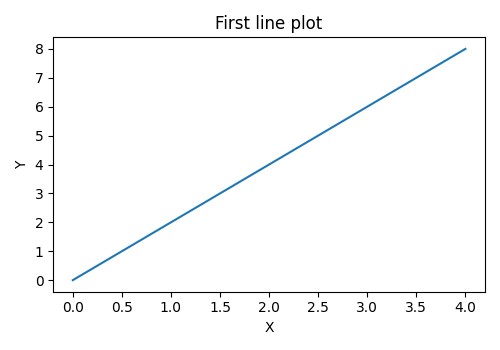
\includegraphics[width=0.6\linewidth]{Figures/Visualization/16.4.png}
    \caption{Simple line plot}
    \label{fig:lineplot}
\end{figure}

\hhh{Adding meaning: labels and titles}

A plot without labels is like a drawing without dimensions—it might look clean, but it fails to communicate meaningful information. In architectural practice, every drawing includes a title, scale, and labeled dimensions; the same applies to data visualization. Labels turn raw geometry into understandable information.

\textbf{Figure~\ref{fig:Adding_label_title}} shows how adding titles, axis labels, and grid lines transforms a basic line plot into a communicative diagram. 

Labels serve multiple purposes: they tell the viewer what each axis represents, specify measurement units, and provide context for interpretation. In architecture, failing to label units (meters vs.\ feet) can lead to catastrophic design errors—the same principle applies to visualized data.

\code{c16_plot_with_labels}{python}{
    import matplotlib.pyplot as plt
    
    # Let's plot something architectural: floor heights
    floors = [0, 1, 2, 3, 4, 5]  # Floor numbers
    heights = [0, 3.5, 7.0, 10.5, 14.0, 17.5]  # Height in meters
    
    # Create the plot
    plt.plot(floors, heights, marker='o')  # 'o' adds circles at each point
    
    # Add essential labels
    plt.xlabel('Floor Number')  # What's on the x-axis
    plt.ylabel('Height Above Ground (m)')  # What's on the y-axis (with units!)
    plt.title('Building Section: Floor Heights')  # What the plot shows
    
    # Add a grid for easier reading (like graph paper)
    plt.grid(True, alpha=0.3)  # alpha makes it subtle (30% opacity)
    
    # Display the plot
    plt.show()
    
    # Outcome (what you'll see):
    # A line plot with:
    # - Title: "Building Section: Floor Heights"
    # - X-axis: "Floor Number" (0–5)
    # - Y-axis: "Height Above Ground (m)" (0–17.5)
    # - Blue line connecting points with circular markers
    # - Subtle gray grid lines in background
    # - Clearly shows consistent 3.5 m floor-to-floor height
}{Adding essential labels to make the plot meaningful.}

\begin{figure}[htp!]
    \centering
    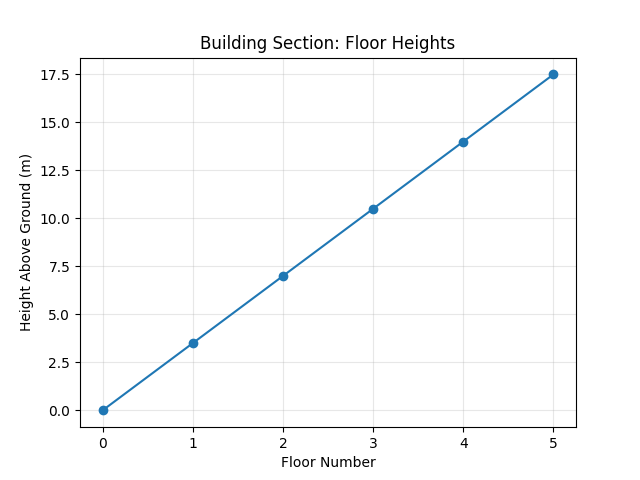
\includegraphics[width=0.6\linewidth]{Figures/Visualization/16.4.1.png}
    \caption{Enhancing meaning through titles and labels. The figure shows a simple line plot of floor heights in a six-story building. The title provides context (“Building Section: Floor Heights”), axis labels identify variables and units, and grid lines improve legibility—transforming a raw line into a readable architectural data graphic.}
    \label{fig:Adding_label_title}
\end{figure}


\hh{Basic syntax and line properties}

Before we layer on annotations and multiple axes, it helps to see how the core line properties work. The code below draws four small panels to illustrate \emph{line style} (\texttt{linestyle}), \emph{thickness} (\texttt{linewidth}), \emph{color} (\texttt{color}), and \emph{transparency} (\texttt{alpha}) shown in Figure \ref{fig:line_properties}. These are the building blocks you’ll reuse in every line plot.

\code{c16_plot_syntax_lines}{python}{
    import math
    import matplotlib.pyplot as plt

    # Build x as 50 points from 0 to 10 without NumPy
    x = [i * 10.0 / 49 for i in range(50)]
    y1 = [math.sin(v) for v in x]
    y2 = [math.cos(v) for v in x]
    y3 = [math.sin(v) * math.exp(-v / 10.0) for v in x]

    fig, axes = plt.subplots(2, 2, figsize=(12, 10))

    # SUBPLOT 1: Line styles (linestyle: '-', '--', '-.', ':')
    axes[0, 0].plot(x, y1, linestyle='-',  label='solid')
    axes[0, 0].plot(x, [yy - 0.5 for yy in y1], linestyle='--', label='dashed')
    axes[0, 0].plot(x, [yy - 1.0 for yy in y1], linestyle='-.', label='dash-dot')
    axes[0, 0].plot(x, [yy - 1.5 for yy in y1], linestyle=':',  label='dotted')
    axes[0, 0].set_title('Line styles')
    axes[0, 0].legend()
    axes[0, 0].grid(True, alpha=0.3)

    # SUBPLOT 2: Line widths (linewidth in points)
    axes[0, 1].plot(x, y1,                      linewidth=1, label='lw=1')
    axes[0, 1].plot(x, [yy - 0.5 for yy in y1], linewidth=2, label='lw=2')
    axes[0, 1].plot(x, [yy - 1.0 for yy in y1], linewidth=4, label='lw=4')
    axes[0, 1].plot(x, [yy - 1.5 for yy in y1], linewidth=6, label='lw=6')
    axes[0, 1].set_title('Line widths')
    axes[0, 1].legend()
    axes[0, 1].grid(True, alpha=0.3)

    # SUBPLOT 3: Colors (named, hex, RGB tuple, color cycle)
    axes[1, 0].plot(x, y1,                      color='red',        label='named')
    axes[1, 0].plot(x, [yy - 0.5 for yy in y1], color='#2E86AB',    label='hex')
    axes[1, 0].plot(x, [yy - 1.0 for yy in y1], color=(0.2, 0.7, 0.3), label='RGB tuple')
    axes[1, 0].plot(x, [yy - 1.5 for yy in y1], color='C2',         label='cycle C2')
    axes[1, 0].set_title('Color specifications')
    axes[1, 0].legend()
    axes[1, 0].grid(True, alpha=0.3)

    # SUBPLOT 4: Transparency (alpha in [0, 1])
    axes[1, 1].plot(x, y1, linewidth=3, alpha=1.0, label='alpha=1.0')
    axes[1, 1].plot(x, y2, linewidth=3, alpha=0.7, label='alpha=0.7')
    axes[1, 1].plot(x, y3, linewidth=3, alpha=0.4, label='alpha=0.4')
    axes[1, 1].set_title('Transparency control')
    axes[1, 1].legend()
    axes[1, 1].grid(True, alpha=0.3)

    plt.tight_layout()
    plt.show()
}{Line properties: styles, widths, colors, transparency.}

\begin{figure}
    \centering
    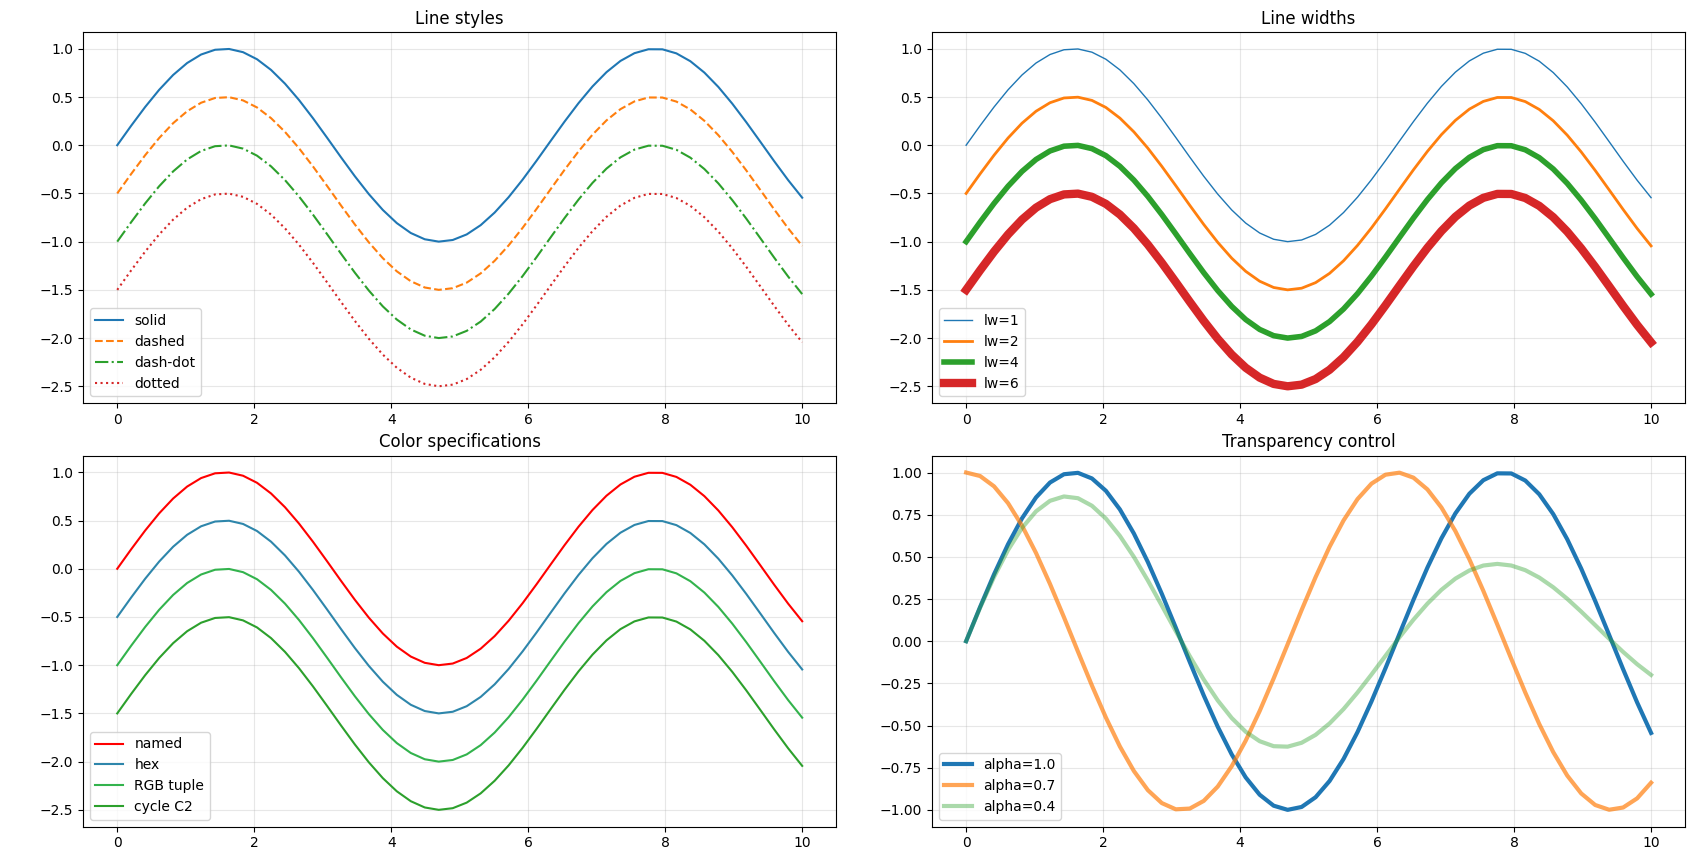
\includegraphics[width=1.0\linewidth]{Figures/Visualization/16.5.png}
    \caption{Line property essentials. Top-left: \emph{linestyle} variants; top-right: increasing \emph{linewidth}; bottom-left: different \emph{color} specifications (named, hex, RGB tuple, palette cycle); bottom-right: \emph{alpha} transparency.}
    \label{fig:line_properties}
\end{figure}


\hhh{How subplots and indexing work}

\textbf{\texttt{fig, axes = plt.subplots(nrows, ncols, ...)} returns:}
\begin{itemize}
  \item \texttt{fig}: the Figure (the whole page/canvas).
  \item \texttt{axes}: a grid (array) of \texttt{Axes} objects with shape \texttt{(nrows, ncols)}.
        Each cell is one plotting area.
\end{itemize}

\textbf{Zero-based indexing.} For a 2$\times$2 grid:
\[
\begin{array}{cc}
\texttt{axes[0, 0]}~(\text{top-left}) & \texttt{axes[0, 1]}~(\text{top-right}) \\
\texttt{axes[1, 0]}~(\text{bottom-left}) & \texttt{axes[1, 1]}~(\text{bottom-right})
\end{array}
\]

\begin{tcolorbox}[title=Subplot tips (quick reference), colframe=blue, colback=white, arc=2mm, breakable]
\begin{itemize}
  \item \textbf{Create grids:} \texttt{plt.subplots(2, 2, figsize=(12, 10))}.
  \item \textbf{Share axes (optional):} \texttt{sharex='col'}, \texttt{sharey='row'} (or \texttt{True} for all).
  \item \textbf{Tight spacing:} call \texttt{plt.tight\_layout()} or create with \texttt{constrained\_layout=True}.
  \item \textbf{Global title:} \texttt{fig.suptitle("Title")}.
  \item \textbf{Always 2D indexing (even 1x1):} use \texttt{squeeze=False} so you can write \texttt{axes[0, 0]}.
  \item \textbf{Loop over all panels:} \texttt{for ax in (ax for row in axes for ax in row): ...}
  \item \textbf{Manual spacing:} \texttt{fig.subplots\_adjust(wspace=..., hspace=...)}.
\end{itemize}
\end{tcolorbox}

When you create multi-panel figures, each panel is an \emph{Axes} object in a 2D array returned by \texttt{plt.subplots(rows, cols)}. You access panels with zero-based indices like \texttt{axes[0, 1]} (row 0, column 1). \textbf{Figure~\ref{fig:subplot_indexing}} shows four common customizations—line style, color, markers, and transparency—laid out in a \texttt{2$\times$2} grid. Note how \texttt{sharex='col'} synchronizes the x-axis within each column, and how we loop over the grid to place small index labels inside every panel. A \texttt{suptitle} provides a title for the whole figure, while \texttt{tight\_layout()} helps avoid label overlap.

\code{c16_subplot_indexing}{python}{
    import math
    import matplotlib.pyplot as plt

    # Build x without NumPy: 0..10 in 50 steps
    x = [i * 10.0 / 49 for i in range(50)]
    s = [math.sin(v) for v in x]
    c = [math.cos(v) for v in x]
    d = [s[i] - 0.5 for i in range(len(s))]  # shifted series

    # Create a 2x2 grid of subplots; share x within columns as an example
    fig, axes = plt.subplots(2, 2, figsize=(12, 8), sharex='col', sharey=False)

    # Top-left: line styles
    axes[0, 0].plot(x, s, linestyle='-',  label='solid')
    axes[0, 0].plot(x, d, linestyle='--', label='dashed')
    axes[0, 0].set_title("axes[0, 0]  (top-left)  --  line styles")
    axes[0, 0].legend(); axes[0, 0].grid(True, alpha=0.3)

    # Top-right: colors
    axes[0, 1].plot(x, s, color='C0', label='C0')
    axes[0, 1].plot(x, d, color='#2E86AB', label='#2E86AB')
    axes[0, 1].set_title("axes[0, 1]  (top-right)  --  colors")
    axes[0, 1].legend(); axes[0, 1].grid(True, alpha=0.3)

    # Bottom-left: markers
    axes[1, 0].plot(x, s, 'o-',  markersize=4, label="o-")
    axes[1, 0].plot(x, d, 's--', markersize=6, label="s--")
    axes[1, 0].set_title("axes[1, 0]  (bottom-left)  --  markers")
    axes[1, 0].legend(); axes[1, 0].grid(True, alpha=0.3)
    axes[1, 0].set_xlabel("x"); axes[1, 0].set_ylabel("y")

    # Bottom-right: transparency and a global annotation of the index
    axes[1, 1].plot(x, s, linewidth=3, alpha=0.6, label='alpha=0.6')
    axes[1, 1].plot(x, c, linewidth=3, alpha=0.3, label='alpha=0.3')
    axes[1, 1].set_title("axes[1, 1]  (bottom-right)  --  transparency")
    axes[1, 1].legend(); axes[1, 1].grid(True, alpha=0.3)
    axes[1, 1].set_xlabel("x")

    # Add small labels inside each panel showing its index
    for i in range(2):
        for j in range(2):
            axes[i, j].text(0.02, 0.92, f"axes[{i}, {j}]",
                            transform=axes[i, j].transAxes,
                            fontsize=9, bbox=dict(boxstyle="round,pad=0.2", fc="w", ec="0.7"))

    fig.suptitle("Subplot grid and axes indexing", fontsize=14, fontweight="bold")
    plt.tight_layout(); plt.show()
}{How to index and loop over a 2x2 subplot grid.}

\begin{figure}[htp!]
    \centering
    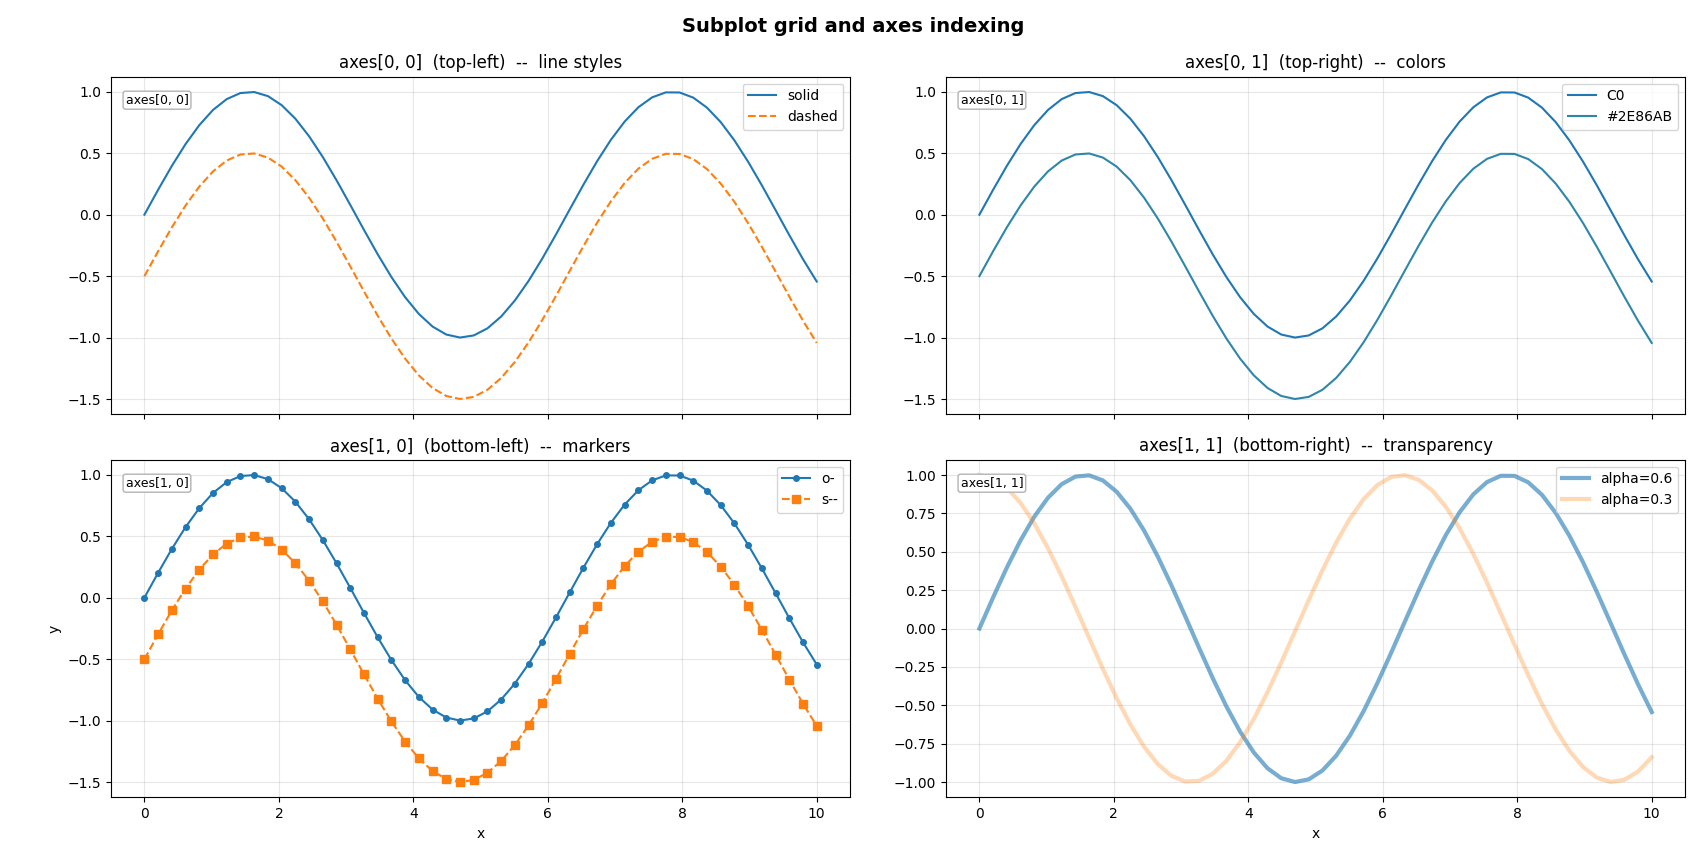
\includegraphics[width=1.0\linewidth]{Figures/Visualization/16.5.1.png}
    \caption{Subplot organization and indexing. Each panel is addressed by zero-based indices \(\texttt{axes[i, j]}\): top-left shows line styles, top-right color choices, bottom-left markers, and bottom-right transparency (\(\alpha\)). The figure uses \(\texttt{sharex='col'}\) to share x-axes within columns, a global \texttt{suptitle}, and a loop to annotate each panel with its \(\texttt{[i, j]}\) index.}
    \label{fig:subplot_indexing}
\end{figure}

\hhh{Marker properties}

Markers make individual data points visible along a line—crucial when you’re dealing with discrete measurements, sparse samples, or overlapping series. They also provide an additional visual channel (shape/size/fill/edge) to encode categories or emphasis without changing the line itself. \textbf{Figure~\ref{fig:marker_properties}} summarizes the essentials: common marker shapes, how size affects legibility, how to style filled vs.\ hollow markers, and how to combine format strings with explicit keyword arguments.

\code{c16_plot_syntax_markers}{python}{
    import math
    import matplotlib.pyplot as plt

    # 20 points from 0 to 10
    x = [i * 10.0 / 19 for i in range(20)]
    y = [math.sin(v) for v in x]

    fig, axes = plt.subplots(2, 2, figsize=(12, 10))

    # SUBPLOT 1: Marker styles
    markers = ['o', 's', '^', 'D', 'v', 'p', '*', 'h']
    for i, m in enumerate(markers):
        axes[0, 0].plot(x, [yy - i*0.3 for yy in y],
                        marker=m, markersize=8, linewidth=1, label=f"'{m}'")
    axes[0, 0].set_title('Common marker styles')
    axes[0, 0].legend(ncol=2, fontsize=9)
    axes[0, 0].grid(True, alpha=0.3)

    # SUBPLOT 2: Marker sizes
    sizes = [4, 8, 12, 16]
    for i, s in enumerate(sizes):
        axes[0, 1].plot(x, [yy - i*0.6 for yy in y],
                        marker='o', markersize=s, linewidth=2,
                        label=f'markersize={s}')
    axes[0, 1].set_title('Marker sizes'); axes[0, 1].legend(); axes[0, 1].grid(True, alpha=0.3)

    # SUBPLOT 3: Marker face/edge
    axes[1, 0].plot(x, y, marker='o', markersize=10,
                    markerfacecolor='red', markeredgecolor='black',
                    markeredgewidth=2, label='filled with edge')
    axes[1, 0].plot(x, [yy - 0.5 for yy in y], marker='s', markersize=10,
                    markerfacecolor='none', markeredgecolor='blue',
                    markeredgewidth=2, label='hollow with edge')
    axes[1, 0].set_title('Marker fill and edges'); axes[1, 0].legend(); axes[1, 0].grid(True, alpha=0.3)

    # SUBPLOT 4: Combining line and marker options
    axes[1, 1].plot(x, y, 'ro-', markersize=8, linewidth=2, label="format string: 'ro-'")
    axes[1, 1].plot(x, [yy - 0.5 for yy in y], marker='s', color='blue',
                    linestyle='--', markersize=8, linewidth=2, label='keywords')
    axes[1, 1].set_title('Combining properties'); axes[1, 1].legend(); axes[1, 1].grid(True, alpha=0.3)

    plt.tight_layout(); plt.show()
}{Marker styles, sizes, colors, and edges.}

\begin{figure}[htp!]
    \centering
    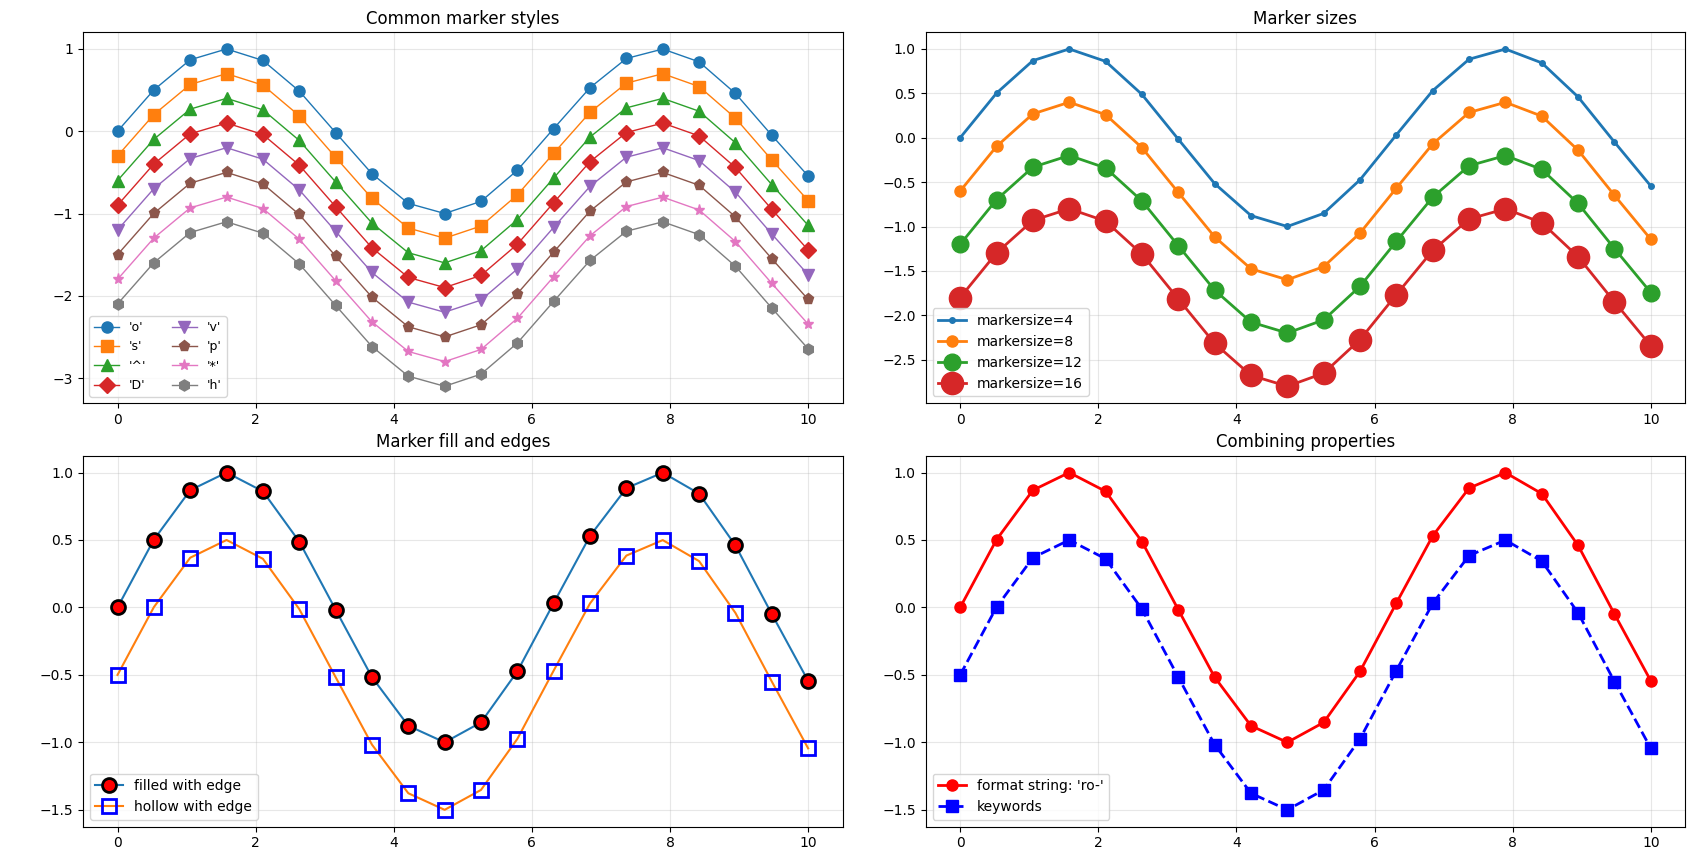
\includegraphics[width=1.0\linewidth]{Figures/Visualization/16.5.2.png}
    \caption{Marker property overview. Top-left: common marker shapes (\texttt{'o'}, \texttt{'s'}, \texttt{'$\wedge$'}, \texttt{'D'}, \texttt{'v'}, \texttt{'p'}, \texttt{'*'}, \texttt{'h'}). Top-right: the impact of \texttt{markersize} on legibility. Bottom-left: filled vs.\ hollow markers using \texttt{markerfacecolor}/\texttt{markeredgecolor}/\texttt{markeredgewidth}. Bottom-right: combining a format string (e.g., \texttt{'ro-'}) with explicit keyword styling.}
    \label{fig:marker_properties}
\end{figure}

As shown in Figure~\ref{fig:marker_properties}, choose marker shapes for categorical distinction, size for visibility at your final figure dimensions, and face/edge settings to maintain contrast on light or dark lines/backgrounds.


\hhh{Format strings: quick specification}

Matplotlib supports compact \emph{format strings} that combine color, marker, and line style in a single shorthand argument. This is the quickest way to specify common style combinations when prototyping or creating simple visualizations. Each format string follows the pattern:

\[
[\text{color}][\text{marker}][\text{linestyle}]
\]

where all components are optional.  
For example, \texttt{'r--'} means a red dashed line, \texttt{'bo-'} means blue circles connected by a solid line, and \texttt{'kD'} means black diamond markers with no connecting line.

Figure~\ref{fig:format_string} demonstrates several format strings at once, showing how a single short code defines multiple visual attributes—useful for concise and readable plotting commands.

\code{c16_plot_format_strings}{python}{
    import math
    import matplotlib.pyplot as plt

    x = [i * 10.0 / 14 for i in range(15)]
    y = [math.sin(v) for v in x]

    fig, ax = plt.subplots(figsize=(10, 6))

    # Format string syntax: [color][marker][linestyle]
    ax.plot(x, y,       'r-',   label="'r-' = red solid line")
    ax.plot(x, [yy-0.5 for yy in y], 'bs--', label="'bs--' = blue squares, dashed")
    ax.plot(x, [yy-1.0 for yy in y], 'g^:',  label="'g^:' = green triangles, dotted")
    ax.plot(x, [yy-1.5 for yy in y], 'mo-.', label="'mo-.' = magenta circles, dash-dot")
    ax.plot(x, [yy-2.0 for yy in y], 'kD',   label="'kD' = black diamonds, no line")

    ax.set_title('Format string examples: [color][marker][linestyle]', fontsize=14, fontweight='bold')
    ax.set_xlabel('X axis'); ax.set_ylabel('Y axis')
    ax.legend(loc='upper right', fontsize=10)
    ax.grid(True, alpha=0.3)

    plt.tight_layout(); plt.show()

    # Common components (printed to console)
    print("COLOR CODES: b=blue, g=green, r=red, c=cyan,")
    print("             m=magenta, y=yellow, k=black, w=white")
    print("\\nMARKER CODES: o=circle, s=square, ^=triangle,")
    print("               D=diamond, *=star, +=plus, x=x-mark")
    print("\\nLINE CODES: '-'=solid, '--'=dashed, ':'=dotted, '-.'=dash-dot")
}{Format strings for quick plot styling.}

\begin{figure}[htp!]
    \centering
    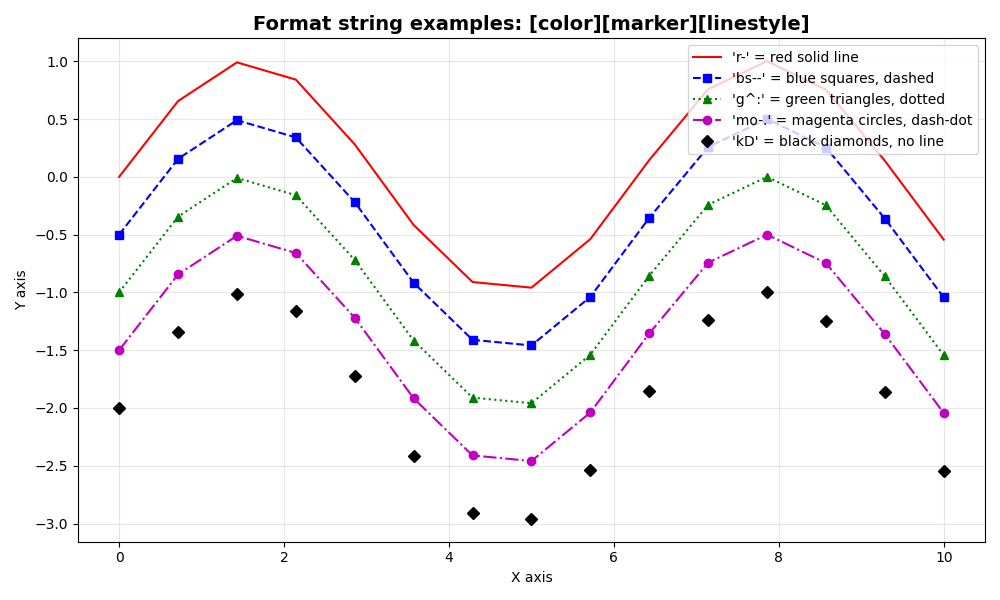
\includegraphics[width=0.75\linewidth]{Figures/Visualization/16.5.3.png}
    \caption{Examples of Matplotlib format strings combining color, marker, and line style. Each short code defines a complete visual combination: \texttt{'r-'} (red solid line), \texttt{'bs--'} (blue squares with dashed line), \texttt{'g\textasciicircum:'} (green triangles with dotted line), \texttt{'mo-.'} (magenta circles with dash-dot line), and \texttt{'kD'} (black diamonds without connecting line).}
    \label{fig:format_string}
\end{figure}


\hhh{Complete plot() parameter reference}
\begin{tcolorbox}[
    title=plot() function parameters,
    colframe=blue,
    colback=white,
    arc=2mm,
    breakable
]
\textbf{Call forms}\\
\texttt{plot(y)} (x is 0..N-1) \quad
\texttt{plot(x, y)} \quad
\texttt{plot(x, y1, x, y2, ...)} for multiple series.

\medskip
\textbf{Line properties}
\begin{itemize}
  \item \texttt{color} (or \texttt{c}): name, hex, or RGB(A) tuple.
  \item \texttt{linestyle} (or \texttt{ls}): \verb|-|, \verb|--|, \verb|-.|, \verb|:|, or \texttt{None}.
  \item \texttt{linewidth} (or \texttt{lw}): float width in points.
  \item \texttt{alpha}: transparency in [0, 1].
  \item \texttt{drawstyle}: step variants (for example, \texttt{steps-mid}).
\end{itemize}

\textbf{Marker properties}
\begin{itemize}
  \item \texttt{marker}: for example, \verb|o|, \verb|s|, \verb|^|, \verb|D|, \verb|*|, \verb|+|, \verb|x|.
  \item \texttt{markersize} (or \texttt{ms}): float.
  \item \texttt{markerfacecolor} (or \texttt{mfc}), \texttt{markeredgecolor} (or \texttt{mec}).
  \item \texttt{markeredgewidth} (or \texttt{mew}).
  \item \texttt{markevery}: int or tuple to thin markers (for example, \texttt{markevery=5}).
\end{itemize}

\textbf{Labels and z-order}
\begin{itemize}
  \item \texttt{label}: legend text.
  \item \texttt{zorder}: draw order (larger draws on top).
  \item \texttt{visible}: True/False to show/hide.
\end{itemize}

\textbf{Axes helpers (common)}
\begin{itemize}
  \item Titles/labels: \texttt{ax.set\_title()}, \texttt{ax.set\_xlabel()}, \texttt{ax.set\_ylabel()}.
  \item Grid: \texttt{ax.grid(True, alpha=0.3)}.
  \item Legend: \texttt{ax.legend()} (uses \texttt{label=} from plots).
\end{itemize}
\end{tcolorbox}

% =====================
% PART II: ESSENTIAL PLOT TYPES FOR ARCHITECTURE
% =====================

\hh{Understanding when to use different plot types}

Choosing the right visualization type is like choosing the right drawing type in architecture. You wouldn't use a floor plan to show a building's height, and you shouldn't use a pie chart to show change over time. Each plot type has specific strengths and appropriate uses. Understanding these will help you communicate data effectively.

In architectural practice, we choose drawings based on what we need to communicate: plans show horizontal relationships, sections show vertical relationships, and perspectives show experiential qualities. Similarly, each plot type excels at showing different data relationships:

\begin{itemize}
\item \textbf{Bar charts}: Compare quantities across categories (room areas, costs by trade)
\item \textbf{Line plots}: Show trends over time (energy use by month, construction schedule)
\item \textbf{Scatter plots}: Reveal correlations between variables (window area vs. daylight)
\item \textbf{Heat maps}: Display values across two dimensions (solar radiation on facade)
\item \textbf{Histograms}: Show distributions (distribution of apartment sizes in a building)
\item \textbf{Pie charts}: Show parts of a whole (program percentages)---use sparingly!
\end{itemize}

% =========================================================
% Matplotlib — Bar Charts (ARC500)
% Uses course macros: \h, \hh, \hhh, \code
% =========================================================

\hh{Bar charts}

Bar charts compare \emph{categories} (e.g., rooms, materials, cost items). They are ideal when categories are discrete and do not imply continuity. In architectural practice: space programs, cost breakdowns, material quantities, and headcounts are common use cases.

\textbf{Design tips.} (1) Start the value axis at zero for honest comparison, (2) label axes and units, (3) prefer sorting by value, (4) avoid excessive colors; reserve color to encode meaning, (5) use horizontal bars when labels are long.

\textbf{Bar chart vs. histogram.} A \emph{bar chart} compares categories; a \emph{histogram} shows frequency of numeric values across bins. They look similar but answer different questions.

\hhh{Core syntax (Matplotlib) — arguments and parameters}

\textbf{Vertical bars}
\begin{lstlisting}[language=Python, frame=single, backgroundcolor=\color{gray!5}]
    plt.bar(x, height, *, width=0.8, bottom=None, align='center',
            label=None, color=None, edgecolor=None, linewidth=None, alpha=None)
    # x: category positions. Can be numbers (0..N-1) or strings (e.g., room names).
    # height: bar heights (array-like: list, NumPy array, Pandas Series).
    # *: keyword-only separator — everything after this must be named (e.g., width=0.8).

    # width: thickness of each vertical bar (in "category" units). Smaller (<0.8) leaves gaps.
    # bottom: baseline (vertical offset) for each bar. Use for stacked bars or to shift negatives.
    # align: 'center' (default) centers bars on x; 'edge' aligns left edges at x.
    # label: series label for legends (ax.legend()).
    # color: fill — a single color or a list/array matching bars; accepts hex, named, RGBA.
    # edgecolor: border color for bars.
    # linewidth: width of bar borders.
    # alpha: transparency from 0 (transparent) to 1 (opaque).
\end{lstlisting}

\textbf{Horizontal bars}
\begin{lstlisting}[language=Python, frame=single, backgroundcolor=\color{gray!5}]
    plt.barh(y, width, *, height=0.8, left=None, align='center', **kwargs)
    # y: categories on the vertical axis (numbers or strings).
    # width: bar lengths along the horizontal axis (array-like).

    # height: thickness of each horizontal bar (category units).
    # left: baseline (horizontal offset) for each bar; use for stacking or shifting.
    # align: 'center' (default) centers bars on y; 'edge' aligns bottom edges at y.
    # **kwargs: forwarded to the underlying Rectangle artists (e.g., color, edgecolor, alpha, label).
\end{lstlisting}

\textbf{Practical notes}
\begin{itemize}
    \item \textbf{Categorical ticks.} If \texttt{x} (or \texttt{y} for \texttt{barh}) is a list of strings, Matplotlib handles tick placement/labels automatically. With numeric positions, set labels via \texttt{ax.set\_xticks/xticklabels}.
    \item \textbf{Stacked bars.} Pass \texttt{bottom=} (or \texttt{left=} for \texttt{barh}) as the cumulative sum of previous series to stack values.
    \item \textbf{Multiple series (grouped).} Offset numeric positions: \texttt{x - w/2}, \texttt{x + w/2}, etc., where \texttt{w} is the bar \texttt{width}.
    \item \textbf{Negative values.} Bars extend below the baseline. Use \texttt{bottom} (or \texttt{left}) to shift the zero line if needed and add a reference line with \texttt{ax.axhline(0,...)} or \texttt{ax.axvline(0,...)}.
    \item \textbf{Color control.} A single \texttt{color='...'} applies to all bars; a list/array assigns per-bar colors. Combine with \texttt{edgecolor} and \texttt{linewidth} for clarity.
    \item \textbf{Annotation.} Use \texttt{ax.text(x, y, "...")} to place value labels; for \texttt{barh}, swap axes accordingly.
    \item \textbf{Layout.} Finish with \texttt{plt.tight\_layout()} before \texttt{plt.show()} to avoid label clipping.
\end{itemize}


\textbf{Axes helpers (frequently used)}
\begin{lstlisting}[language=Python, frame=single, backgroundcolor=\color{gray!5}]
    # Titles and axis labels
    ax.set_title("Figure title", loc='center', pad=6)
    # loc: 'left' | 'center' | 'right'; pad: extra points above the title
    ax.set_xlabel("X label", labelpad=4)
    ax.set_ylabel("Y label", labelpad=4)
    # labelpad adds spacing between label and axis

    # Tick labels (categorical or rotated labels)
    ax.set_xticklabels(labels, rotation=0, ha='center')
    # labels: list of strings (use with existing tick positions)
    # rotation: degrees (e.g., 30, 45, 90); ha: 'left' | 'center' | 'right'

    # Grid lines (helps reading bar values)
    ax.grid(True, axis='x', linestyle=':', linewidth=0.8, alpha=0.3)
    # axis: 'x' for vertical bars, 'y' for horizontal bars
    # linestyle: '-', '--', ':', '-.'; alpha: transparency

    # Reference/benchmark line (e.g., average)
    ax.axhline(y=value, xmin=0.0, xmax=1.0, linestyle='--', color='C3', label='Benchmark')
    # y: y-coordinate for horizontal line; xmin/xmax in axes fraction [0..1]

    # Annotate (place text near a bar)
    ax.text(x, y, "label", ha='center', va='bottom', rotation=0)
    # x, y in data coordinates; ha/va: text alignment; rotation in degrees

    # Legend and layout
    ax.legend(loc='best', frameon=False)
    plt.tight_layout()   # prevent label/title clipping
    plt.show()
\end{lstlisting}

\textit{Notes.}
\begin{itemize}
    \item \textbf{Ticks for categories.} If you created bars with string categories (e.g., \texttt{plt.bar(['A','B'], ...)}), Matplotlib sets ticks automatically. If you used numeric positions (e.g., \texttt{x = np.arange(N)}), pair with \texttt{ax.set\_xticks(x)} and \texttt{ax.set\_xticklabels(labels)}.
    \item \textbf{Rotation for long labels.} Use \texttt{rotation=30} or \texttt{45} and optionally \texttt{ha='right'} plus \texttt{plt.tight\_layout()} to avoid overlap.
    \item \textbf{Grid direction.} For vertical bar charts, readers compare \emph{heights}—so enable \texttt{axis='y'} if you want horizontal grid lines; use \texttt{axis='x'} when you prefer vertical reference lines. For \texttt{barh}, swap accordingly.
    \item \textbf{Benchmark lines.} Use \texttt{ax.axhline} for vertical bars (average/target). For horizontal bars, use \texttt{ax.axvline(x=...)} instead.
    \item \textbf{Text placement.} For labels above bars, set \texttt{y = bar\_height + offset} and \texttt{va='bottom'}. For \texttt{barh}, place at \texttt{x = bar\_length + offset} and \texttt{ha='left'}.
    \item \textbf{Legends.} Provide \texttt{label=} in plotting calls (e.g., bars, \texttt{axhline}) so \texttt{ax.legend()} has entries. \texttt{frameon=False} removes the legend box if you want a cleaner look.
\end{itemize}


\hhh{Bar chart: comparing room areas}

Bar charts are ideal for comparing discrete categories that have no natural continuous relationship—such as room areas, costs, or material quantities. Each bar represents one category, with its height corresponding to its value. In architectural visualization, this is equivalent to comparing space sizes in a program diagram.  

{Figure~\ref{fig:bargraph}} shows a simple vertical bar chart comparing room areas in a small apartment. A horizontal dashed line marks the average room size, and each bar is labeled with its numeric value for quick reference.

\code{c16_first_bar_chart}{python}{
    import matplotlib.pyplot as plt

    # Room data for a small apartment
    rooms = ['Living', 'Kitchen', 'Bedroom', 'Bathroom']
    areas = [25.5, 12.3, 16.8, 6.4]  # Areas in square meters

    # Create a bar chart
    plt.figure(figsize=(8, 6))

    # Bars (categorical x = room names, heights = areas)
    bars = plt.bar(rooms, areas, color='skyblue', edgecolor='navy', linewidth=1.5)

    # Labels and title
    plt.xlabel('Room')
    plt.ylabel('Area (m$^2$)')
    plt.title('Apartment Room Areas')

    # Add numeric labels on top of each bar
    for i, (room, area) in enumerate(zip(rooms, areas)):
        plt.text(i, area + 0.5, f'{area} m$^2$', ha='center', va='bottom')

    # Average line (visual benchmark)
    avg = sum(areas) / len(areas)
    plt.axhline(y=avg, color='red', linestyle='--', label=f'Average: {avg:.1f} m$^2$')
    plt.legend()

    plt.tight_layout()
    plt.show()

    # Quick stats (console)
    total = sum(areas)
    print(f"Total apartment area: {total} m$^2$")
    print(f"Average room area: {avg:.1f} m$^2$")
}{Creating a vertical bar chart to compare room areas.}

\begin{figure}[bhtp]
    \centering
    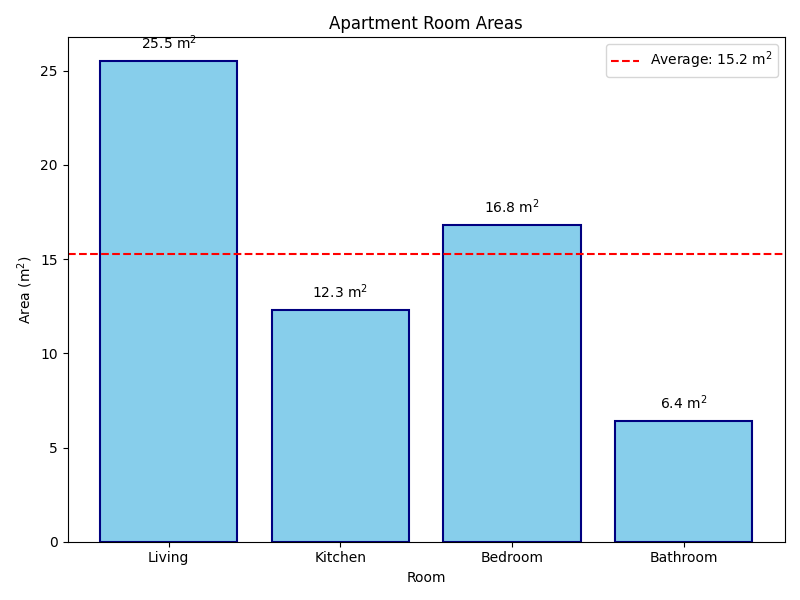
\includegraphics[width=0.6\linewidth]{Figures/Visualization/16.7.2.png}
    \caption{Vertical bar chart comparing room areas in a small apartment. Each bar represents a room, labeled with its area in square meters. A red dashed line indicates the average room size, helping identify which rooms are above or below average.}
    \label{fig:bargraph}
\end{figure}

\hhh{Distributions: histogram}

While bar charts compare categories, histograms reveal the distribution of continuous numeric data. Instead of individual categories, data are grouped into \emph{bins}, each showing how many observations fall within a range.  

In architecture, histograms help visualize the spread of room areas, energy use intensities, or daylight factors.  
{Figure~\ref{fig:histogram}} shows an example: a simulated distribution of apartment unit sizes centered around 55~m$^2$.

\code{viz_hist}{python}{
    import random
    import matplotlib.pyplot as plt

    # Fake unit sizes (m$^2$) around 55 with noise
    data = [55 + random.gauss(0, 10) for _ in range(400)]

    fig, ax = plt.subplots(figsize=(6, 3.5))
    ax.hist(data, bins=20, edgecolor='black')
    ax.set_title('Unit size distribution')
    ax.set_xlabel('Area (m$^2$)')
    ax.set_ylabel('Count')

    plt.tight_layout()
    plt.show()
}{Histogram with bins (distribution of numeric values).}

\begin{figure}[bhtp]
    \centering
    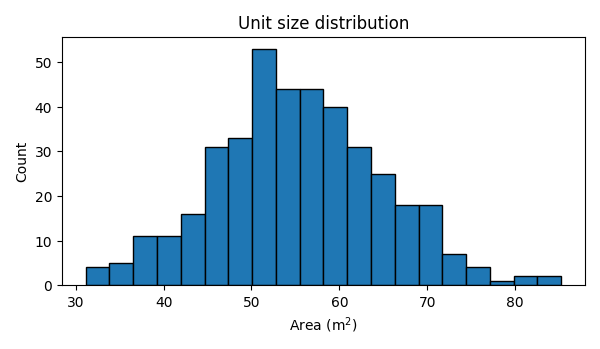
\includegraphics[width=0.6\linewidth]{Figures/Visualization/16.7.3.png}
    \caption{Histogram showing the distribution of apartment unit sizes. The x-axis represents area ranges, and the y-axis shows the count of units per range. The bell-shaped curve indicates that most units cluster near the 55~m$^2$ average, with fewer very small or very large units.}
    \label{fig:histogram}
\end{figure}

\hhh{Horizontal bars for long labels}

When category names are long or numerous—such as in a building program—horizontal bars improve readability and prevent label overlap. This format also leaves more space for text, annotations, or summaries.  

{Figure~\ref{fig:horizontalbar}} presents a medical clinic program with spaces sorted by area. Functional color coding distinguishes clinical, staff, support, and circulation zones, and a text box summarizes total and category areas.

\code{c16_horizontal_bars_detailed}{python}{
    import matplotlib.pyplot as plt

    # Medical clinic space program (m$^2$)
    spaces = {
        'Waiting Room': 45, 'Reception/Check-in': 25,
        'Exam Room 1': 15, 'Exam Room 2': 15, 'Exam Room 3': 15,
        'Procedure Room': 25, "Doctor's Office": 12, 'Nurse Station': 18,
        'Medical Storage': 10, 'Staff Break Room': 12,
        'Accessible Restroom': 8, 'Standard Restroom': 6,
        'Utility/Janitor': 6, 'Circulation/Corridor': 48,
    }

    # Sort by area (ascending)
    rooms, areas = zip(*sorted(spaces.items(), key=lambda kv: kv[1]))

    fig, ax = plt.subplots(figsize=(10, 8))
    bars = ax.barh(rooms, areas)

    # Simple, meaningful color logic (optional)
    for b, name in zip(bars, rooms):
        if 'Exam' in name or 'Procedure' in name:
            b.set_color('#4CAF50')     # clinical
        elif 'Office' in name or 'Nurse' in name or 'Break' in name:
            b.set_color('#2196F3')     # staff
        elif 'Storage' in name or 'Utility' in name:
            b.set_color('#9E9E9E')     # support
        elif 'Restroom' in name:
            b.set_color('#FF9800')     # restroom
        elif 'Circulation' in name:
            b.set_color('#795548')     # circulation
        else:
            b.set_color('#9C27B0')     # public

    # Edges for clarity
    for b in bars:
        b.set_edgecolor('black')
        b.set_linewidth(1)

    # Labels and title
    ax.set_xlabel('Area (m$^2$)')
    ax.set_ylabel('Space')
    ax.set_title('Medical Clinic Space Program — Sorted by Area', pad=14)

    # Value labels at bar ends
    for y, area in enumerate(areas):
        ax.text(area + 1, y, f'{area} m$^2$', va='center')

    # Light grid
    ax.grid(True, axis='x', alpha=0.3, linestyle=':')

    # Summary box
    total = sum(spaces.values())
    clinical = sum(v for k, v in spaces.items() if 'Exam' in k or 'Procedure' in k)
    circ_pct = spaces['Circulation/Corridor'] / total * 100
    summary = f'Total: {total} m$^2$\nClinical: {clinical} m$^2$\nCirculation: {circ_pct:.1f}%'
    ax.text(0.98, 0.02, summary, transform=ax.transAxes,
            ha='right', va='bottom',
            bbox=dict(boxstyle='round', facecolor='wheat', alpha=0.8))

    plt.tight_layout()
    plt.show()

    # Console analysis
    print("Space Analysis")
    print(f"Total area: {total} m$^2$")
    print(f"Clinical spaces: {clinical} m$^2$ ({clinical/total*100:.1f}%)")
    print(f"Average room size: {total/len(spaces):.1f} m$^2$")
    print(f"Largest: {max(spaces, key=spaces.get)} ({max(spaces.values())} m$^2$)")
    print(f"Smallest: {min(spaces, key=spaces.get)} ({min(spaces.values())} m$^2$)")
}{Horizontal bar chart with sorting, color coding, labels, and summary box.}

\begin{figure}[bhtp]
    \centering
    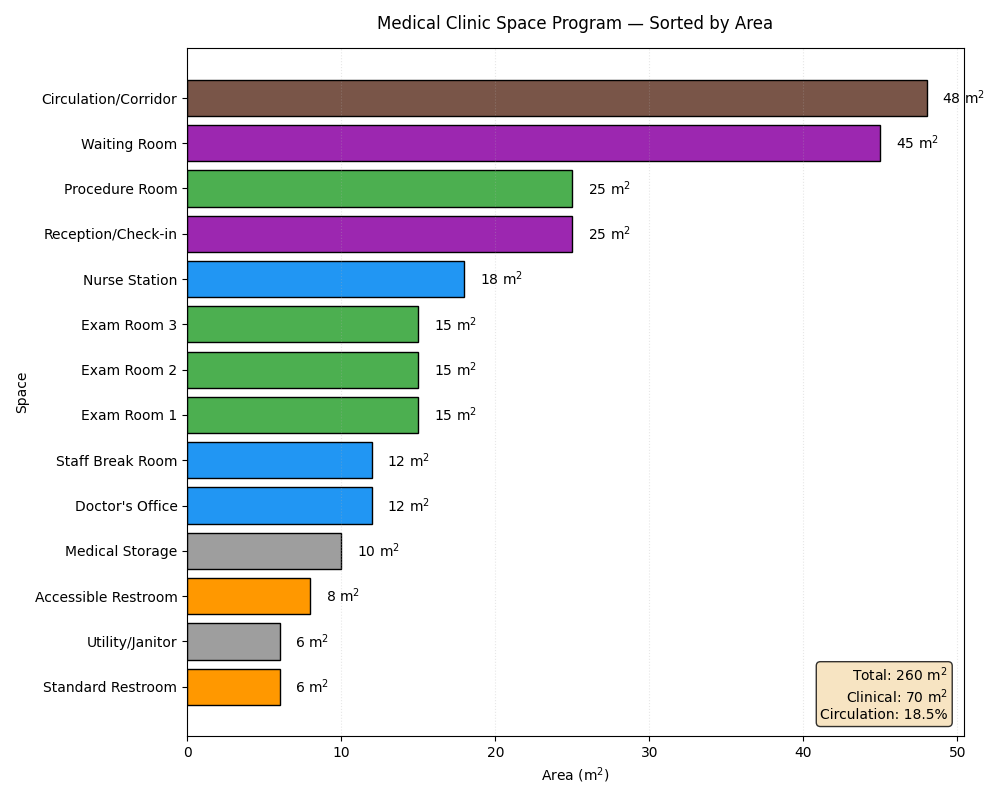
\includegraphics[width=0.8\linewidth]{Figures/Visualization/16.7.4.png}
    \caption{Horizontal bar chart of a medical clinic space program, sorted by area. Color coding differentiates space types: green for clinical, blue for staff, gray for support, orange for restrooms, and brown for circulation. Labels and a summary box enhance clarity and readability.}
    \label{fig:horizontalbar}
\end{figure}


\hhh{Grouped and stacked bars}

\textbf{Grouped bars} compare multiple series across the same categories (e.g., existing vs.\ proposed areas). 
As shown in {Figure~\ref{fig:grouped_bars}}, each category (Lobby, Office, Lab) has two adjacent bars so you can compare series side-by-side.

\code{c16_grouped_bars}{python}{
    import numpy as np
    import matplotlib.pyplot as plt

    cats = ['Lobby','Office','Lab']
    existing = [40, 60, 30]; proposed = [45, 55, 42]
    x = np.arange(len(cats)); w = 0.35

    fig, ax = plt.subplots()
    ax.bar(x - w/2, existing, width=w, label='Existing')
    ax.bar(x + w/2, proposed, width=w, label='Proposed')
    ax.set_xticks(x); ax.set_xticklabels(cats)
    ax.set_ylabel('Area (m$^2$)')
    ax.legend()
    plt.tight_layout(); plt.show()
}{Grouped bars: side-by-side comparison across categories.}

% (Add your figure here)
\begin{figure}
     \centering
     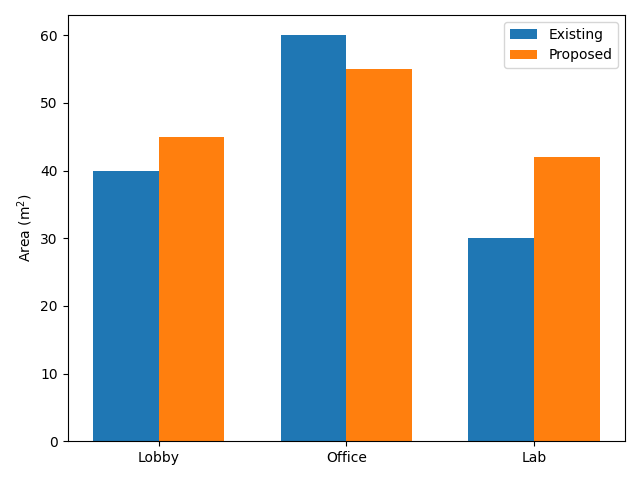
\includegraphics[width=0.6\linewidth]{Figures/Visualization/16.7.5.png}
     \caption{Grouped bar chart comparing \emph{Existing} vs.\ \emph{Proposed} areas for Lobby, Office, and Lab. Bars are placed side-by-side within each category to support quick comparison of the two series.}
     \label{fig:grouped_bars}
 \end{figure}

\medskip

\textbf{Stacked bars} show composition within each category by stacking series vertically so the bar height equals the total. This is useful when you care about both the overall magnitude and how it breaks down. As shown in {Figure~\ref{fig:stacked_bars}}, each category’s bar stacks \emph{Core} underneath \emph{Usable}. To avoid any ambiguity in stacking, we use numeric x-positions and explicit \texttt{bottom=} arrays.

\code{c16_stacked_bars}{python}{
    import numpy as np
    import matplotlib.pyplot as plt

    cats = ['Lobby','Office','Lab']
    core = np.array([15, 18, 12], dtype=float)
    usable = np.array([25, 32, 20], dtype=float)

    x = np.arange(len(cats))
    width = 0.6  # a bit wider for readability

    fig, ax = plt.subplots(figsize=(7, 4.5))

    # Base layer
    p1 = ax.bar(x, core, width=width, label='Core', edgecolor='black')

    # Stacked layer (explicit bottom = core)
    p2 = ax.bar(x, usable, width=width, bottom=core, label='Usable', edgecolor='black')

    # Axis + ticks
    ax.set_xticks(x)
    ax.set_xticklabels(cats)
    ax.set_ylabel('Area (m$^2$)')
    ax.set_title('Stacked bar chart: Core + Usable')

    # Optional totals on top
    totals = core + usable
    for xi, tot in zip(x, totals):
        ax.text(xi, tot + 1, f'{tot:.0f}', ha='center', va='bottom', fontsize=9)

    ax.legend()
    ax.grid(True, axis='y', alpha=0.25, linestyle=':')
    plt.tight_layout(); plt.show()
}{Stacked bars: show totals and composition per category.}

% (Add your figure file here)
\begin{figure}
     \centering
     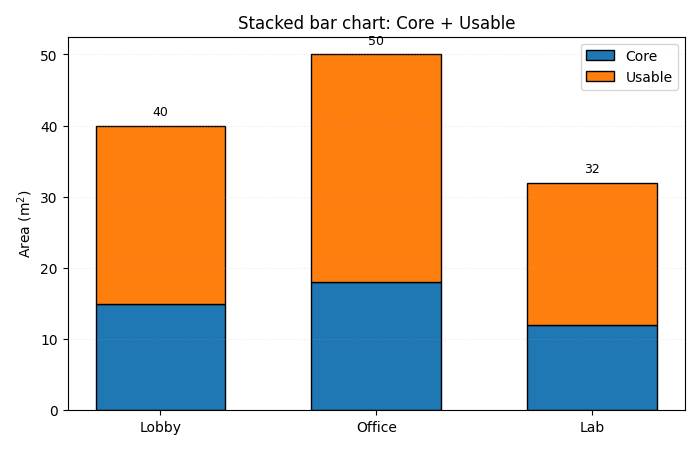
\includegraphics[width=0.6\linewidth]{Figures/Visualization/16.7.5b.png}
     \caption{Stacked bar chart showing category composition. Each bar’s height equals the total area (Core + Usable). Labels on top indicate totals, while color segments reveal the internal breakdown.}
     \label{fig:stacked_bars}
\end{figure}

\medskip

Sometimes relative composition matters more than absolute totals. {Figure~\ref{fig:stacked_bars_pct}} shows a 100\% stacked view, where each bar spans 0–100\% and segments indicate the share of each component.

\code{c16_stacked_bars_pct}{python}{
    import numpy as np
    import matplotlib.pyplot as plt

    cats = ['Lobby','Office','Lab']
    core = np.array([15, 18, 12], dtype=float)
    usable = np.array([25, 32, 20], dtype=float)

    totals = core + usable
    core_pct = core / totals * 100.0
    usable_pct = usable / totals * 100.0

    x = np.arange(len(cats))
    width = 0.6

    fig, ax = plt.subplots(figsize=(7, 4.5))
    ax.bar(x, core_pct,   width=width, label='Core',   edgecolor='black')
    ax.bar(x, usable_pct, width=width, bottom=core_pct, label='Usable', edgecolor='black')

    ax.set_xticks(x)
    ax.set_xticklabels(cats)
    ax.set_ylim(0, 100)
    ax.set_ylabel('Share (%)')
    ax.set_title('100% stacked bar chart: share of Core vs. Usable')

    # Optional inside-percentage labels
    for xi, cp, up in zip(x, core_pct, usable_pct):
        ax.text(xi, cp/2, f'{cp:.0f}%', ha='center', va='center', fontsize=9)
        ax.text(xi, cp + up/2, f'{up:.0f}%', ha='center', va='center', fontsize=9)

    ax.legend(loc='upper right')
    ax.grid(True, axis='y', alpha=0.25, linestyle=':')
    plt.tight_layout(); plt.show()
}{100\% stacked bars: emphasize relative composition.}

% (Add your figure file here)
\begin{figure}
     \centering
     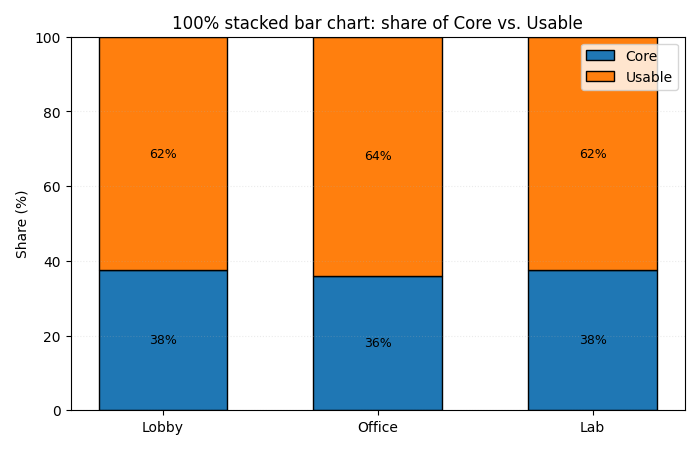
\includegraphics[width=0.6\linewidth]{Figures/Visualization/16.7.5c.png}
     \caption{100\% stacked bar chart where each category spans 0–100\%. Segment heights encode the share of Core and Usable, making relative composition immediately comparable across categories.}
     \label{fig:stacked_bars_pct}
\end{figure}


% (Add your figure here)
% \begin{figure}
%     \centering
%     \includegraphics[width=0.8\linewidth]{Figures/Visualization/<your-file>.png}
%     \caption{Stacked bar chart showing category composition: \emph{Core} (base segment) and \emph{Usable} (stacked segment) for Lobby, Office, and Lab. This view emphasizes both the total height (overall area) and the internal breakdown.}
%     \label{fig:stacked_bars}
% \end{figure}


\hhh{Common pitfalls and checklist}

\begin{itemize}
    \item \textbf{Start at zero} on the value axis; truncated axes can mislead.
    \item \textbf{Sort categories} when order is arbitrary to reveal patterns.
    \item \textbf{Use horizontal bars} for long labels.
    \item \textbf{Annotate} key values (totals, averages) to reduce table-lookups.
    \item \textbf{Minimize colors}; use color to encode meaning (type/function), not decoration.
    \item \textbf{Legibility}: readable fonts, sufficient figure size, notches between groups.
\end{itemize}


\hh{Line plots}

Line plots show how a quantity varies with a continuous variable (most commonly \emph{time}). In architectural contexts they are useful for energy profiles, temperature curves, construction schedules, and occupancy patterns. Unlike bars, a line implies continuity between points and makes trends and turning points apparent. Multiple lines allow scenario or system comparisons on the same axes.

\hhh{Core syntax — arguments and parameters}

\code{c16_line_core_syntax}{python}{
    # High-level calls (stateful and OO). Prefer the OO (ax.plot) form in multi-axes figures.
    plt.plot(x, y, fmt='', *, linewidth=None, linestyle=None, marker=None,
             color=None, label=None, alpha=None, markersize=None)

    fig, ax = plt.subplots()
    ax.plot(x, y, fmt='', *, linewidth=None, linestyle=None, marker=None,
            color=None, label=None, alpha=None, markersize=None)
}{Core line-plot calls and parameters}

\textbf{Arguments explained}
\begin{itemize}
    \item \texttt{x}: x-coordinates (array-like). Can be numbers, strings (categorical months like \texttt{["Jan", ...]}), or datetimes (e.g., \texttt{pd.DatetimeIndex}).
    \item \texttt{y}: y-values (array-like). Must match \texttt{x} in length.
    \item \texttt{fmt}: compact style string (optional) combining color/marker/linestyle (e.g., \texttt{'o--'}, \texttt{'r-.'}). Use explicit kwargs for clarity in reports.
\end{itemize}

\textbf{Common keyword parameters}
\begin{itemize}
    \item \texttt{linewidth} or \texttt{lw}: thickness of the line (e.g., \texttt{2.5}).
    \item \texttt{linestyle} or \texttt{ls}: \texttt{'-'} (solid), \texttt{'--'} (dashed), \texttt{'-.'} (dash-dot), \texttt{':'} (dotted).
    \item \texttt{marker}: symbol at data points, e.g., \texttt{'o'}, \texttt{'s'}, \texttt{'$\wedge$'}, \texttt{'D'}, \texttt{'v'}, \texttt{'x'}, \texttt{'+'}, \texttt{None}.
    \item \texttt{markersize} or \texttt{ms}: size of markers in points.
    \item \texttt{color} or \texttt{c}: line color (named, hex, RGB(A)).
    \item \texttt{label}: legend entry text (use with \texttt{ax.legend()}).
    \item \texttt{alpha}: transparency (0 to 1).
\end{itemize}

\textbf{Practical notes}
\begin{itemize}
    \item \textbf{Multiple series}: call \texttt{ax.plot(..., label='...')} for each series; then \texttt{ax.legend()}.
    \item \textbf{Categorical vs. numeric time}: lists like \texttt{["Jan","Feb",...]} work for quick plots; for real dates, prefer \texttt{datetime} or Pandas DateTimeIndex for correct spacing and tick formatting.
    \item \textbf{Missing data}: consider \texttt{np.nan} for breaks; the line will gap where data are missing.
    \item \textbf{Smoothing}: if smoothing is needed (e.g., rolling mean), compute the derived series first; avoid implying precision with heavy smoothing without explanation.
    \item \textbf{Reference lines and bands}: \texttt{ax.axhline()}, \texttt{ax.axvline()}, and \texttt{ax.axvspan()} help highlight targets, seasons, or phases.
\end{itemize}

\hhh{Axes helpers for line plots (titles, ticks, grids, bands)}

As shown in Figure~\ref{fig:line_axes_helpers}, small axes helpers—titles, axis labels, readable tick labels, light grids, and reference lines/bands—turn a sketchy line into a legible graphic.

\code{c16_line_axes_helpers}{python}{
    import numpy as np
    import matplotlib.pyplot as plt

    fig, ax = plt.subplots()

    # Titles and axis labels
    ax.set_title("Measured vs. Simulated Load", loc='center', pad=6)
    ax.set_xlabel("Time")
    ax.set_ylabel("Load (kWh/m^2)")  # keep ASCII in labels for portability

    # Tick label tweaks (categorical months, or long labels)
    months = ["Jan","Feb","Mar","Apr","May","Jun","Jul","Aug","Sep","Oct","Nov","Dec"]
    x = np.arange(len(months))
    ax.plot(x, np.random.uniform(20, 40, size=len(months)), marker='o', label='Series A')
    ax.set_xticks(x); ax.set_xticklabels(months, rotation=0, ha='center')

    # Grid behind data for readability
    ax.grid(True, linestyle=':', linewidth=0.8, alpha=0.3)
    ax.set_axisbelow(True)

    # Reference lines/bands
    benchmark = 30
    ax.axhline(y=benchmark, linestyle='--', color='C2', label='Benchmark')
    ax.axvspan(5.5, 7.5, color='yellow', alpha=0.12, label='Summer phase')

    # Legend and layout
    ax.legend(loc='best', frameon=True)
    plt.tight_layout(); plt.show()
}{Common axes helpers with notes.}

\begin{figure}[bhtp]
    \centering
    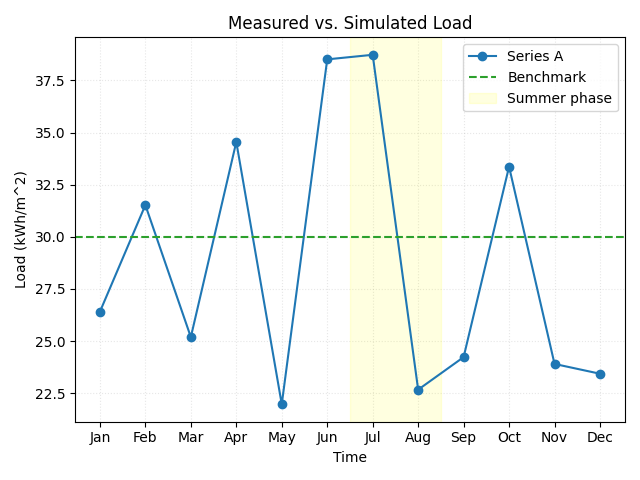
\includegraphics[width=0.6\linewidth]{Figures/Visualization/16.8.2.png}
    \caption{Axes helpers in practice: descriptive title and axis labels; categorical month ticks; a light dotted grid placed behind data for legibility; a dashed benchmark line at 30~kWh/m$^2$; and a shaded band highlighting the summer phase. These simple additions improve readability without clutter.}
    \label{fig:line_axes_helpers}
\end{figure}

\hhh{Comprehensive example: energy breakdown over a year}
Figure \ref{fig:energy_breakdown} shows the plot of this example.
\code{c16_detailed_line_plot}{python}{
    import matplotlib.pyplot as plt
    import numpy as np

    # Monthly data for a small office building
    months = ['Jan', 'Feb', 'Mar', 'Apr', 'May', 'Jun',
              'Jul', 'Aug', 'Sep', 'Oct', 'Nov', 'Dec']

    # Energy consumption data (kWh) - realistic values
    # Heating peaks in winter, cooling in summer
    heating = [4500, 3800, 3000, 1800, 800, 200,
               100, 100, 300, 1200, 2800, 4200]
    cooling = [200, 200, 400, 800, 1500, 2800,
               3500, 3400, 2200, 1000, 400, 200]

    # Base loads remain relatively constant
    lighting = [1200] * 12
    equipment = [1500] * 12

    # Total consumption
    total = [h + c + l + e for h, c, l, e in
             zip(heating, cooling, lighting, equipment)]

    # Figure and axes
    fig, ax = plt.subplots(figsize=(12, 7))

    # Lines with distinct styles and markers
    ax.plot(months, heating,   marker='o', linewidth=2.5,
            color='#E74C3C', label='Heating',   markersize=8)
    ax.plot(months, cooling,   marker='s', linewidth=2.5,
            color='#3498DB', label='Cooling',   markersize=8)
    ax.plot(months, lighting,  marker='^', linewidth=2.0,
            color='#F39C12', label='Lighting',  markersize=6, linestyle='--')
    ax.plot(months, equipment, marker='v', linewidth=2.0,
            color='#95A5A6', label='Equipment', markersize=6, linestyle='--')
    ax.plot(months, total,     marker='D', linewidth=3.0,
            color='#2C3E50', label='Total',     markersize=7, linestyle='-.')

    # Axes labeling and title
    ax.set_xlabel('Month', fontsize=12, fontweight='bold')
    ax.set_ylabel('Energy Consumption (kWh)', fontsize=12, fontweight='bold')
    ax.set_title('Monthly Energy Consumption Breakdown\nSmall Office Building (500 m$^2$)',
                 fontsize=14, fontweight='bold')

    # Grid behind data
    ax.grid(True, alpha=0.3, linestyle=':')
    ax.set_axisbelow(True)

    # Legend
    ax.legend(loc='upper left', frameon=True, shadow=True,
              title='Energy Type', title_fontsize=11)

    # Seasonal shading (indices: 0-based; spans are half-step padded)
    ax.axvspan(5.5, 7.5, alpha=0.1, color='yellow', label='Summer Peak')
    ax.axvspan(-0.5, 1.5, alpha=0.1, color='lightblue')
    ax.axvspan(10.5, 11.5, alpha=0.1, color='lightblue', label='Winter Peak')

    # Annotate peak total
    peak_month_idx = int(np.argmax(total))
    peak_value = total[peak_month_idx]
    ax.annotate(f'Peak: {peak_value:,.0f} kWh',
                xy=(peak_month_idx, peak_value),
                xytext=(peak_month_idx - 2, peak_value + 500),
                fontsize=10, fontweight='bold',
                arrowprops=dict(arrowstyle='->', color='red', lw=2),
                bbox=dict(boxstyle='round,pad=0.3',
                          facecolor='yellow', alpha=0.7))

    # Average line
    avg_total = float(np.mean(total))
    ax.axhline(y=avg_total, color='green', linestyle='--', linewidth=1, alpha=0.7)
    ax.text(11, avg_total + 100, f'Avg: {avg_total:,.0f} kWh',
            fontsize=10, color='green', fontweight='bold')

    # Label rotation (categorical months)
    plt.setp(ax.xaxis.get_majorticklabels(), rotation=0)

    # Optional: table of values (disabled in figure to avoid squeeze)
    # table_data = [[''] + months,
    #               ['Heating'] + [f'{h:,}' for h in heating],
    #               ['Cooling'] + [f'{c:,}' for c in cooling],
    #               ['Total'] +   [f'{t:,}' for t in total]]
    # ax.table(cellText=table_data, loc='bottom', cellLoc='center',
    #          bbox=[0, -0.3, 1, 0.2])

    plt.tight_layout()
    plt.show()

    # Console summary
    print("=" * 50)
    print("ENERGY ANALYSIS SUMMARY")
    print("=" * 50)
    print("Annual Consumption:")
    print(f"  Heating:   {sum(heating):,} kWh ({sum(heating)/sum(total)*100:.1f}%)")
    print(f"  Cooling:   {sum(cooling):,} kWh ({sum(cooling)/sum(total)*100:.1f}%)")
    print(f"  Lighting:  {sum(lighting):,} kWh ({sum(lighting)/sum(total)*100:.1f}%)")
    print(f"  Equipment: {sum(equipment):,} kWh ({sum(equipment)/sum(total)*100:.1f}%)")
    print(f"  TOTAL:     {sum(total):,} kWh")
    print(f"\nMonthly Average: {avg_total:,.0f} kWh")
    print(f"Peak Month: {months[peak_month_idx]} ({peak_value:,} kWh)")
    print(f"Energy Use Intensity: {sum(total)/500:.1f} kWh/m$^2$/year")

    # Outcome:
    # - Five lines with distinct styles and markers
    # - Seasonal shaded bands and benchmark line
    # - Peak annotation and labeled average
    # - Legend and grid for readability
}{Comprehensive line plot showing energy consumption patterns with detailed annotations}

\begin{figure}[bhtp]
    \centering
    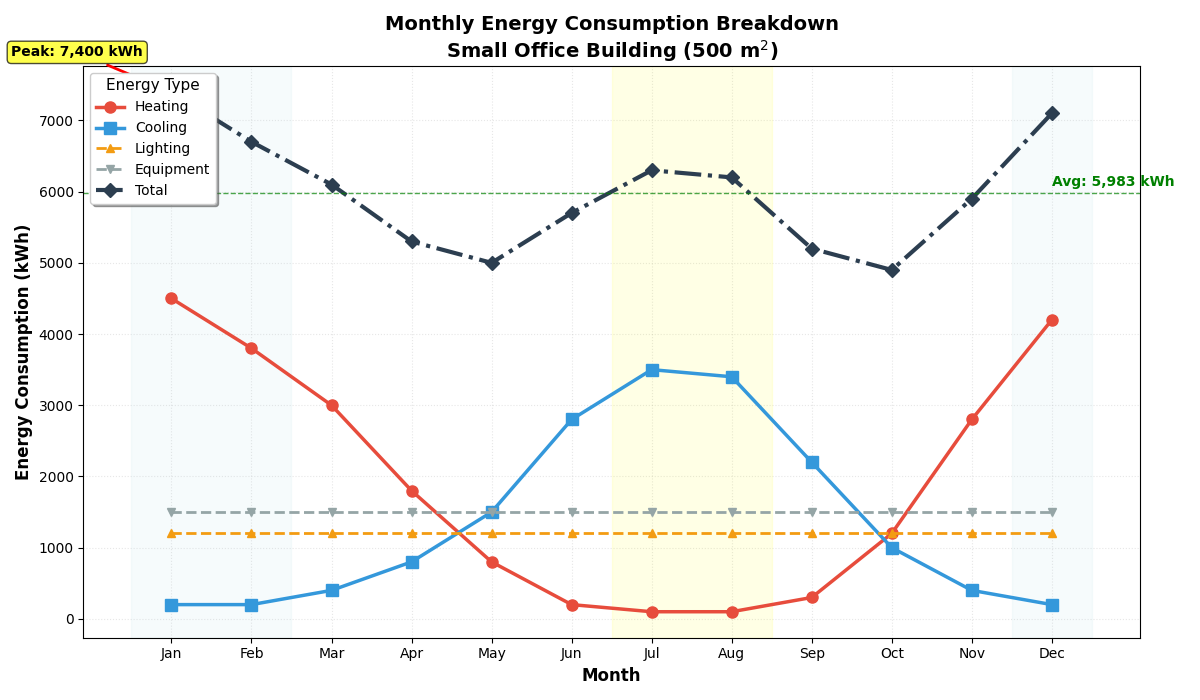
\includegraphics[width=0.65\linewidth]{Figures/Visualization/16.8.3.png}
    \caption{Energy breakdown over a year.}
    \label{fig:energy_breakdown}
\end{figure}

\hhh{Line plots (syntax quick reference)}

\textbf{Multiple lines with markers \& legend}\\  
When you compare two scenarios over the same x-axis, plot both lines with distinct markers/linestyles and include a legend. As shown in Figure~\ref{fig:line_multi}, markers make sampling explicit while linestyle differentiates the series at a glance.

\code{c16_line_multi}{python}{
    import numpy as np
    import matplotlib.pyplot as plt

    x = np.arange(12)
    y1 = np.sin(x/2) * 10 + 30
    y2 = np.cos(x/3) * 8 + 25

    fig, ax = plt.subplots()
    ax.plot(x, y1, marker='o', linewidth=2, label='Scenario A')
    ax.plot(x, y2, marker='s', linewidth=2, linestyle='--', label='Scenario B')

    ax.set_xlabel('Month index'); ax.set_ylabel('kWh/m$^2$')
    ax.legend(); ax.grid(True, linestyle=':', alpha=0.3)
    plt.tight_layout(); plt.show()
}{Two lines with styles and legend.}

\begin{figure}[htp!]
    \centering
    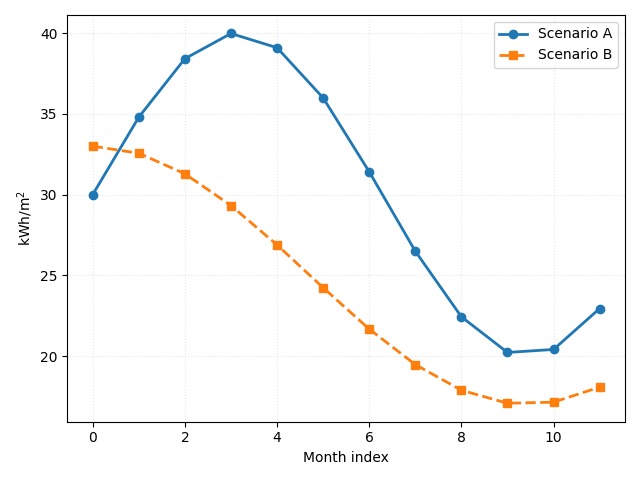
\includegraphics[width=0.5\linewidth]{Figures/Visualization/16.8.4.png}
    \caption{Comparing two scenarios with distinct markers and linestyles. The legend disambiguates the series, while a light dotted grid supports value reading without visual clutter.}
    \label{fig:line_multi}
\end{figure}

\medskip

\textbf{Datetime axis (proper spacing and tick formatting)}\\
Time series should use real dates on the x-axis so tick spacing/formatting respects calendar intervals. Figure~\ref{fig:line_datetime} illustrates weekly ticks (Mondays) and a compact month-day format that remains readable after \texttt{autofmt\_xdate()}.

\code{c16_line_datetime}{python}{
    import datetime as dt
    import numpy as np
    import matplotlib.pyplot as plt
    import matplotlib.dates as mdates

    dates = [dt.date(2025, 6, 1) + dt.timedelta(days=i) for i in range(30)]
    temps = 22 + 6*np.sin(np.arange(30)/5)

    fig, ax = plt.subplots(figsize=(9, 4))
    ax.plot(dates, temps, marker='o', markersize=3, linewidth=1.5, label='Temp')

    # Date ticks: weekly on Mondays, e.g., "Jun 02"
    ax.xaxis.set_major_locator(mdates.WeekdayLocator(byweekday=mdates.MO))
    ax.xaxis.set_major_formatter(mdates.DateFormatter('%b %d'))
    fig.autofmt_xdate()  # rotate/align dates

    ax.set_ylabel('deg C') 
    ax.legend(); ax.grid(True, linestyle=':', alpha=0.3)
    plt.tight_layout(); plt.show()
}{Datetime x-axis formatting.}

\begin{figure}[htp!]
    \centering
    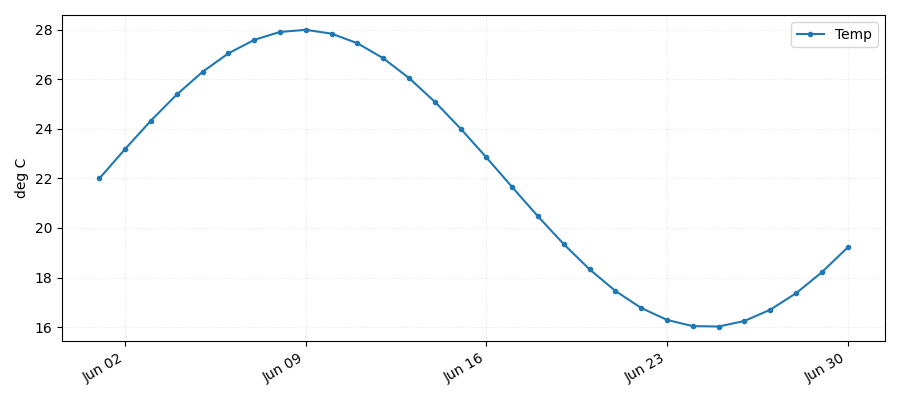
\includegraphics[width=0.5\linewidth]{Figures/Visualization/16.8.4b.png}
    \caption{Datetime axis with weekly ticks and a month–day formatter. Using date locators/formatters preserves true time spacing and prevents misleading “equal step” plots.}
    \label{fig:line_datetime}
\end{figure}

\medskip

\textbf{Fill area (bands for variation/uncertainty)}  \\
When you need to show tolerance, variation, or uncertainty around a line, add a translucent band using \texttt{fill\_between}. In Figure~\ref{fig:line_fill_between}, the shaded envelope conveys a \(\pm 2\ \text{kWh/m}^2\) range without obscuring the central trend.

\code{c16_line_fill_between}{python}{
    import numpy as np
    import matplotlib.pyplot as plt

    x = np.linspace(0, 10, 200)
    y = 20 + 5*np.sin(x)
    lo, hi = y - 2, y + 2  # band around the line

    fig, ax = plt.subplots()
    ax.plot(x, y, color='C0', label='Measured')
    ax.fill_between(x, lo, hi, color='C0', alpha=0.15, label='±2 kWh/m$^2$')

    ax.set_xlabel('Time (h)'); ax.set_ylabel('Load (kWh/m$^2$)')
    ax.legend(); ax.grid(True, linestyle=':', alpha=0.3)
    plt.tight_layout(); plt.show()
}{Shaded band around a line.}

\begin{figure}[htp!]
    \centering
    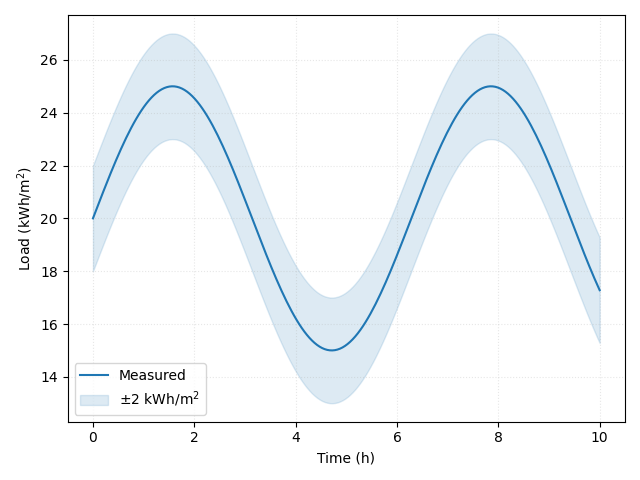
\includegraphics[width=0.5\linewidth]{Figures/Visualization/16.8.4c.png}
    \caption{Line with a translucent uncertainty band. The central series shows the measured load; the shaded envelope communicates expected variation without overwhelming the main signal.}
    \label{fig:line_fill_between}
\end{figure}

\medskip

\textbf{Twin axes (two units sharing x: energy \& temperature)}  \\
If two variables share the same x-axis but use different units, a twin y-axis can be acceptable—use sparingly and label clearly. Figure~\ref{fig:line_twin_axes} separates energy (left axis) and temperature (right axis) with color-matched labels and ticks to reduce confusion.

\code{c16_line_twin_axes}{python}{
    import numpy as np
    import matplotlib.pyplot as plt

    x = np.arange(12)
    kwh = np.linspace(1200, 1800, 12)         # energy
    temp = np.linspace(-5, 28, 12)            # temperature

    fig, ax1 = plt.subplots()
    ax1.plot(x, kwh, color='C3', marker='o', label='Energy (kWh)')
    ax1.set_ylabel('Energy (kWh)', color='C3'); ax1.tick_params(axis='y', colors='C3')

    ax2 = ax1.twinx()
    ax2.plot(x, temp, color='C0', linestyle='--', marker='s', label='Temp (deg C)')
    ax2.set_ylabel('Temperature (deg C)', color='C0'); ax2.tick_params(axis='y', colors='C0')

    ax1.set_xlabel('Month index'); ax1.grid(True, linestyle=':', alpha=0.3)
    fig.tight_layout(); plt.show()
}{Twin y-axes (use sparingly, label clearly).}

\begin{figure}[bhtp!]
    \centering
    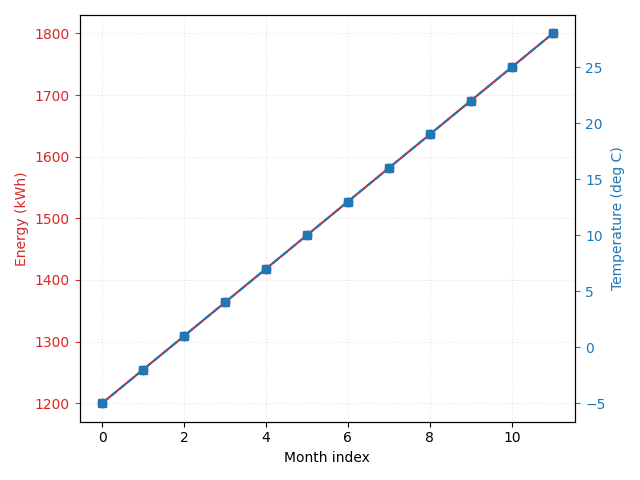
\includegraphics[width=0.5\linewidth]{Figures/Visualization/16.8.4d.png}
    \caption{Twin y-axes for variables with different units. Color-matching the curves and their y-axis labels reduces ambiguity; use this pattern only when dual scales improve comprehension.}
    \label{fig:line_twin_axes}
\end{figure}

\medskip

\textbf{Rolling average and missing data (gaps with NaN)}  \\
Real data often contain gaps. Plot NaNs as gaps to avoid misleading lines, then add a computed rolling mean for context. Figure~\ref{fig:line_nan_rolling} shows raw values (with breaks) alongside a simple 3-point mean that ignores NaNs.

\code{c16_line_nan_rolling}{python}{
    import numpy as np
    import matplotlib.pyplot as plt

    x = np.arange(20)
    y = np.array([10,12,11, np.nan, np.nan, 15,16,18,17,16,
                  14,15,14,13,12, 14,15, np.nan, 16,17])

    # Simple 3-point rolling mean ignoring NaN (demo)
    def rolling_mean(arr, k=3):
        out = np.full_like(arr, np.nan, dtype=float)
        for i in range(k-1, len(arr)):
            window = arr[i-k+1:i+1]
            vals = window[~np.isnan(window)]
            if len(vals) > 0:
                out[i] = vals.mean()
        return out

    y_smooth = rolling_mean(y, k=3)

    fig, ax = plt.subplots()
    ax.plot(x, y, marker='o', linewidth=1.2, label='Raw (with gaps)')
    ax.plot(x, y_smooth, color='C3', linewidth=2, label='3-pt mean')

    ax.set_xlabel('Index'); ax.set_ylabel('Value')
    ax.legend(); ax.grid(True, linestyle=':', alpha=0.3)
    plt.tight_layout(); plt.show()
}{Line gaps with NaN and a simple rolling mean.}

\begin{figure}[htp!]
    \centering
    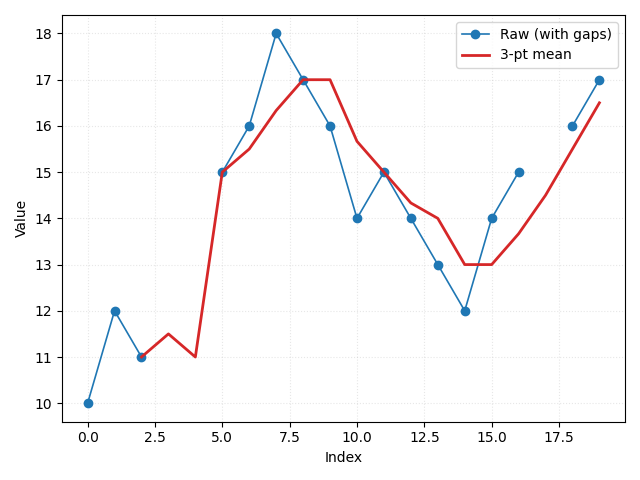
\includegraphics[width=0.5\linewidth]{Figures/Visualization/16.8.4e.png}
    \caption{Handling missing values in line plots. NaNs create visible gaps, preventing false continuity. A simple rolling mean provides context without pretending to know the missing observations.}
    \label{fig:line_nan_rolling}
\end{figure}


\textit{Notes}
\begin{itemize}
    \item Use the OO interface (\texttt{fig, ax = plt.subplots()}) for multi-axes layouts.
    \item For real calendars, prefer datetime or Pandas time indexes over categorical month strings.
    \item Bands (\texttt{fill\_between}) communicate variation/uncertainty better than a second thin line.
    \item Twin axes are helpful but can mislead if scales are chosen poorly—label clearly and consider color-coding ticks.
    \item Gaps (\texttt{NaN}) intentionally break lines; avoid interpolating unless justified.
\end{itemize}

\hh{Scatter plots: discovering relationships}

Scatter plots are essential for exploring relationships between two variables. In architectural practice, they reveal how design parameters affect performance (e.g., window area vs.\ daylight, insulation vs.\ heating demand). Each point represents one observation; patterns in the cloud indicate correlation or the lack thereof.

\textit{Figure~\ref{fig:scatter_simple}} introduces the idea with a minimal example—synthetic data with a gentle positive trend. After that, \textit{Figure~\ref{fig:scatter_detailed}} presents a richer, architectural use case: daylight performance across rooms, with encodings for color, size, target bands, and trend lines.

\medskip

\textbf{Simple scatter example}  \\
A compact demo to show axes, points, and an optional best-fit trend line (nothing else).

\code{c16_scatter_simple}{python}{
    import matplotlib.pyplot as plt
    import numpy as np

    # Simple synthetic relationship: y grows with x plus noise
    rng = np.random.default_rng(0)
    x = np.linspace(0, 10, 40)
    y = 2.0 * x + rng.normal(0, 4, size=x.size)

    fig, ax = plt.subplots(figsize=(6, 4))
    ax.scatter(x, y, s=40, alpha=0.8, edgecolors='black', linewidth=0.6)

    # Optional: simple least-squares fit
    m, b = np.polyfit(x, y, 1)
    ax.plot(x, m * x + b, linestyle='--', linewidth=1.5, label=f'Fit: y={m:.2f}x+{b:.2f}')

    ax.set_xlabel('X (input)')
    ax.set_ylabel('Y (response)')
    ax.set_title('Simple scatter with optional trend line')
    ax.grid(True, linestyle=':', alpha=0.3)
    ax.legend()
    plt.tight_layout(); plt.show()
}{A minimal scatter plot with an optional best-fit line.}

\begin{figure}[bhtp!]
    \centering
    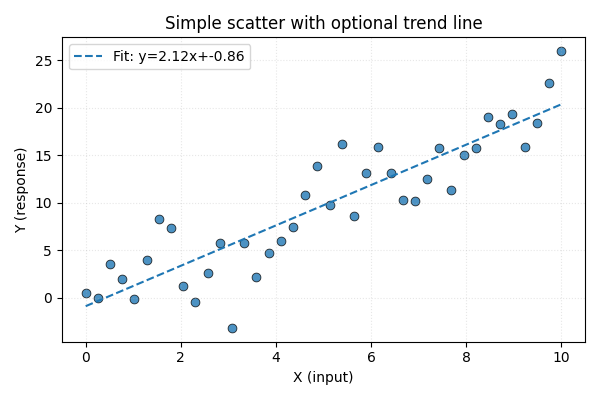
\includegraphics[width=0.6\linewidth]{Figures/Visualization/16.9.png}
    \caption{Introductory scatter plot. Each point shows a single observation; the dashed line is an optional least-squares fit. Use this pattern when first assessing whether a relationship might exist (direction, strength, and outliers).}
    \label{fig:scatter_simple}
\end{figure}

\medskip

\textbf{Comprehensive scatter (architectural daylight analysis)} \\ 
In Figure~\ref{fig:scatter_detailed}, two coordinated scatter plots explore how geometry influences daylight: left—Window-to-Floor Ratio (WFR) vs.\ Daylight Factor (DF) with a polynomial trend and target bands; right—Depth vs.\ DF with a rule-of-thumb guide. Color maps and point sizes encode additional variables (depth, window/floor area), supporting multi-criteria design decisions.

\code{c16_scatter_detailed}{python}{
    import matplotlib.pyplot as plt
    import numpy as np
    
    # Daylight analysis for 40 rooms in an office building
    # We'll explore how room geometry affects daylight
    
    # Set random seed for reproducibility
    np.random.seed(42)
    
    # Generate realistic room data
    n_rooms = 40
    
    # Room dimensions
    room_depths = np.random.uniform(4, 10, n_rooms)  # meters from window
    window_areas = np.random.uniform(3, 20, n_rooms)  # m2 of glazing
    floor_areas = np.random.uniform(20, 60, n_rooms)  # m2 floor area
    
    # Calculate Window-to-Floor Ratio (WFR)
    wfr = (window_areas / floor_areas) * 100  # as percentage
    
    # Daylight Factor calculation (simplified model)
    # DF increases with window area, decreases with room depth
    # Add some random variation to simulate real measurements
    daylight_factor = (window_areas / (room_depths * floor_areas**0.5)) * 15
    daylight_factor *= np.random.uniform(0.8, 1.2, n_rooms)  # Add variation
    
    # Create figure with 2 subplots side by side
    fig, (ax1, ax2) = plt.subplots(1, 2, figsize=(14, 6))
    
    # SUBPLOT 1: Window-to-Floor Ratio vs Daylight Factor
    scatter1 = ax1.scatter(wfr, daylight_factor, 
                          c=room_depths,  # Color by room depth
                          cmap='viridis_r',  # Color map (reversed)
                          s=100,  # Point size
                          alpha=0.7,  # Transparency
                          edgecolors='black',  # Black borders
                          linewidth=1)
    
    # Add target zones (building code requirements)
    ax1.axhspan(2, 5, alpha=0.15, color='green', label='Target DF (2-5%)')
    ax1.axvspan(15, 25, alpha=0.15, color='blue', label='Target WFR (15-25%)')
    
    # Add trend line using polynomial fit
    z = np.polyfit(wfr, daylight_factor, 2)  # 2nd degree polynomial
    p = np.poly1d(z)
    x_trend = np.linspace(min(wfr), max(wfr), 100)
    ax1.plot(x_trend, p(x_trend), 'r--', alpha=0.5, 
             linewidth=2, label='Trend')
    
    # Labels and formatting for subplot 1
    ax1.set_xlabel('Window-to-Floor Ratio (%)', fontsize=11, fontweight='bold')
    ax1.set_ylabel('Daylight Factor (%)', fontsize=11, fontweight='bold')
    ax1.set_title('Daylight vs Window-to-Floor Ratio', fontsize=12, fontweight='bold')
    ax1.grid(True, alpha=0.3, linestyle=':')
    ax1.legend(loc='upper left', fontsize=10)
    
    # Add colorbar for room depth
    cbar1 = plt.colorbar(scatter1, ax=ax1)
    cbar1.set_label('Room Depth (m)', rotation=270, labelpad=20, fontsize=10)
    
    # SUBPLOT 2: Room Depth vs Daylight Factor
    # Size points by window area this time
    scatter2 = ax2.scatter(room_depths, daylight_factor,
                          c=window_areas,  # Color by window area
                          cmap='coolwarm',
                          s=floor_areas * 3,  # Size by floor area
                          alpha=0.7,
                          edgecolors='black',
                          linewidth=1)
    
    # Add target daylight zone
    ax2.axhspan(2, 5, alpha=0.15, color='green', label='Target DF (2-5%)')
    
    # Add rule of thumb line (DF = 10/depth)
    depth_range = np.linspace(4, 10, 50)
    rule_of_thumb = 10 / depth_range
    ax2.plot(depth_range, rule_of_thumb, 'b--', alpha=0.5,
             linewidth=2, label='Rule of thumb')
    
    # Labels and formatting for subplot 2
    ax2.set_xlabel('Room Depth (m)', fontsize=11, fontweight='bold')
    ax2.set_ylabel('Daylight Factor (%)', fontsize=11, fontweight='bold')
    ax2.set_title('Daylight vs Room Depth', fontsize=12, fontweight='bold')
    ax2.grid(True, alpha=0.3, linestyle=':')
    ax2.legend(loc='upper right', fontsize=10)
    
    # Add colorbar for window area
    cbar2 = plt.colorbar(scatter2, ax=ax2)
    cbar2.set_label('Window Area (m2)', rotation=270, labelpad=20, fontsize=10)
    
    # Overall title
    fig.suptitle('DAYLIGHT ANALYSIS: 40 Office Rooms', 
                 fontsize=14, fontweight='bold')
    
    plt.tight_layout()
    plt.show()
    
    # Analysis and recommendations
    print("=" * 60)
    print("DAYLIGHT ANALYSIS RESULTS")
    print("=" * 60)
    
    # Identify well-daylit rooms (DF between 2-5%)
    good_daylight = (daylight_factor >= 2) & (daylight_factor <= 5)
    n_good = good_daylight.sum()
    
    print(f"Rooms meeting daylight target (2-5% DF): {n_good}/{n_rooms} ({n_good/n_rooms*100:.1f}%)")
    
    # Statistics for good rooms
    if n_good > 0:
        avg_depth_good = room_depths[good_daylight].mean()
        avg_wfr_good = wfr[good_daylight].mean()
        avg_window_good = window_areas[good_daylight].mean()
        
        print(f"\nCharacteristics of well-daylit rooms:")
        print(f"  Average room depth: {avg_depth_good:.1f} m")
        print(f"  Average WFR: {avg_wfr_good:.1f}%")
        print(f"  Average window area: {avg_window_good:.1f} m2")
    
    # Identify problem rooms
    poor_daylight = daylight_factor < 2
    n_poor = poor_daylight.sum()
    
    if n_poor > 0:
        print(f"\nRooms with poor daylight (<2% DF): {n_poor}")
        avg_depth_poor = room_depths[poor_daylight].mean()
        avg_window_poor = window_areas[poor_daylight].mean()
        print(f"  Average room depth: {avg_depth_poor:.1f} m")
        print(f"  Average window area: {avg_window_poor:.1f} m2")
        print(f"  Recommendation: Increase glazing or reduce room depth")
    
    # Correlation analysis
    from scipy.stats import pearsonr
    corr_wfr, _ = pearsonr(wfr, daylight_factor)
    corr_depth, _ = pearsonr(room_depths, daylight_factor)
    
    print(f"\nCorrelation Analysis:")
    print(f"  WFR vs DF correlation: {corr_wfr:.3f} (strong positive)")
    print(f"  Depth vs DF correlation: {corr_depth:.3f} (negative)")

}{Comprehensive scatter plot analysis exploring daylight performance factors.}

\begin{figure}[htp!]
    \centering
    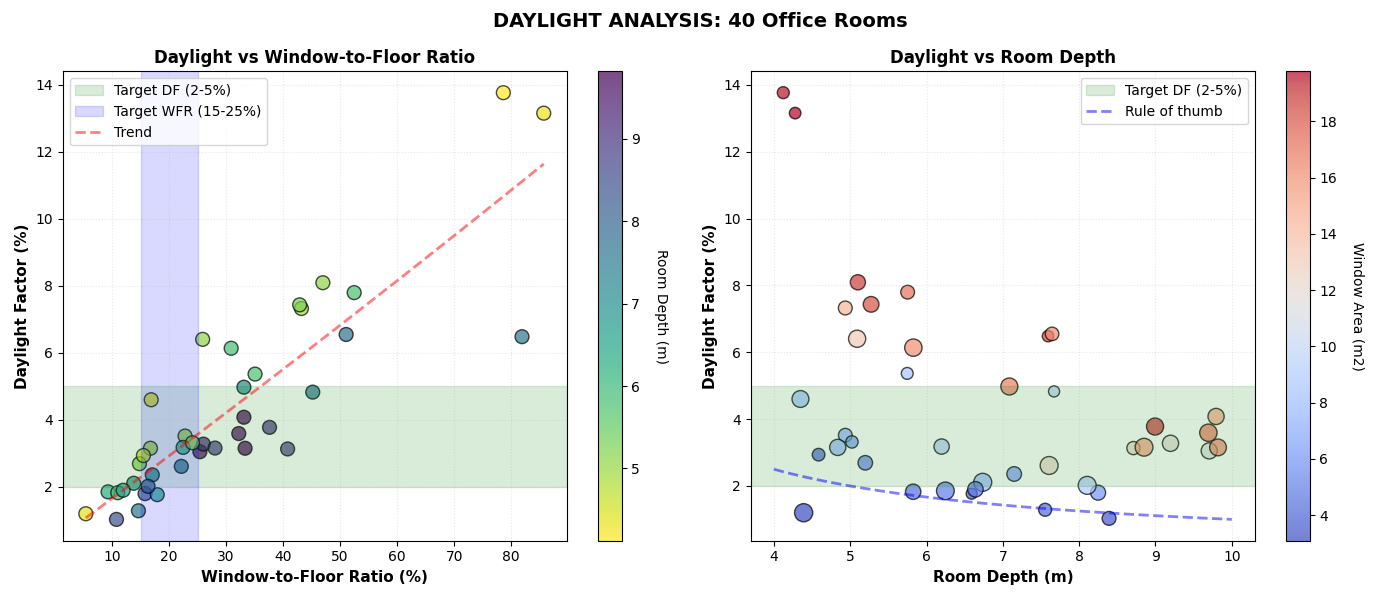
\includegraphics[width=1\linewidth]{Figures/Visualization/16.9b.png}
    \caption{Two coordinated scatter plots for daylight analysis. Left: Window-to-Floor Ratio (WFR) vs.\ Daylight Factor (DF), with depth-coded color, target bands, and a fitted trend. Right: Room depth vs.\ DF, with window-area color, floor-area size, and a rule-of-thumb guide. Together, these views reveal how geometry influences daylight and where adjustments might improve performance.}
    \label{fig:scatter_detailed}
\end{figure}

\hh{Heat maps: visualizing data across two dimensions}
\textbf{Core syntax — arguments and parameters}. Heat maps display how a value varies across two independent dimensions by mapping values to color. In architecture they are ideal for facade temperature or solar gain by orientation and month, occupancy by room and hour, or space utilization across floors and days. Think of a heat map as a colorized table where color encodes magnitude—hot spots, cold zones, and gradients become immediately visible.

\textit{Figure~\ref{fig:hm_imshow}} illustrates the core \texttt{imshow} pattern for a regular grid; \textit{Figure~\ref{fig:hm_pcolor}} shows \texttt{pcolormesh} on a nonuniform grid; and \textit{Figure~\ref{fig:hm_contourf}} presents \texttt{contourf} when you want smooth bands/regions. \textit{Figure~\ref{fig:hm_norms}} compares colorbar/normalization options, while \textit{Figure~\ref{fig:hm_labels}} and \textit{Figure~\ref{fig:hm_helpers}} demonstrate labeling and per-cell annotations.

\hhh{imshow (fast for dense, regularly spaced grids)}  
As shown in Figure~\ref{fig:hm_imshow}, \texttt{imshow} maps a 2D array \texttt{Z} directly to pixel cells.

\code{c16_heatmap_imshow_syntax}{python}{
    import numpy as np
    import matplotlib.pyplot as plt

    # Example data: 8 orientations x 12 months (solar-like pattern)
    rng = np.random.default_rng(0)
    base = np.linspace(0, 1, 12)[None, :]
    orient = np.linspace(0.6, 1.0, 8)[:, None]
    Z = 100 * orient * (0.5 + 0.5 * np.sin(2*np.pi*(base - 0.25))) + rng.normal(0, 5, (8, 12))

    fig, ax = plt.subplots(figsize=(7.2, 4.2))
    im = ax.imshow(Z, cmap='YlOrRd', vmin=0, vmax=100, aspect='auto', origin='upper')
    ax.set_title('Heat map via imshow')
    ax.set_xlabel('Month'); ax.set_ylabel('Orientation index')

    cbar = plt.colorbar(im, ax=ax, fraction=0.046, pad=0.04)
    cbar.set_label('Solar gain (kWh/m$^2$)', rotation=270, labelpad=16)

    plt.tight_layout(); plt.show()
}{\texttt{imshow} for regular grids: \texttt{cmap}, \texttt{vmin}/\texttt{vmax}, \texttt{aspect}, \texttt{origin}.}

\begin{figure}[htp!]
    \centering
    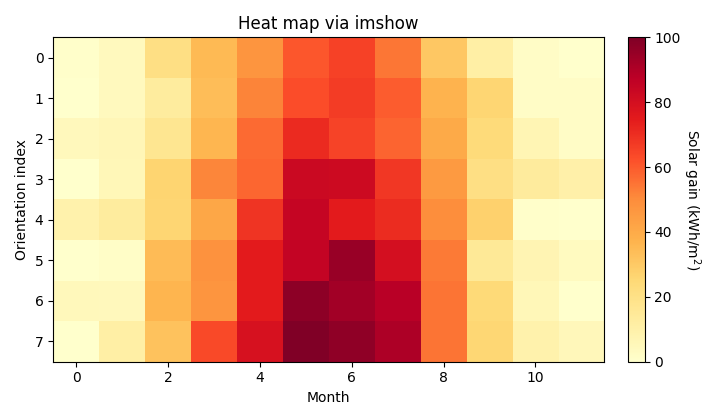
\includegraphics[width=0.6\linewidth]{Figures/Visualization/16.10.1.png}
    \caption{Regular-grid heat map using \texttt{imshow}. The 2D array is rendered as pixel cells; a labeled colorbar conveys the value scale.}
    \label{fig:hm_imshow}
\end{figure}

\medskip

\hhh{pcolormesh (flexible for nonuniform or masked grids)}  
Figure~\ref{fig:hm_pcolor} demonstrates \texttt{pcolormesh} with nonuniform bin edges and a masked region.

\code{c16_heatmap_pcolormesh_syntax}{python}{
    import numpy as np
    import matplotlib.pyplot as plt

    # Nonuniform axes (e.g., irregular months or custom coordinates)
    x_edges = np.array([0, 1, 1.8, 3.2, 5.5, 6.0, 8.0, 10.5])
    y_edges = np.array([0, 2, 3, 4.5, 6.5, 9.0])

    # Cell-centered values Z must be (len(y_edges)-1, len(x_edges)-1)
    rng = np.random.default_rng(1)
    Z = rng.uniform(0, 1, size=(len(y_edges)-1, len(x_edges)-1))
    Z[2, 3] = np.nan  # masked cell example

    fig, ax = plt.subplots(figsize=(7.2, 4.2))
    qm = ax.pcolormesh(x_edges, y_edges, Z, cmap='plasma', shading='auto')
    ax.set_title('Heat map via pcolormesh (nonuniform bins)')
    ax.set_xlabel('X (nonuniform)'); ax.set_ylabel('Y (nonuniform)')

    cbar = plt.colorbar(qm, ax=ax, fraction=0.046, pad=0.04)
    cbar.set_label('Value (unit)', rotation=270, labelpad=16)

    plt.tight_layout(); plt.show()
}{\texttt{pcolormesh} for nonuniform/edge-defined grids; NaNs appear masked.}

\begin{figure}[htp!]
    \centering
    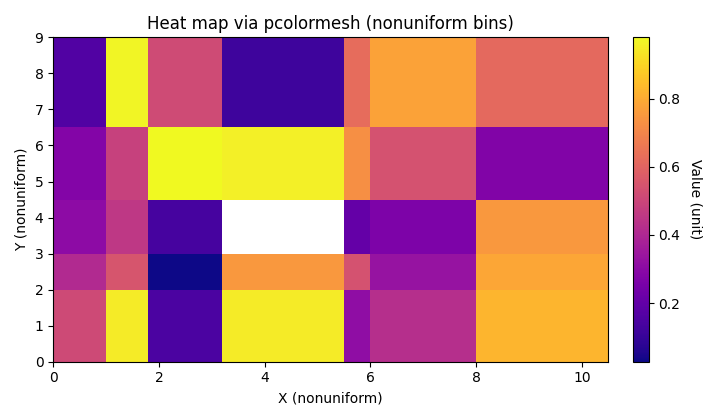
\includegraphics[width=0.6\linewidth]{Figures/Visualization/16.10.2}
    \caption{\texttt{pcolormesh} on a nonuniform grid. Bin edges define the cell geometry; NaN values create masked (empty) cells.}
    \label{fig:hm_pcolor}
\end{figure}

\medskip

\hhh{contourf (filled contours for smoothed region bands)}  
As in Figure~\ref{fig:hm_contourf}, \texttt{contourf} groups values into smooth bands and can overlay isolines.

\code{c16_heatmap_contourf_syntax}{python}{
    import numpy as np
    import matplotlib.pyplot as plt

    x = np.linspace(-3, 3, 120)
    y = np.linspace(-2, 2, 90)
    X, Y = np.meshgrid(x, y, indexing='xy')
    Z = 2*np.exp(-(X**2 + (Y*1.5)**2)) + 0.4*np.cos(2*X) - 0.3*np.sin(2*Y)

    fig, ax = plt.subplots(figsize=(7.2, 4.2))
    cf = ax.contourf(X, Y, Z, levels=14, cmap='viridis')
    lines = ax.contour(X, Y, Z, levels=10, colors='white', linewidths=0.8, alpha=0.6)
    ax.clabel(lines, inline=True, fontsize=8)

    ax.set_title('Filled contours via contourf')
    ax.set_xlabel('X'); ax.set_ylabel('Y')

    cbar = plt.colorbar(cf, ax=ax, fraction=0.046, pad=0.04)
    cbar.set_label('Value', rotation=270, labelpad=16)

    plt.tight_layout(); plt.show()
}{contourf for smooth bands; optional isolines with contour.}

\begin{figure}[htp!]
    \centering
    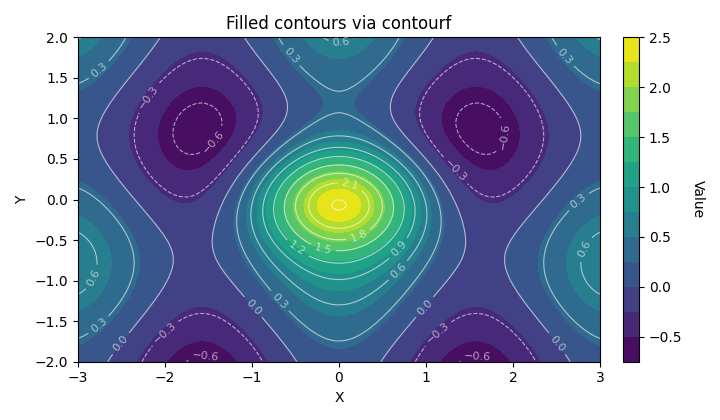
\includegraphics[width=0.6\linewidth]{Figures/Visualization/16.10.3.png}
    \caption{Filled-contour heat map. Smooth bands reveal gradients; white isolines add quantitative landmarks.}
    \label{fig:hm_contourf}
\end{figure}

\medskip

\hhh{Colorbars, colormaps, and normalization}
Figure~\ref{fig:hm_norms} compares linear mapping, diverging mapping centered on a reference, and logarithmic mapping.

\code{c16_heatmap_colorbar_norm}{python}{
    import numpy as np
    import matplotlib.pyplot as plt
    import matplotlib.colors as mcolors

    rng = np.random.default_rng(2)
    Z_lin = rng.uniform(0, 100, size=(20, 30))
    Z_div = rng.normal(0, 1, size=(20, 30)) * 50
    Z_log = rng.uniform(1, 1e3, size=(20, 30))

    fig, axes = plt.subplots(1, 3, figsize=(12, 3.8))

    im0 = axes[0].imshow(Z_lin, cmap='YlOrRd', vmin=0, vmax=100, aspect='auto')
    axes[0].set_title('Linear (Normalize)')
    plt.colorbar(im0, ax=axes[0], fraction=0.046, pad=0.04).set_label('Units')

    norm_div = mcolors.TwoSlopeNorm(vmin=-150, vcenter=0, vmax=150)
    im1 = axes[1].imshow(Z_div, cmap='coolwarm', norm=norm_div, aspect='auto')
    axes[1].set_title('Diverging (TwoSlopeNorm)')
    plt.colorbar(im1, ax=axes[1], fraction=0.046, pad=0.04).set_label('Deviation')

    im2 = axes[2].imshow(Z_log, cmap='plasma', norm=mcolors.LogNorm(), aspect='auto')
    axes[2].set_title('Log (LogNorm)')
    plt.colorbar(im2, ax=axes[2], fraction=0.046, pad=0.04).set_label('Magnitude')

    for ax in axes: ax.set_axis_off()
    plt.tight_layout(); plt.show()
}{Colorbar + normalization patterns: linear, diverging, logarithmic.}

\begin{figure}[htp!]
    \centering
    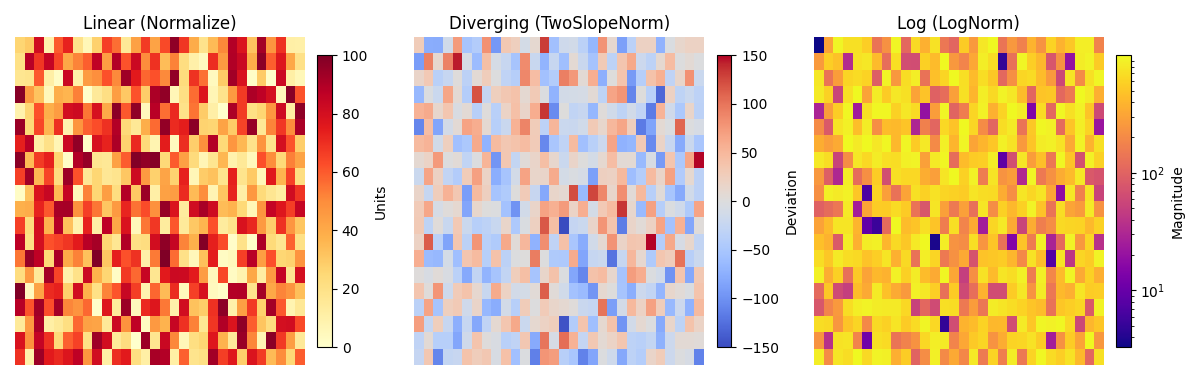
\includegraphics[width=1\linewidth]{Figures/Visualization/16.10.4.png}
    \caption{Normalization comparison. Left: linear mapping 0–100. Middle: diverging map centered at 0 to emphasize over/under performance. Right: logarithmic mapping for wide dynamic ranges.}
    \label{fig:hm_norms}
\end{figure}

\medskip

\hhh{Indexing and labels}
In Figure~\ref{fig:hm_labels}, we assign category tick labels to rows/columns and rotate the x-labels for readability.

\code{c16_heatmap_labels}{python}{
    import numpy as np
    import matplotlib.pyplot as plt

    # Example: 6 rooms x 8 months with synthetic usage index
    rng = np.random.default_rng(3)
    Z = np.clip(60 + 25*np.sin(np.linspace(0, 2*np.pi, 8))[None, :] + rng.normal(0, 8, (6, 8)), 0, 100)

    row_labels = [f'Room {i+1}' for i in range(Z.shape[0])]
    col_labels = ['Jan','Feb','Mar','Apr','May','Jun','Jul','Aug']

    fig, ax = plt.subplots(figsize=(8, 4.6))
    im = ax.imshow(Z, cmap='viridis', vmin=0, vmax=100, aspect='auto')

    ax.set_xticks(np.arange(Z.shape[1])); ax.set_yticks(np.arange(Z.shape[0]))
    ax.set_xticklabels(col_labels, rotation=45, ha='right')
    ax.set_yticklabels(row_labels)
    ax.set_xlabel('Month'); ax.set_ylabel('Room')

    cbar = plt.colorbar(im, ax=ax, fraction=0.046, pad=0.04)
    cbar.set_label('Usage index (%)', rotation=270, labelpad=16)

    plt.tight_layout(); plt.show()
}{Ticks and category labels on rows/columns.}

\begin{figure}[htp!]
    \centering
    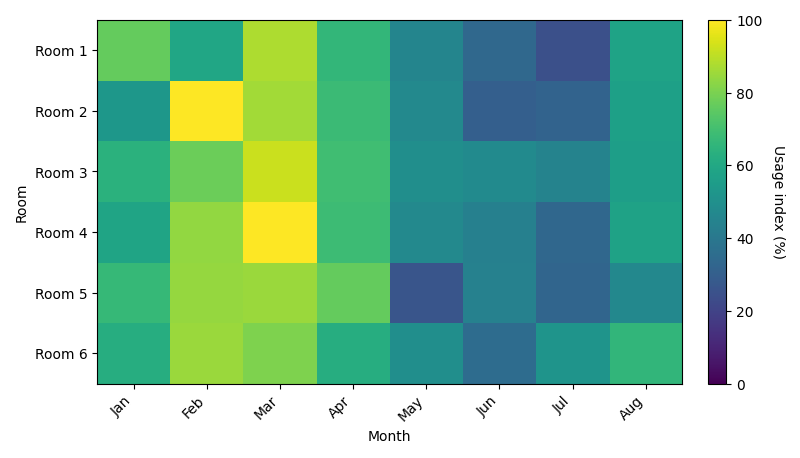
\includegraphics[width=0.6\linewidth]{Figures/Visualization/16.10.5.png}
    \caption{Labeled heat map with categorical ticks. Rotated x-labels prevent overlap; a colorbar with units clarifies meaning.}
    \label{fig:hm_labels}
\end{figure}

\hhh{Axes helpers for heat maps (annotations, grid, layout)}

Figure~\ref{fig:hm_helpers} adds per-cell annotations and a labeled colorbar. Use annotation sparingly—great for compact matrices, overwhelming on large grids.

\code{c16_heatmap_axes_helpers}{python}{
    import numpy as np
    import matplotlib.pyplot as plt

    # Small matrix where per-cell labels are useful
    Z = np.array([
        [18, 22, 35, 45],
        [28, 36, 40, 52],
        [12, 20, 26, 31]
    ], dtype=float)

    fig, ax = plt.subplots(figsize=(6.4, 3.8))

    im = ax.imshow(Z, cmap='YlOrRd', aspect='auto')

    # Annotate each cell
    for i in range(Z.shape[0]):
        for j in range(Z.shape[1]):
            val = Z[i, j]
            ax.text(j, i, f'{val:.0f}',
                    ha='center', va='center',
                    color=('white' if val > Z.max()*0.6 else 'black'),
                    fontsize=9)

    # Colorbar with label
    cbar = plt.colorbar(im, ax=ax, fraction=0.046, pad=0.04)
    cbar.set_label('Value (units)', rotation=270, labelpad=16)

    ax.set_title('Per-cell labels with colorbar', pad=8)
    ax.set_xlabel('Column'); ax.set_ylabel('Row')
    ax.set_axisbelow(True)
    ax.grid(False)
    plt.tight_layout(); plt.show()
}{Adding per-cell labels and a colorbar.}

\begin{figure}[htp!]
    \centering
    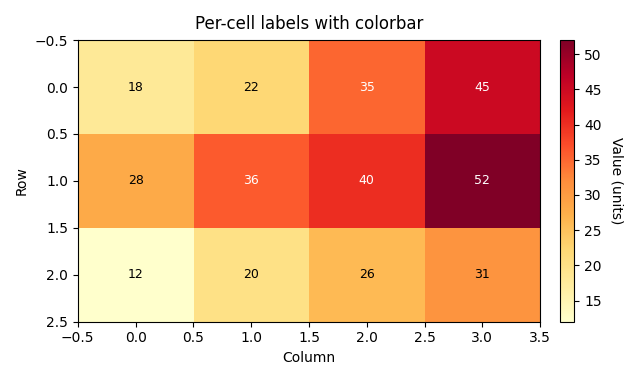
\includegraphics[width=0.6\linewidth]{Figures/Visualization/16.10.6.png}
    \caption{Per-cell annotation on a small grid. Text shows cell values while color communicates magnitude; best used for compact matrices.}
    \label{fig:hm_helpers}
\end{figure}

\hhh{Detailed example: facade solar by orientation and month}

Figure~\ref{fig:heatmap_detailed} presents two complementary views of the same dataset: (left) a regular-grid heat map with per-cell value labels for exact readings, and (right) a smoothed \texttt{contourf} view with isolines that emphasize gradients and peak zones. Together, these views make seasonal and orientation effects immediately legible.

\code{c16_heatmap_detailed}{python}{
    import numpy as np
    import matplotlib.pyplot as plt
    from scipy.interpolate import RegularGridInterpolator

    orientations = ['N','NE','E','SE','S','SW','W','NW']
    months = ['Jan','Feb','Mar','Apr','May','Jun','Jul','Aug','Sep','Oct','Nov','Dec']

    Z = np.array([
        [20, 22, 35, 45, 55, 60, 58, 48, 38, 28, 22, 18],  # N
        [25, 30, 45, 58, 70, 75, 73, 62, 48, 35, 28, 23],  # NE
        [35, 42, 60, 75, 85, 90, 88, 78, 65, 48, 38, 32],  # E
        [45, 55, 75, 88, 95, 98, 96, 90, 78, 62, 48, 42],  # SE
        [50, 60, 80, 92, 98, 100, 99, 94, 82, 68, 52, 46], # S
        [45, 55, 75, 88, 95, 98, 96, 90, 78, 62, 48, 42],  # SW
        [35, 42, 60, 75, 85, 90, 88, 78, 65, 48, 38, 32],  # W
        [25, 30, 45, 58, 70, 75, 73, 62, 48, 35, 28, 23],  # NW
    ])

    fig, (ax1, ax2) = plt.subplots(1, 2, figsize=(16, 6))

    # ----------------------------------------------------------
    # Heat map 1: values
    # ----------------------------------------------------------
    im1 = ax1.imshow(Z, cmap='YlOrRd', aspect='auto')
    ax1.set_xticks(np.arange(len(months)));  ax1.set_xticklabels(months, rotation=45, ha="right")
    ax1.set_yticks(np.arange(len(orientations)));  ax1.set_yticklabels(orientations)
    cbar1 = plt.colorbar(im1, ax=ax1);  cbar1.set_label('Solar (kWh/m$^2$/month)', rotation=270, labelpad=20)

    for i in range(len(orientations)):
        for j in range(len(months)):
            val = Z[i, j]
            ax1.text(j, i, f'{val:.0f}', ha="center", va="center",
                     color=('white' if val > 60 else 'black'), fontsize=8)

    ax1.set_title('Solar by Orientation and Month (With Values)', fontsize=12, fontweight='bold')
    ax1.set_xlabel('Month'); ax1.set_ylabel('Facade Orientation')

    # ----------------------------------------------------------
    # Heat map 2: smooth contours via RegularGridInterpolator
    # ----------------------------------------------------------
    x = np.arange(len(months))       # 0..11 (columns)
    y = np.arange(len(orientations)) # 0..7  (rows)
    rgi = RegularGridInterpolator((y, x), Z, method="linear",
                                  bounds_error=False, fill_value=np.nan)

    xi = np.linspace(0, len(x)-1, 100)
    yi = np.linspace(0, len(y)-1, 100)
    Xi, Yi = np.meshgrid(xi, yi, indexing="xy")
    Zsmooth = rgi(np.stack([Yi.ravel(), Xi.ravel()], axis=-1)).reshape(Yi.shape)

    im2 = ax2.contourf(Xi, Yi, Zsmooth, levels=15, cmap='plasma')
    lines = ax2.contour(Xi, Yi, Zsmooth, levels=8, colors='white', alpha=0.4, linewidths=1)
    ax2.clabel(lines, inline=True, fontsize=8, fmt='%d')

    ax2.set_xticks(np.linspace(0, len(x)-1, len(months))); ax2.set_xticklabels(months, rotation=45, ha="right")
    ax2.set_yticks(np.linspace(0, len(y)-1, len(orientations))); ax2.set_yticklabels(orientations)
    cbar2 = plt.colorbar(im2, ax=ax2); cbar2.set_label('Solar (kWh/m$^2$/month)', rotation=270, labelpad=20)

    # Mark top radiation zones (>= 95% of max) in the same coord system
    max_val = Z.max()
    I, J = np.where(Z >= 0.95 * max_val)
    for i, j in zip(I, J):
        ax2.scatter(j, i, marker='*', s=200, color='yellow',
                    edgecolor='black', linewidth=1, zorder=10)

    ax2.set_xlim(0, len(x)-1); ax2.set_ylim(0, len(y)-1)
    ax2.set_title('Solar by Orientation and Month (Smooth Contours)', fontsize=12, fontweight='bold')
    ax2.set_xlabel('Month'); ax2.set_ylabel('Facade Orientation')

    plt.suptitle('FACADE SOLAR ANALYSIS', fontsize=14, fontweight='bold')
    plt.tight_layout()
    plt.show()

    # ----------------------------------------------------------
    # Analysis outcomes (printed to console)
    # ----------------------------------------------------------
    print("=" * 60)
    print("SOLAR RADIATION ANALYSIS")
    print("=" * 60)

    # Annual totals by orientation
    annual_totals = Z.sum(axis=1)  # sum over months
    print("\nAnnual Solar Radiation by Orientation:")
    for orient, total in zip(orientations, annual_totals):
        print(f"  {orient:3s}: {total:.0f} kWh/m$^2$/year")

    # Best / minimal orientations
    best_orient = orientations[int(annual_totals.argmax())]
    min_orient  = orientations[int(annual_totals.argmin())]
    print(f"\nBest orientation for solar panels: {best_orient}")
    print(f"Best orientation for minimal heat gain: {min_orient}")

    # Seasonal patterns
    winter_idx = [0, 1, 11]  # Jan, Feb, Dec
    summer_idx = [5, 6, 7]   # Jun, Jul, Aug
    winter_avg = Z[:, winter_idx].mean(axis=1)
    summer_avg = Z[:, summer_idx].mean(axis=1)

    print("\nSeasonal Patterns:")
    print(f"  Highest summer radiation: {orientations[int(summer_avg.argmax())]} ({summer_avg.max():.1f} kWh/m$^2$/month avg)")
    print(f"  Lowest winter  radiation: {orientations[int(winter_avg.argmin())]} ({winter_avg.min():.1f} kWh/m$^2$/month avg)")

    # Simple design recommendations
    print("\nDESIGN RECOMMENDATIONS:")
    print("  - Favor S/SE/SW for passive solar collection where overheating can be managed.")
    print("  - Provide shading on S/SE/SW facades during summer months.")
    print("  - North-facing facades are suitable for consistent daylighting with lower heat gain.")
    print("  - Consider additional shading for E/W facades due to low-angle morning/evening sun.")
}{Creating heat maps for two-dimensional building performance data.}

\begin{figure}[htp!]
    \centering
    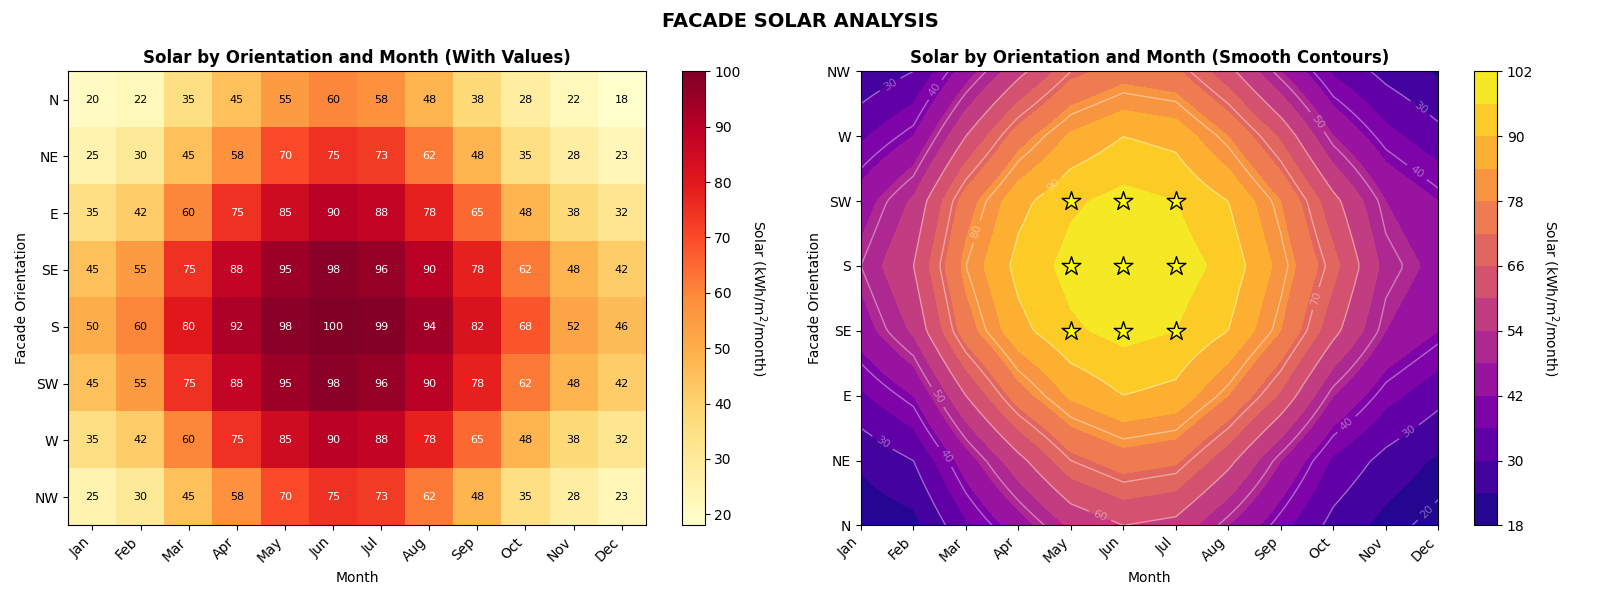
\includegraphics[width=\linewidth]{Figures/Visualization/16.10.7.png}
    \caption{Facade solar by orientation and month: two coordinated views. Left—regular-grid heat map with per-cell values; right—smoothed contours with isolines and star markers at $\geq 95\%$ of the maximum. The pair reveals absolute values and gradients for seasonal/orientation decisions.}
    \label{fig:heatmap_detailed}
\end{figure}

\hhh{Heat maps (syntax quick reference)}

\textbf{1) Annotated grid with \texttt{imshow}}\\  
Use \texttt{imshow} for dense regular grids and add per-cell text only for small matrices to avoid clutter (see Figure~\ref{fig:hm_quick_annot}).

\code{c16_heatmap_quick_annot}{python}{
    import numpy as np
    import matplotlib.pyplot as plt

    Z = np.random.randint(10, 100, size=(6, 8))
    fig, ax = plt.subplots(figsize=(8, 4))
    im = ax.imshow(Z, cmap='viridis', aspect='auto', vmin=0, vmax=100)

    # Axis labels
    ax.set_xticks(np.arange(8)); ax.set_yticks(np.arange(6))
    ax.set_xticklabels([f'C{j+1}' for j in range(8)], rotation=45, ha='right')
    ax.set_yticklabels([f'R{i+1}' for i in range(6)])

    # Per-cell text
    for i in range(Z.shape[0]):
        for j in range(Z.shape[1]):
            ax.text(j, i, f'{Z[i, j]}', ha='center', va='center', fontsize=8)

    plt.colorbar(im, ax=ax).set_label('Units')
    plt.tight_layout(); plt.show()
}{Values printed inside each cell.}

\begin{figure}[htp!]
    \centering
    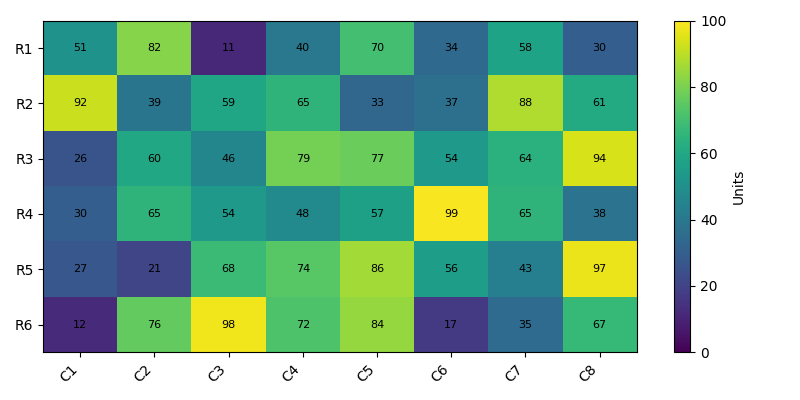
\includegraphics[width=0.6\linewidth]{Figures/Visualization/16.10.8.1.png}
    \caption{Annotated \texttt{imshow} grid (small matrix). Exact values appear as text; a colorbar communicates the scale.}
    \label{fig:hm_quick_annot}
\end{figure}

\medskip

\textbf{2) Masked NaN data with \texttt{pcolormesh}}\\  
When data are missing or irregular, \texttt{pcolormesh} respects NaNs and nonuniform bins (Figure~\ref{fig:hm_quick_mask}).

\code{c16_heatmap_quick_mask}{python}{
    import numpy as np
    import matplotlib.pyplot as plt
    Z = np.random.rand(20, 30)
    Z[5:8, 10:15] = np.nan  # missing block

    fig, ax = plt.subplots()
    pcm = ax.pcolormesh(Z, cmap='magma', shading='auto')
    plt.colorbar(pcm, ax=ax).set_label('Value')

    ax.set_title('Masked region (NaN) in heat map')
    plt.tight_layout(); plt.show()
}{Masked data (holes) rendered as blanks.}

\begin{figure}[htp!]
    \centering
    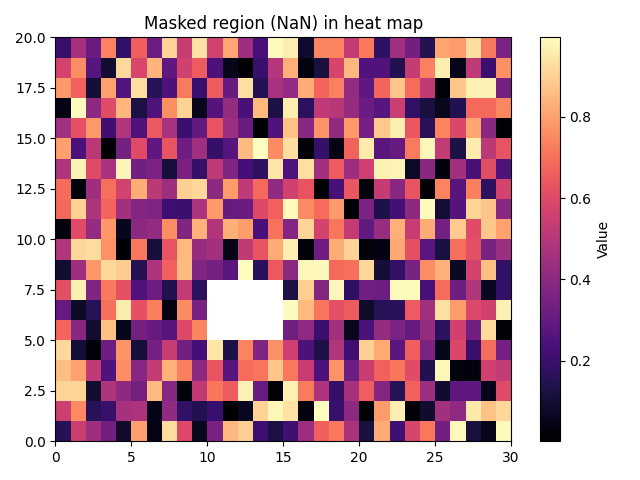
\includegraphics[width=0.6\linewidth]{Figures/Visualization/16.10.8.2.png}
    \caption{\texttt{pcolormesh} with NaNs. Missing blocks render as empty cells; use when bin edges are irregular or parts of the grid are undefined.}
    \label{fig:hm_quick_mask}
\end{figure}

\medskip

\textbf{3) Diverging map centered at zero}\\  
For deviations around a meaningful reference (e.g., target = 0), use a diverging colormap with \texttt{TwoSlopeNorm} (Figure~\ref{fig:hm_quick_diverging}).

\code{c16_heatmap_quick_diverging}{python}{
    import numpy as np
    import matplotlib.pyplot as plt
    import matplotlib.colors as mcolors

    Z = np.random.randn(50, 50) * 5  # negative and positive deviations
    norm = mcolors.TwoSlopeNorm(vmin=-15, vcenter=0, vmax=15)

    fig, ax = plt.subplots()
    im = ax.imshow(Z, cmap='coolwarm', norm=norm)
    plt.colorbar(im, ax=ax).set_label('Deviation (units)')
    ax.set_title('Diverging heat map centered at zero')
    plt.tight_layout(); plt.show()
}{Center color at a reference value.}

\begin{figure}[htp!]
    \centering
    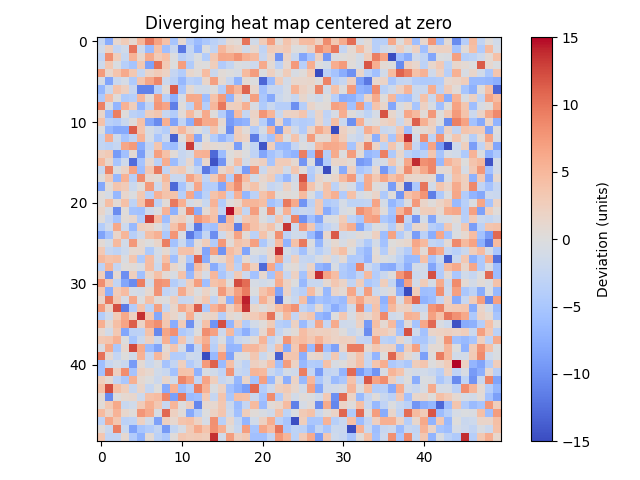
\includegraphics[width=0.6\linewidth]{Figures/Visualization/16.10.8.3.png}
    \caption{Diverging heat map around a reference (0). Warm and cool hues emphasize over- vs.\ under-performance relative to the center.}
    \label{fig:hm_quick_diverging}
\end{figure}

\medskip

\textbf{4) Discrete bins with labeled colorbar}\\  
When communicating categories or thresholds, bin continuous data and use a \texttt{BoundaryNorm} so the legend matches the bins (Figure~\ref{fig:hm_quick_bins}).

\code{c16_heatmap_quick_bins}{python}{
    import numpy as np
    import matplotlib.pyplot as plt
    import matplotlib.colors as mcolors

    Z = np.random.rand(30, 30) * 100
    bins = [0, 20, 40, 60, 80, 100]
    cmap = plt.get_cmap('YlOrRd', len(bins)-1)
    norm = mcolors.BoundaryNorm(bins, cmap.N)

    fig, ax = plt.subplots()
    im = ax.imshow(Z, cmap=cmap, norm=norm)
    cbar = plt.colorbar(im, ax=ax, ticks=bins)
    cbar.set_label('Score (%)')
    ax.set_title('Binned heat map with discrete legend')
    plt.tight_layout(); plt.show()
}{Discrete classes and matching legend.}

\begin{figure}[htp!]
    \centering
    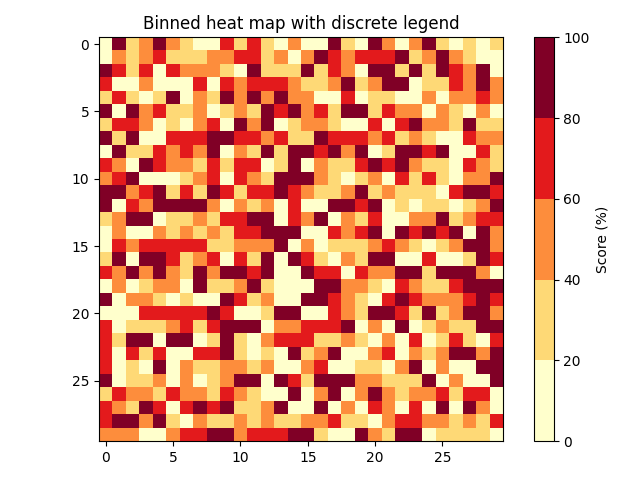
\includegraphics[width=0.6\linewidth]{Figures/Visualization/16.10.8.4.png}
    \caption{Discrete, binned heat map. Class breaks (0–20–40–60–80–100) are encoded with a stepped colormap and a matching ticked colorbar.}
    \label{fig:hm_quick_bins}
\end{figure}


\hhh{Common pitfalls and checklist}

\begin{itemize}
    \item \textbf{Label both axes clearly.} Heat maps are 2D tables; unlabeled rows/columns make them unreadable.
    \item \textbf{Choose an appropriate colormap.} Sequential (e.g., \texttt{YlOrRd}) for magnitude, diverging (e.g., \texttt{coolwarm}) when values cross a meaningful center (e.g., 0).
    \item \textbf{Fix the value range.} Set \texttt{vmin/vmax} (or a \texttt{Norm}) so colors are comparable across subplots/figures.
    \item \textbf{Use \texttt{origin} and \texttt{extent} thoughtfully.} Make sure the visual orientation matches the conceptual one (north at top? month order left to right?).
    \item \textbf{Avoid heavy gridlines.} They fight with the pixel grid; per-cell annotations or subtle ticks usually read better.
    \item \textbf{Beware interpolation.} Smooth interpolation can imply nonexistent data; state when you are smoothing and why.
\end{itemize}

\hhh{Comprehensive example: Building multi-panel dashboards}

Real architectural analysis rarely fits in a single plot—you need dashboards that combine multiple views to tell a coherent story. Think of dashboards as presentation boards for data: multiple, related panels arranged to answer complementary questions. Start with the overview, then drill into detail; keep colors and scales consistent across comparable metrics; and use whitespace, titles, and annotations to guide the reader.

Figure~\ref{fig:building_dashboard} illustrates this approach with a six-panel layout: (1) a stacked area chart summarizing space allocation by floor, (2) energy use per floor with a twin-axis occupancy overlay, (3) a pie chart of total space distribution, (4) box plots comparing energy variation by use type, (5) a weekly \(\,7\times24\,\) occupancy heat map, and (6) a summary panel of key metrics. Together, the panels move from high-level composition to performance details and actionable takeaways.

\code{c16_dashboard_detailed}{python}{
    import matplotlib.pyplot as plt
    import numpy as np
    from matplotlib.gridspec import GridSpec
    
    # Comprehensive building performance dashboard
    # Analyzing a 10-floor mixed-use building
    
    # Generate realistic building data
    np.random.seed(42)
    
    floors = np.arange(1, 11)  # 10 floors
    floor_names = [f'Floor {i}' for i in floors]
    
    # Space allocation by floor (m2)
    office_area = np.array([0, 0, 450, 480, 490, 485, 475, 470, 460, 450])
    retail_area = np.array([580, 550, 50, 20, 10, 10, 10, 10, 20, 30])
    residential_area = np.array([0, 0, 100, 120, 140, 145, 155, 160, 150, 140])
    circulation_area = np.array([120, 150, 100, 80, 60, 60, 60, 60, 70, 80])
    
    total_area = office_area + retail_area + residential_area + circulation_area
    
    # Energy consumption by floor (kWh/month)
    energy_base = np.array([850, 820, 650, 600, 580, 570, 560, 550, 540, 530])
    energy_variation = np.random.normal(0, 50, 10)
    energy_consumption = energy_base + energy_variation
    
    # Occupancy data (people)
    max_occupancy = np.array([150, 140, 85, 75, 70, 68, 65, 63, 60, 58])
    typical_occupancy = max_occupancy * np.random.uniform(0.7, 0.9, 10)
    
    # Create figure with custom layout using GridSpec
    fig = plt.figure(figsize=(16, 12))
    gs = GridSpec(3, 3, figure=fig, hspace=0.3, wspace=0.3)
    
    # Title for entire dashboard
    fig.suptitle('MIXED-USE BUILDING PERFORMANCE DASHBOARD\\n10 Floors | 7,000 m2 Total',
                 fontsize=16, fontweight='bold', y=0.98)
    
    # PANEL 1: Stacked area chart (space allocation)
    ax1 = fig.add_subplot(gs[0, :])  # Top row, all columns
    
    # Create stacked area chart
    ax1.fill_between(floors, 0, retail_area, 
                     color='#FF6B6B', label='Retail', alpha=0.8)
    ax1.fill_between(floors, retail_area, retail_area + office_area,
                     color='#4ECDC4', label='Office', alpha=0.8)
    ax1.fill_between(floors, retail_area + office_area, 
                     retail_area + office_area + residential_area,
                     color='#45B7D1', label='Residential', alpha=0.8)
    ax1.fill_between(floors, retail_area + office_area + residential_area,
                     total_area, color='#95A5A6', label='Circulation', alpha=0.8)
    
    ax1.set_xlabel('Floor', fontsize=11)
    ax1.set_ylabel('Area (m2)', fontsize=11)
    ax1.set_title('Space Allocation by Floor', fontsize=12, fontweight='bold')
    ax1.legend(loc='upper right', ncol=4, frameon=True, shadow=True)
    ax1.grid(True, alpha=0.3, linestyle=':')
    ax1.set_xlim(1, 10)
    
    # Add transition annotations
    ax1.annotate('Retail to Office\\nTransition', xy=(2.5, 400),
                xytext=(1, 550), fontsize=9,
                arrowprops=dict(arrowstyle='->', color='red', lw=1.5),
                bbox=dict(boxstyle='round', facecolor='wheat', alpha=0.8))
    
    # PANEL 2: Bar chart with line overlay (energy vs occupancy)
    ax2 = fig.add_subplot(gs[1, 0])  # Middle row, left column
    
    # Bar chart for energy
    bars = ax2.bar(floors, energy_consumption, color='#E74C3C', 
                   alpha=0.7, label='Energy Use')
    
    # Overlay line for occupancy (using secondary y-axis)
    ax2_twin = ax2.twinx()
    line = ax2_twin.plot(floors, typical_occupancy, 'o-', 
                        color='#3498DB', linewidth=2.5, 
                        markersize=8, label='Occupancy')
    
    ax2.set_xlabel('Floor', fontsize=11)
    ax2.set_ylabel('Energy (kWh/month)', fontsize=11, color='#E74C3C')
    ax2_twin.set_ylabel('Occupancy (people)', fontsize=11, color='#3498DB')
    ax2.set_title('Energy vs Occupancy', fontsize=12, fontweight='bold')
    ax2.grid(True, alpha=0.3, linestyle=':')
    
    # Color y-axis labels to match data
    ax2.tick_params(axis='y', labelcolor='#E74C3C')
    ax2_twin.tick_params(axis='y', labelcolor='#3498DB')
    
    # PANEL 3: Pie chart (total space distribution)
    ax3 = fig.add_subplot(gs[1, 1])  # Middle row, middle column
    
    total_office = office_area.sum()
    total_retail = retail_area.sum()
    total_residential = residential_area.sum()
    total_circulation = circulation_area.sum()
    
    sizes = [total_retail, total_office, total_residential, total_circulation]
    labels = ['Retail\\n' + f'{total_retail:.0f} m2',
              'Office\\n' + f'{total_office:.0f} m2',
              'Residential\\n' + f'{total_residential:.0f} m2',
              'Circulation\\n' + f'{total_circulation:.0f} m2']
    colors = ['#FF6B6B', '#4ECDC4', '#45B7D1', '#95A5A6']
    explode = (0.05, 0.05, 0.05, 0.05)  # Slightly separate all slices
    
    wedges, texts, autotexts = ax3.pie(sizes, labels=labels, colors=colors,
                                        explode=explode, autopct='%1.1f%%',
                                        shadow=True, startangle=45)
    
    # Improve text appearance
    for text in texts:
        text.set_fontsize(10)
    for autotext in autotexts:
        autotext.set_color('white')
        autotext.set_fontsize(10)
        autotext.set_fontweight('bold')
    
    ax3.set_title('Total Space Distribution', fontsize=12, fontweight='bold')
    
    # PANEL 4: Box plot (energy variation by use type)
    ax4 = fig.add_subplot(gs[1, 2])  # Middle row, right column
    
    # Generate energy consumption data by space type
    retail_floors = [1, 2]
    office_floors = [3, 4, 5, 6, 7, 8, 9, 10]
    mixed_floors = [3, 4, 5, 6, 7, 8]  # Floors with residential
    
    retail_energy = energy_consumption[0:2]
    office_energy = energy_consumption[2:10]
    mixed_energy = energy_consumption[2:8]
    
    # Add some variation for visualization
    retail_samples = np.random.normal(retail_energy.mean(), 30, 20)
    office_samples = np.random.normal(office_energy.mean(), 25, 30)
    mixed_samples = np.random.normal(mixed_energy.mean(), 20, 25)
    
    box_data = [retail_samples, office_samples, mixed_samples]
    box_labels = ['Retail\\nFloors', 'Office\\nFloors', 'Mixed\\nFloors']
    
    bp = ax4.boxplot(box_data, labels=box_labels, patch_artist=True)
    
    # Color the boxes
    box_colors = ['#FF6B6B', '#4ECDC4', '#9B59B6']
    for patch, color in zip(bp['boxes'], box_colors):
        patch.set_facecolor(color)
        patch.set_alpha(0.7)
    
    ax4.set_ylabel('Energy (kWh/month)', fontsize=11)
    ax4.set_title('Energy Distribution by Use Type', fontsize=12, fontweight='bold')
    ax4.grid(True, alpha=0.3, linestyle=':', axis='y')
    
    # PANEL 5: Heat map (hourly occupancy pattern)
    ax5 = fig.add_subplot(gs[2, :2])  # Bottom row, first two columns
    
    # Generate hourly occupancy pattern
    days = ['Mon', 'Tue', 'Wed', 'Thu', 'Fri', 'Sat', 'Sun']
    hours = [f'{h:02d}:00' for h in range(24)]
    
    # Create occupancy pattern (percentage of max)
    occupancy_pattern = np.zeros((7, 24))
    
    # Weekday patterns (Mon-Fri)
    for d in range(5):
        # Low at night
        occupancy_pattern[d, 0:7] = np.random.uniform(5, 10, 7)
        # Morning rise
        occupancy_pattern[d, 7:9] = np.random.uniform(40, 60, 2)
        # Workday high
        occupancy_pattern[d, 9:17] = np.random.uniform(70, 90, 8)
        # Evening decline
        occupancy_pattern[d, 17:21] = np.random.uniform(30, 50, 4)
        # Night low
        occupancy_pattern[d, 21:24] = np.random.uniform(10, 20, 3)
    
    # Weekend patterns
    for d in range(5, 7):
        occupancy_pattern[d, :] = np.random.uniform(20, 40, 24)
        # Retail peak on weekend afternoons
        occupancy_pattern[d, 12:18] = np.random.uniform(60, 80, 6)
    
    im = ax5.imshow(occupancy_pattern, cmap='RdYlGn_r', aspect='auto', vmin=0, vmax=100)
    
    # Set ticks
    ax5.set_xticks(np.arange(0, 24, 2))
    ax5.set_xticklabels(hours[::2], fontsize=9)
    ax5.set_yticks(np.arange(7))
    ax5.set_yticklabels(days)
    
    ax5.set_xlabel('Hour of Day', fontsize=11)
    ax5.set_ylabel('Day of Week', fontsize=11)
    ax5.set_title('Building Occupancy Pattern (% of Maximum)', 
                  fontsize=12, fontweight='bold')
    
    # Add colorbar
    cbar = plt.colorbar(im, ax=ax5)
    cbar.set_label('Occupancy %', rotation=270, labelpad=15)
    
    # PANEL 6: Summary statistics table
    ax6 = fig.add_subplot(gs[2, 2])  # Bottom row, right column
    ax6.axis('off')  # Turn off axes for text display
    
    # Calculate summary statistics
    total_building_area = total_area.sum()
    avg_energy = energy_consumption.mean()
    energy_intensity = avg_energy / (total_building_area / 10)  # per floor
    peak_occupancy = max_occupancy.sum()
    
    # Create summary text
    summary_text = "BUILDING SUMMARY\\n" + "=" * 25 + "\\n\\n"
    summary_text += f"Total Area: {total_building_area:,.0f} m2\\n"
    summary_text += f"Floors: {len(floors)}\\n"
    summary_text += f"Avg Floor Area: {total_building_area/10:.0f} m2\\n\\n"
    
    summary_text += "SPACE BREAKDOWN\\n" + "-" * 25 + "\\n"
    summary_text += f"Office: {total_office:,.0f} m2 ({total_office/total_building_area*100:.1f}%)\\n"
    summary_text += f"Retail: {total_retail:,.0f} m2 ({total_retail/total_building_area*100:.1f}%)\\n"
    summary_text += f"Residential: {total_residential:,.0f} m2 ({total_residential/total_building_area*100:.1f}%)\\n"
    summary_text += f"Circulation: {total_circulation:,.0f} m2 ({total_circulation/total_building_area*100:.1f}%)\\n\\n"
    
    summary_text += "PERFORMANCE\\n" + "-" * 25 + "\\n"
    summary_text += f"Avg Energy: {avg_energy:.0f} kWh/month\\n"
    summary_text += f"Energy Intensity: {energy_intensity:.1f} kWh/m2\\n"
    summary_text += f"Peak Occupancy: {peak_occupancy:.0f} people\\n"
    summary_text += f"Density: {total_building_area/peak_occupancy:.1f} m2/person"
    
    ax6.text(0.1, 0.9, summary_text, transform=ax6.transAxes,
            fontsize=10, verticalalignment='top',
            fontfamily='monospace',
            bbox=dict(boxstyle='round', facecolor='lightgray', alpha=0.8))
    
    plt.tight_layout()
    plt.show()
    
    # Print additional analysis
    print("=" * 60)
    print("DETAILED BUILDING ANALYSIS")
    print("=" * 60)
    print(f"\\nBuilding Type: Mixed-Use")
    print(f"Configuration:")
    print(f"  Floors 1-2: Primarily Retail ({retail_area[0:2].mean():.0f} m2/floor avg)")
    print(f"  Floors 3-10: Office + Residential Mix")
    print(f"\\nEfficiency Metrics:")
    print(f"  Net-to-Gross Ratio: {(total_building_area-total_circulation)/total_building_area*100:.1f}%")
    print(f"  Retail Loading: {peak_occupancy/total_retail:.2f} people/m2")
    print(f"  Office Loading: {peak_occupancy/total_office:.3f} people/m2")
    
    # Outcome:
    # A comprehensive 6-panel dashboard showing:
    #
    # Panel 1 (top): Stacked area chart
    # - Shows transition from retail (red) at bottom to office (cyan) above
    # - Circulation (gray) consistent across floors
    # - Annotation highlighting the transition zone
    #
    # Panel 2 (middle-left): Bar chart with line overlay
    # - Red bars show energy consumption decreasing with height
    # - Blue line shows occupancy following similar pattern
    # - Dual y-axes for different units
    #
    # Panel 3 (middle-center): Pie chart
    # - Visual breakdown of total space by type
    # - Percentages and areas shown
    # - Office dominates at ~45% of total
    #
    # Panel 4 (middle-right): Box plots
    # - Shows energy variation by floor type
    # - Retail floors have highest consumption
    # - Mixed floors show moderate variation
    #
    # Panel 5 (bottom-left): Heat map
    # - 7x24 grid showing weekly occupancy patterns
    # - Weekdays show clear 9-5 pattern (green/yellow)
    # - Weekends show retail afternoon peaks
    #
    # Panel 6 (bottom-right): Summary statistics
    # - Key metrics in monospace font
    # - Gray box with all essential numbers
    # - Space breakdown, performance metrics
}{Creating a comprehensive multi-panel dashboard for building analysis.}

\begin{figure}[htp!]
    \centering
    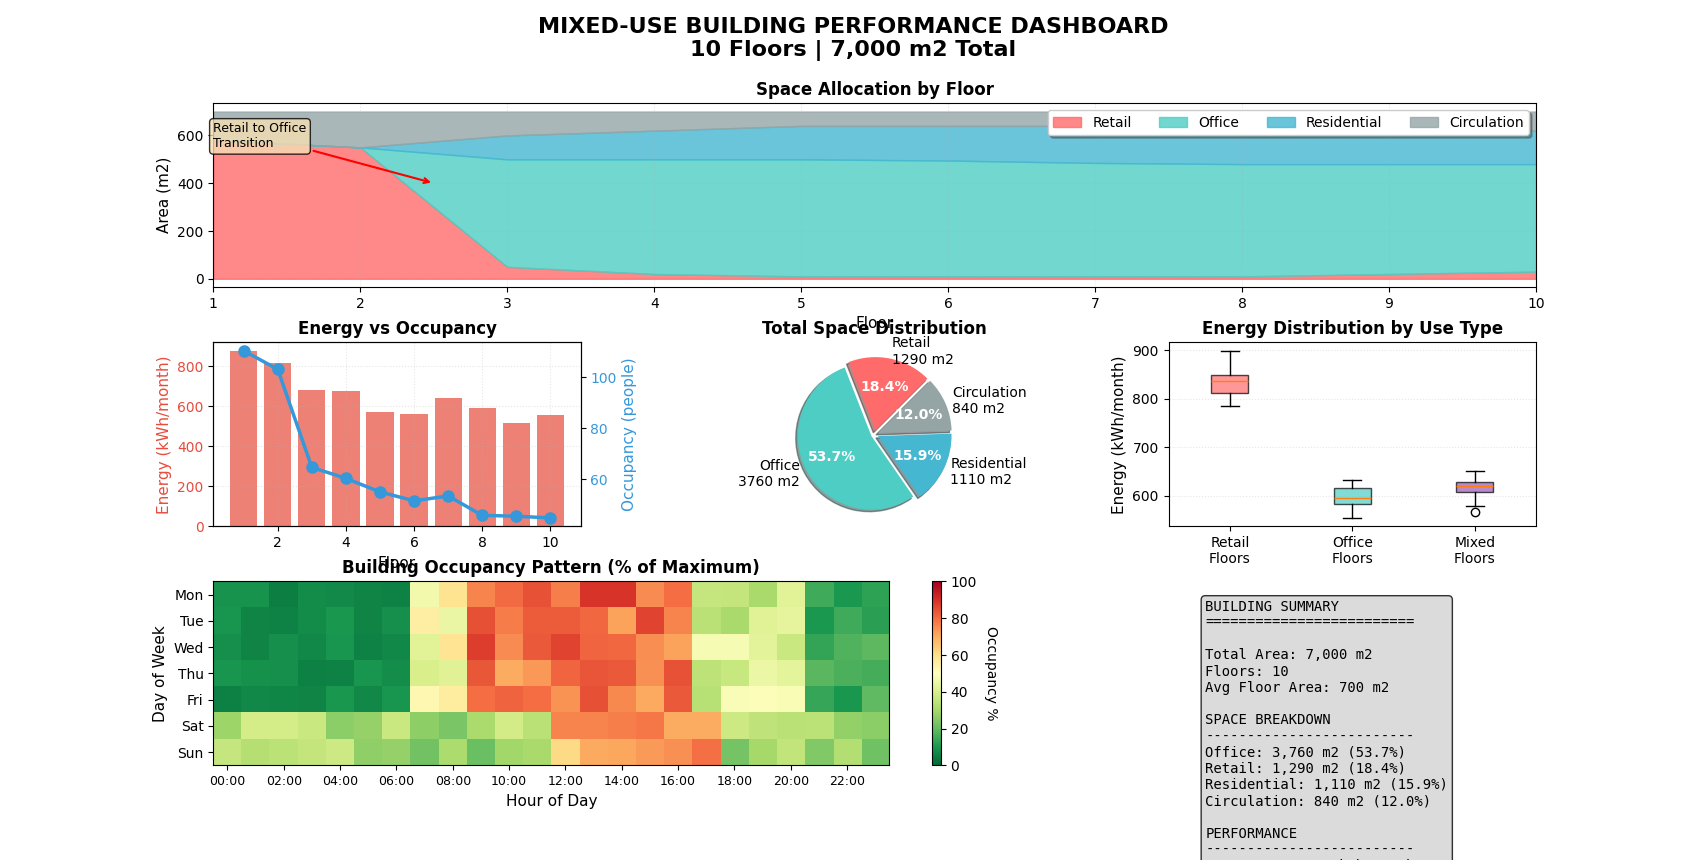
\includegraphics[width=1.05\linewidth]{Figures/Visualization/16.10.10.png}
    \caption{Multi-panel building performance dashboard. Top: stacked area chart summarizes space allocation by floor and highlights the retail-to-office transition. Middle row: energy vs.\ occupancy with twin axes (left), total space distribution (center), and energy variation by floor type via box plots (right). Bottom row: weekly \(7\times24\) occupancy heat map (left) and a text panel with key summary metrics (right).}
    \label{fig:building_dashboard}
\end{figure}

\hh{Customizing plot appearance }

Figure~\ref{fig:customization_v3} compares two side-by-side plots: a default bar chart and a customized version with architectural palette, better spacing, and annotations. This updated version fixes title overlap, moves legends outside, and uses real line breaks in tick labels.

\code{c16_customization_detailed_v3}{python}{
    import matplotlib.pyplot as plt
    import numpy as np

    categories = ['Site Area', 'Building\nFootprint', 'Green\nSpace',
                  'Parking', 'Total\nFloor Area', 'Efficiency']
    design_a = np.array([100, 40, 35, 25, 160, 75])
    design_b = np.array([100, 35, 45, 20, 175, 82])
    x = np.arange(len(categories))
    width = 0.35

    fig, (ax1, ax2) = plt.subplots(1, 2, figsize=(16, 7))

    # --- Left subplot: default-style comparison ---
    ax1.bar(x - width/2, design_a, width, label='Design A')
    ax1.bar(x + width/2, design_b, width, label='Design B')
    ax1.set_title('Building Design Comparison — DEFAULT', fontsize=12, pad=6)
    ax1.set_xlabel('Metrics')
    ax1.set_ylabel('Value')
    ax1.set_xticks(x)
    ax1.set_xticklabels(categories)
    ax1.legend(loc='upper left')
    ax1.grid(True, axis='y', linestyle=':', alpha=0.3)

    # --- Right subplot: professional and decluttered ---
    color_a, color_b = '#2C3E50', '#E67E22'
    bars_a = ax2.bar(x - width/2, design_a, width, label='Design A',
                     color=color_a, edgecolor='black', linewidth=1.1, alpha=0.9, zorder=3)
    bars_b = ax2.bar(x + width/2, design_b, width, label='Design B',
                     color=color_b, edgecolor='black', linewidth=1.1, alpha=0.9, zorder=3)

    # Value labels with small padding
    for cont in (bars_a, bars_b):
        ax2.bar_label(cont, padding=2, fontsize=9)

    # Highlight better performer (opacity only)
    for b1, b2 in zip(bars_a, bars_b):
        if b2.get_height() > b1.get_height():
            b2.set_alpha(1.0)
            b1.set_alpha(0.55)
        elif b1.get_height() > b2.get_height():
            b1.set_alpha(1.0)
            b2.set_alpha(0.55)

    # Axes, grid, and visual zones
    ax2.set_xlabel('Performance Metrics', fontsize=12)
    ax2.set_ylabel('Normalized Value (0–100)', fontsize=12)
    ax2.set_title('Building Design Comparison (Styled)', fontsize=12, pad=6)
    ax2.set_xticks(x)
    ax2.set_xticklabels(categories, fontsize=10)
    ax2.set_ylim(0, 110)
    ax2.set_yticks(np.arange(0, 101, 20))
    ax2.yaxis.grid(True, linestyle='--', alpha=0.35)
    ax2.set_axisbelow(True)

    ax2.axhspan(0, 50, color='red', alpha=0.06, zorder=0)
    ax2.axhspan(50, 80, color='gold', alpha=0.08, zorder=0)
    ax2.axhspan(80, 100, color='green', alpha=0.06, zorder=0)
    ax2.axhline(50, color='red', linestyle=':', linewidth=1, alpha=0.7)
    ax2.axhline(80, color='green', linestyle=':', linewidth=1, alpha=0.7)

    # Legend outside to avoid overlap
    ax2.legend(loc='center left', bbox_to_anchor=(1.02, 0.5),
               frameon=True, title='Design Options',
               fontsize=10, title_fontsize=10)

    # Compact annotations
    eff_diff = design_b[-1] - design_a[-1]
    ax2.annotate(f'+{eff_diff:.0f}% Efficiency (B)',
                 xy=(x[-1]+width/2, design_b[-1]),
                 xytext=(x[-1]-0.8, 98),
                 fontsize=10, color=color_b,
                 arrowprops=dict(arrowstyle='->', color=color_b, lw=1.3))
    green_diff = design_b[2] - design_a[2]
    ax2.annotate(f'+{green_diff:.0f}% Green Space',
                 xy=(x[2]+width/2, design_b[2]),
                 xytext=(x[1]-0.3, 66),
                 fontsize=9, color='green',
                 arrowprops=dict(arrowstyle='->', color='green', lw=1.2))

    # Add figure title and bottom summary text
    fig.suptitle('The Power of Customization in Data Visualization',
                 fontsize=14, y=0.98)
    avg_a, avg_b = design_a.mean(), design_b.mean()
    winner = 'B' if avg_b > avg_a else 'A'
    fig.text(0.5, 0.02,
             f'Performance Summary — A: {avg_a:.1f}/100   |   B: {avg_b:.1f}/100   -> Winner: Design {winner}',
             ha='center', va='bottom', fontsize=11)

    # Reserve space for top title and bottom text
    plt.tight_layout(rect=[0, 0.05, 1, 0.92])
    plt.show()
}{Default vs. professional visualization comparison — improved layout, spacing, and real newlines in labels.}

\begin{figure}[htp!]
    \centering
    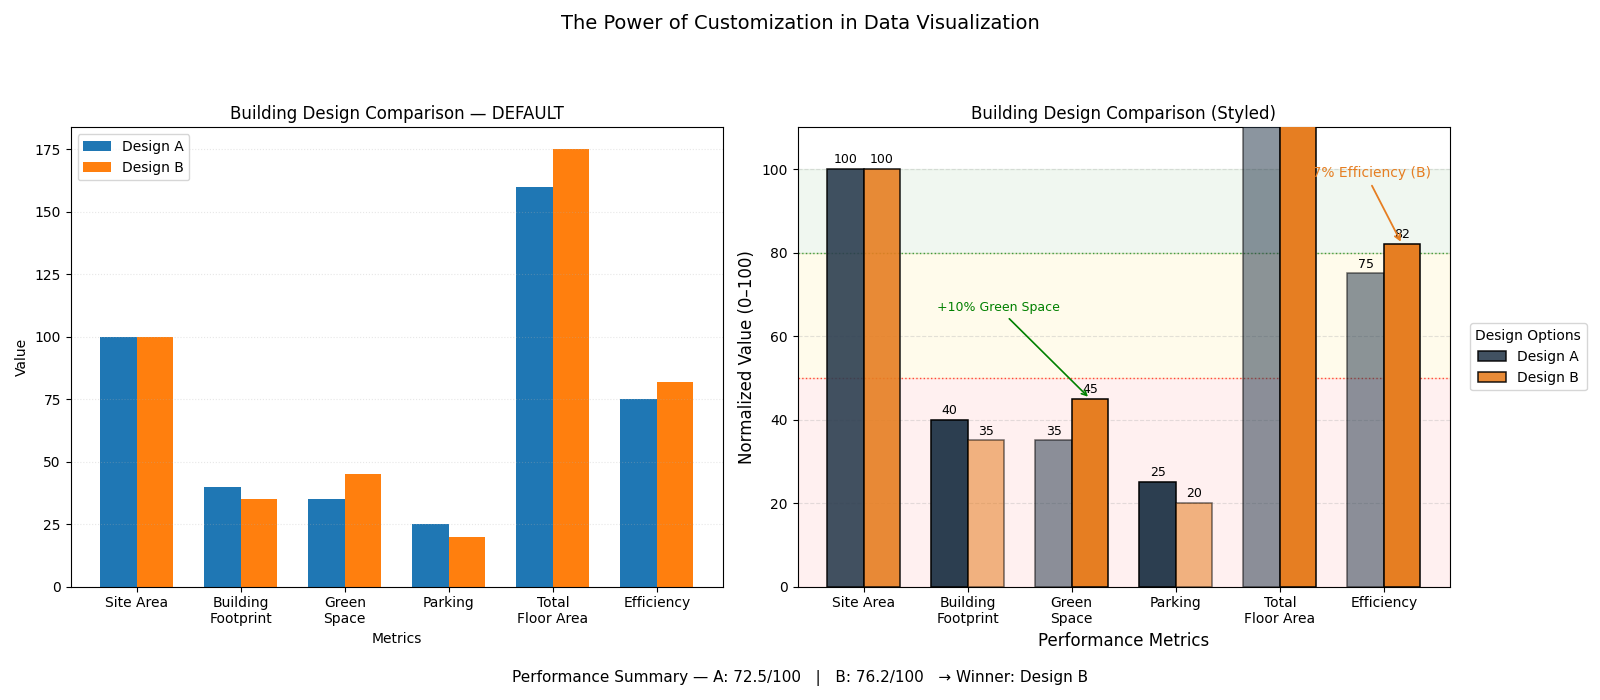
\includegraphics[width=\linewidth]{Figures/Visualization/16.11.png}
    \caption{Improved default vs.\ customized plots. Legends are placed outside, labels use real line breaks, and titles no longer overlap.}
    \label{fig:customization_v3}
\end{figure}


\hh{Colormap selection and layout refinement}

The gallery below (Figure~\ref{fig:colormap_v3}) demonstrates sequential, diverging, and qualitative colormaps with consistent margins and spacing. Tight layout ensures no title overlaps.

\code{c16_colormaps_detailed_v3}{python}{
    import numpy as np
    import matplotlib.pyplot as plt
    import matplotlib.cm as cm
    import matplotlib.colors as mcolors

    # Data fields
    x = np.linspace(-10, 10, 20)
    y = np.linspace(-10, 10, 20)
    X, Y = np.meshgrid(x, y)

    edge = np.minimum(np.minimum(np.abs(X-10), np.abs(X+10)),
                      np.minimum(np.abs(Y-10), np.abs(Y+10)))
    daylight = 8*np.exp(-edge/3) + np.random.random((20, 20))*0.4
    d_vmin, d_vmax = 0, 8
    temp = 3*(Y/10) + (np.random.random((20, 20))-0.5)*2
    t_norm = mcolors.TwoSlopeNorm(vmin=-4, vcenter=0.0, vmax=4)

    # --- Gallery (decluttered) ---
    fig, axes = plt.subplots(2, 3, figsize=(15, 8))
    items = [
        ('viridis',   'Sequential'),
        ('cividis',   'Sequential (CB-friendly)'),
        ('RdYlBu_r',  'Diverging'),
        ('coolwarm',  'Diverging'),
        ('tab10',     'Qualitative'),
        ('gray',      'Grayscale'),
    ]

    for ax, (cmap_name, label) in zip(axes.ravel(), items):
        if 'Diverging' in label:
            im = ax.imshow(temp, cmap=cmap_name, norm=t_norm,
                           extent=[-10,10,-10,10], aspect='equal')
            cbar_label = 'dTemp (deg C)'
        elif 'Qualitative' in label:
            cats = np.digitize(daylight, bins=np.linspace(d_vmin, d_vmax, 11)) - 1
            qmap = cm.get_cmap('tab10', 10)
            im = ax.imshow(cats, cmap=qmap, vmin=0, vmax=9,
                           extent=[-10,10,-10,10], aspect='equal')
            cbar_label = 'Zone'
        else:
            im = ax.imshow(daylight, cmap=cmap_name, vmin=d_vmin, vmax=d_vmax,
                           extent=[-10,10,-10,10], aspect='equal')
            cbar_label = 'Daylight Factor (%)'

        ax.set_title(f'{cmap_name} — {label}', fontsize=10, pad=4)
        ax.set_xticks([]); ax.set_yticks([])
        cbar = plt.colorbar(im, ax=ax, fraction=0.035, pad=0.02)
        cbar.set_label(cbar_label, fontsize=8)
        cbar.ax.tick_params(labelsize=8)

    fig.suptitle('Colormap Selection Gallery (Decluttered)', fontsize=13)
    plt.tight_layout(rect=[0, 0, 1, 0.95])
    plt.show()

    # --- Best practices (clean layout) ---
    fig2, axes2 = plt.subplots(2, 2, figsize=(12, 8))
    data = np.random.random((10, 8))*100
    for f in range(10):
        for b in range(8):
            data[f, b] += (f/10)*30 + (1 - abs(b-3.5)/3.5)*20

    im1 = axes2[0,0].imshow(data, cmap='YlOrRd', aspect='auto')
    axes2[0,0].set_title('GOOD: Sequential', color='green', fontsize=11, pad=4)
    plt.colorbar(im1, ax=axes2[0,0], fraction=0.05, pad=0.03)

    im2 = axes2[0,1].imshow(data, cmap='jet', aspect='auto')
    axes2[0,1].set_title('POOR: Rainbow (jet)', color='red', fontsize=11, pad=4)
    plt.colorbar(im2, ax=axes2[0,1], fraction=0.05, pad=0.03)

    im3 = axes2[1,0].imshow(data, cmap='cividis', aspect='auto')
    axes2[1,0].set_title('ACCESSIBLE: Cividis', color='green', fontsize=11, pad=4)
    plt.colorbar(im3, ax=axes2[1,0], fraction=0.05, pad=0.03)

    im4 = axes2[1,1].imshow(data, cmap='gray', aspect='auto')
    axes2[1,1].set_title('PRINT: Grayscale', color='green', fontsize=11, pad=4)
    plt.colorbar(im4, ax=axes2[1,1], fraction=0.05, pad=0.03)

    for ax in axes2.ravel():
        ax.set_xticks([])
        ax.set_yticks([])

    fig2.suptitle('Colormap Best Practices (Clean Layout)', fontsize=13)
    plt.tight_layout(rect=[0, 0, 1, 0.95])
    plt.show()
}{Colormap examples — decluttered layout with consistent margins and spacing.}

\begin{figure}[htp!]
    \centering
    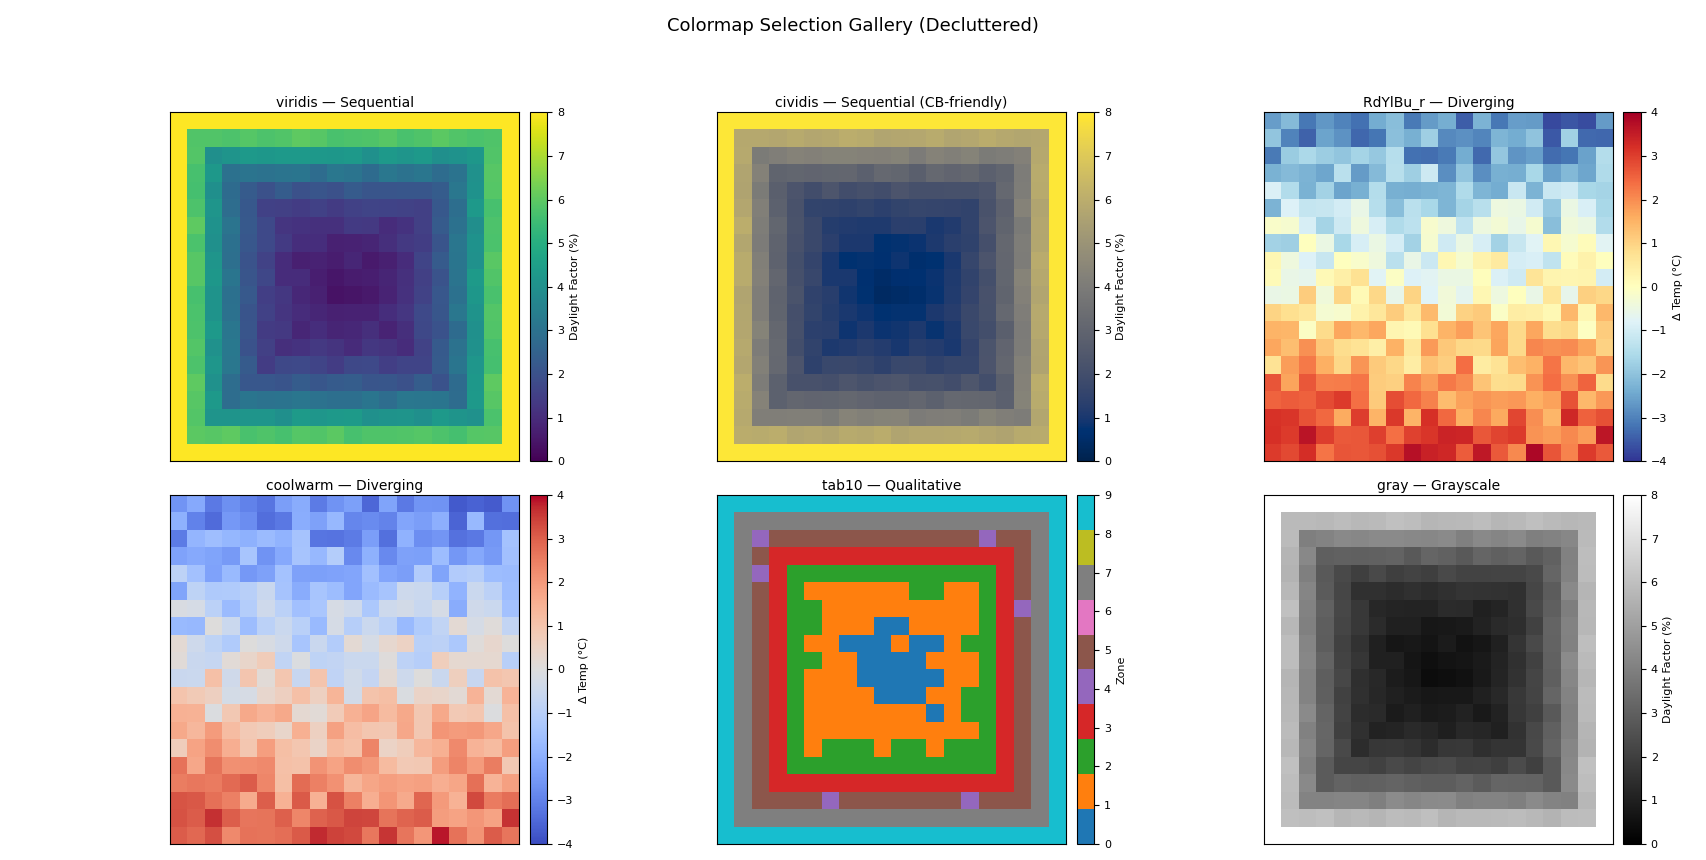
\includegraphics[width=\linewidth]{Figures/Visualization/16.12.png}
    \caption{Decluttered gallery of sequential, diverging, and qualitative colormaps. Titles and colorbars are evenly spaced, with tight layout preventing overlap.}
    \label{fig:colormap_v3}
\end{figure}

\section*{COLORMAP SELECTION GUIDELINES}

\begin{tcolorbox}[
  title=Colormap selection guidelines,
  colframe=blue,
  colback=white,
  arc=2mm,
  breakable
]
\textbf{1. Sequential colormaps (low $\rightarrow$ high)}\\
Use for: daylight levels, energy use, occupancy density.\\
Examples: \texttt{viridis}, \texttt{plasma}, \texttt{YlOrRd}, \texttt{Blues}.
\begin{itemize}
  \item Shows smooth progression clearly.
  \item Works in grayscale; good luminance ramp.
\end{itemize}

\medskip
\textbf{2. Diverging colormaps (deviation around a center)}\\
Use for: temperature variation, cost over/underruns, performance vs.\ target.\\
Examples: \texttt{RdYlBu}, \texttt{coolwarm}, \texttt{seismic}.
\begin{itemize}
  \item Emphasizes departure from a neutral midpoint.
  \item Make the zero/target value the center (use \texttt{TwoSlopeNorm}).
\end{itemize}

\medskip
\textbf{3. Qualitative colormaps (unordered categories)}\\
Use for: space types, material types, design options.\\
Examples: \texttt{tab10}, \texttt{Set1}, \texttt{Paired}.
\begin{itemize}
  \item Distinct hues per category.
  \item Do not imply numeric order or magnitude.
\end{itemize}

\medskip
\textbf{4. Avoid these common mistakes}
\begin{itemize}
  \item \textbf{Rainbow (\texttt{jet})}: introduces false boundaries and non-uniform contrast.
  \item \textbf{Red--green only}: not color-vision-friendly.
  \item \textbf{Too many colors}: hard to parse; group or label instead.
  \item \textbf{Low contrast}: unreadable in print or on projectors.
\end{itemize}

\medskip
\textbf{5. Accessibility considerations}
\begin{itemize}
  \item Test with a color-blind simulator or use color-blind-safe maps (e.g., \texttt{viridis}).
  \item Provide secondary encodings (patterns, markers, labels).
  \item Ensure sufficient contrast (check grayscale/photocopy).
  \item Consider grayscale printing; sequential maps should remain legible.
\end{itemize}

\medskip
\textbf{Quick rules of thumb}
\begin{itemize}
  \item Ratio data $\Rightarrow$ sequential; deviation from target/zero $\Rightarrow$ diverging; categories $\Rightarrow$ qualitative.
  \item Always label units and show a colorbar with ticks that mean something.
  \item Normalize data appropriately (min--max or centered around zero).
\end{itemize}
\end{tcolorbox}

% Optional: minimal Matplotlib examples (4-space indent as requested)
\code{c16_colormap_examples}{python}{
    import numpy as np
    import matplotlib.pyplot as plt
    from matplotlib.colors import TwoSlopeNorm
    from matplotlib import cm

    rng = np.random.default_rng(0)
    data_seq = rng.uniform(0, 100, size=(20, 30))          # sequential example
    data_div = rng.normal(loc=0, scale=1, size=(20, 30))   # diverging example
    cats = rng.integers(0, 10, size=(20, 30))              # qualitative example

    fig, axes = plt.subplots(1, 3, figsize=(12, 3))

    # 1) Sequential: viridis
    im0 = axes[0].imshow(data_seq, cmap='viridis', aspect='auto')
    axes[0].set_title('Sequential (viridis)')
    fig.colorbar(im0, ax=axes[0])

    # 2) Diverging: center at zero using TwoSlopeNorm + RdYlBu
    norm = TwoSlopeNorm(vmin=data_div.min(), vcenter=0.0, vmax=data_div.max())
    im1 = axes[1].imshow(data_div, cmap='RdYlBu', norm=norm, aspect='auto')
    axes[1].set_title('Diverging (centered at 0)')
    fig.colorbar(im1, ax=axes[1])

    # 3) Qualitative: 10 categories with tab10
    cmap_q = cm.get_cmap('tab10', 10)  # 10 distinct colors
    im2 = axes[2].imshow(cats, cmap=cmap_q, aspect='auto')
    axes[2].set_title('Qualitative (tab10)')
    cbar = fig.colorbar(im2, ax=axes[2], ticks=range(10))
    cbar.ax.set_ylabel('Category', rotation=270, labelpad=12)

    fig.tight_layout()
    plt.show()
}{Choosing colormaps: sequential for magnitudes, diverging for deviations, qualitative for categories}

\hhh{Common pitfalls and checklist}

\begin{itemize}
    \item \textbf{Wrong type}: don’t show deviations with a sequential map—use diverging centered at the neutral value.
    \item \textbf{Inconsistent ranges}: fix \texttt{vmin/vmax} across comparable figures; otherwise colors can’t be compared.
    \item \textbf{Rainbow (jet)}: avoid “jet”; it creates false edges and uneven contrast.
    \item \textbf{Accessibility}: prefer \texttt{viridis}/\texttt{cividis}; avoid red--green contrasts; verify grayscale legibility.
    \item \textbf{Too many hues}: for categories, cap at $\sim$6–10; beyond that, group or annotate.
    \item \textbf{Unclear legend}: always include a colorbar with interpretable ticks/units.
\end{itemize}


\hh{3D plots (mplot3d)}

3D plots are useful when geometry or scalar fields genuinely require depth (e.g., terrain, radiation domes, circulation paths). Figures~\ref{fig:three_d_line_scatter}–\ref{fig:three_d_bar} show the essential plot types with clean camera angles and compact colorbars to avoid clutter.

\begin{tcolorbox}[title=Getting a 3D axes (modern and legacy), colframe=blue, colback=white, arc=2mm, breakable]
\textbf{Modern:} create a 3D axes with \verb|subplot_kw={"projection": "3d"}| or \verb|fig.add_subplot(..., projection="3d")|.\\
\textbf{Legacy note:} older code sometimes imports \verb|Axes3D| from \verb|mpl_toolkits.mplot3d|. Keeping it is harmless.
\end{tcolorbox}

\hhh{3D line and scatter}

Use a continuous line for a trajectory and a sparse scatter for sample points. Figure~\ref{fig:three_d_line_scatter} shows a helix with a light tilt; \verb|set_box_aspect| keeps axes scales balanced.

\begin{tcolorbox}[title=Key syntax, colframe=blue, colback=white, arc=2mm, breakable]
\verb|ax.plot3D(x, y, z, **style)|  draws a 3D polyline. \quad
\verb|ax.scatter3D(x, y, z, s=..., **style)|  draws 3D markers.\\
\verb|ax.set(xlabel="x", ylabel="y", zlabel="z")|,\; \verb|ax.set_title("...")|,\; \verb|ax.view_init(elev, azim)|.
\end{tcolorbox}

\code{c16_3d_line_scatter}{python}{
    import numpy as np
    import matplotlib.pyplot as plt
    from mpl_toolkits.mplot3d import Axes3D  # legacy-safe (no effect on new versions)

    t = np.linspace(0, 4*np.pi, 200)
    x = np.cos(t); y = np.sin(t); z = t/(2*np.pi)

    fig, ax = plt.subplots(subplot_kw={"projection": "3d"}, figsize=(6, 4))
    ax.plot3D(x, y, z, lw=1.6, label="helix")
    ax.scatter3D(x[::10], y[::10], z[::10], s=20, color="C1", depthshade=False)
    ax.set(xlabel="x", ylabel="y", zlabel="z", title="3D line and scatter")
    ax.view_init(elev=25, azim=35)
    ax.set_box_aspect((1, 1, 1))
    ax.legend(loc="upper left")
    plt.tight_layout()
    plt.show()
}{3D line trajectory with sampled points.}

\begin{figure}[htp!]
    \centering
    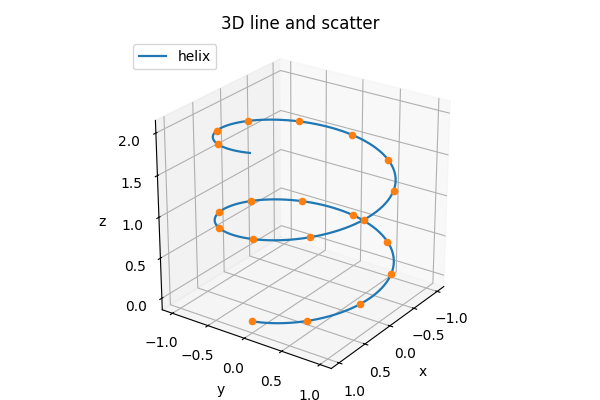
\includegraphics[width=0.6\linewidth]{Figures/Visualization/16.13.1.png}
    \caption{3D line and scatter on a helix. Balanced box aspect and a gentle tilt keep the scene readable.}
    \label{fig:three_d_line_scatter}
\end{figure}

\hhh{3D surface}

Surfaces communicate continuous scalar fields (e.g., terrain, pressure, radiation). Keep the colorbar narrow and the aspect ratio reasonable, as in Figure~\ref{fig:three_d_surface}.

\begin{tcolorbox}[title=Key syntax, colframe=blue, colback=white, arc=2mm, breakable]
\verb|X, Y = np.meshgrid(x, y, indexing="xy")| builds the grid. \quad
\verb|surf = ax.plot_surface(X, Y, Z, cmap=..., antialiased=True)|.\\
\verb|fig.colorbar(surf, ax=ax, shrink=..., pad=...)| attaches a compact colorbar.
\end{tcolorbox}

\code{c16_3d_surface}{python}{
    import numpy as np
    import matplotlib.pyplot as plt

    x = np.linspace(-3, 3, 120)
    y = np.linspace(-3, 3, 120)
    X, Y = np.meshgrid(x, y, indexing="xy")
    R = np.sqrt(X**2 + Y**2)
    Z = np.sin(R)

    fig, ax = plt.subplots(subplot_kw={"projection": "3d"}, figsize=(6, 4))
    surf = ax.plot_surface(X, Y, Z, cmap="viridis", linewidth=0, antialiased=True)
    cb = plt.colorbar(surf, ax=ax, shrink=0.75, pad=0.05)
    cb.set_label("value")
    ax.set(xlabel="x", ylabel="y", zlabel="z", title="3D surface")
    ax.view_init(30, 45)
    ax.set_box_aspect((1, 1, 0.6))
    plt.tight_layout()
    plt.show()
}{Smooth surface with compact colorbar.}

\begin{figure}[htp!]
    \centering
    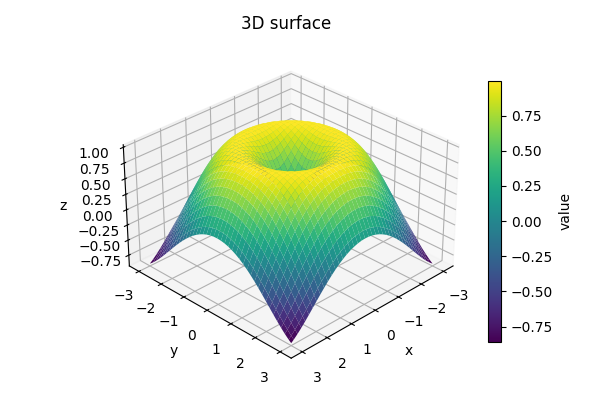
\includegraphics[width=0.6\linewidth]{Figures/Visualization/16.13.2.png}
    \caption{Radial sinusoid plotted as a surface. A slim colorbar and modest z aspect prevent clutter.}
    \label{fig:three_d_surface}
\end{figure}

\hhh{3D wire frame}

Wireframes emphasize shape without occluding interior regions. Increase strides to thin the grid (Figure~\ref{fig:three_d_wireframe}).

\begin{tcolorbox}[title=Key syntax, colframe=blue, colback=white, arc=2mm, breakable]
\verb|ax.plot_wireframe(X, Y, Z, rstride=..., cstride=..., color="...")|\\
Use strides to reduce line density for speed and clarity.
\end{tcolorbox}

\code{c16_3d_wireframe}{python}{
    import numpy as np
    import matplotlib.pyplot as plt

    x = np.linspace(-3, 3, 50)
    y = np.linspace(-3, 3, 50)
    X, Y = np.meshgrid(x, y, indexing="xy")
    Z = np.cos(X) * np.sin(Y)

    fig, ax = plt.subplots(subplot_kw={"projection": "3d"}, figsize=(6, 4))
    ax.plot_wireframe(X, Y, Z, rstride=2, cstride=2, color="gray")
    ax.set(xlabel="x", ylabel="y", zlabel="z", title="3D wireframe")
    ax.view_init(30, 40)
    ax.set_box_aspect((1, 1, 0.6))
    plt.tight_layout()
    plt.show()
}{Wireframe grid to reveal surface shape.}

\begin{figure}[htp!]
    \centering
    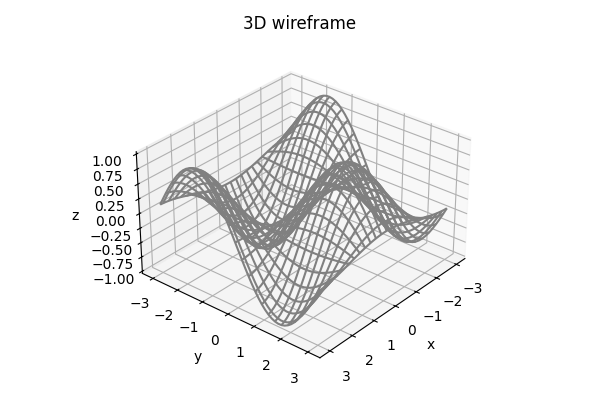
\includegraphics[width=0.6\linewidth]{Figures/Visualization/16.13.3.png}
    \caption{Wireframe of \(\cos x \sin y\). Thinned grid lines avoid the busy look common in 3D scenes.}
    \label{fig:three_d_wireframe}
\end{figure}

\hhh{3D contour}

3D contours highlight iso-values (e.g., thresholds or elevation lines). Keep the number of levels moderate and use a compact colorbar (Figure~\ref{fig:three_d_contour}).

\begin{tcolorbox}[title=Key syntax, colframe=blue, colback=white, arc=2mm, breakable]
\verb|ax.contour3D(X, Y, Z, levels=..., cmap=...)| \quad \verb|fig.colorbar(...)| for a legend.\\
Pick \verb|levels| deliberately to balance detail and clarity.
\end{tcolorbox}

\code{c16_3d_contour}{python}{
    import numpy as np
    import matplotlib.pyplot as plt

    x = np.linspace(-3, 3, 80)
    y = np.linspace(-3, 3, 80)
    X, Y = np.meshgrid(x, y, indexing="xy")
    Z = np.exp(-(X**2 + Y**2)) * np.cos(3*X) * np.sin(3*Y)

    fig, ax = plt.subplots(subplot_kw={"projection": "3d"}, figsize=(6, 4))
    cs = ax.contour3D(X, Y, Z, levels=25, cmap="plasma")
    cb = plt.colorbar(cs, ax=ax, shrink=0.75, pad=0.05)
    cb.set_label("value")
    ax.set(xlabel="x", ylabel="y", zlabel="z", title="3D contour")
    ax.view_init(35, -60)
    ax.set_box_aspect((1, 1, 0.6))
    plt.tight_layout()
    plt.show()
}{3D iso-value lines with legend.}

\begin{figure}[htp!]
    \centering
    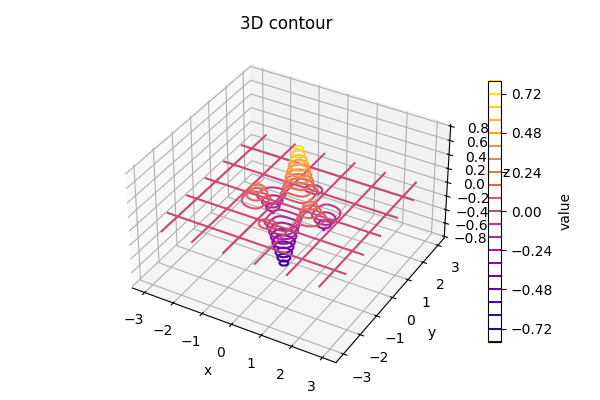
\includegraphics[width=0.6\linewidth]{Figures/Visualization/16.13.4.png}
    \caption{Iso-value lines for an oscillatory Gaussian. A small colorbar and limited levels keep the figure clean.}
    \label{fig:three_d_contour}
\end{figure}

\hhh{3D bar}

3D bars suit categorical values across a 2D grid (e.g., floor by unit). Keep the grid size modest and label axes clearly; see Figure~\ref{fig:three_d_bar}.

\begin{tcolorbox}[title=Key syntax, colframe=blue, colback=white, arc=2mm, breakable]
\verb|ax.bar3d(x, y, z, dx, dy, dz, shade=True)|. \quad
\verb|x,y| are bar bases; \verb|z| is the base height (often zeros); \verb|dx,dy,dz| are sizes.
\end{tcolorbox}

\code{c16_3d_bar}{python}{
    import numpy as np
    import matplotlib.pyplot as plt

    floors = np.arange(0, 4)   # 0..3
    units  = np.arange(0, 6)   # 0..5
    F, U = np.meshgrid(floors, units, indexing="ij")
    heights = 40 + 10*np.sin(F) + 5*np.cos(U)

    fig, ax = plt.subplots(subplot_kw={"projection": "3d"}, figsize=(6, 4))
    dx = dy = 0.8
    ax.bar3d(F.ravel(), U.ravel(), np.zeros(F.size),
             dx, dy, heights.ravel(), shade=True)
    ax.set(xlabel="Floor", ylabel="Unit", zlabel="Value", title="3D bar (floor x unit)")
    ax.view_init(25, 35)
    ax.set_box_aspect((1.2, 1, 0.6))
    plt.tight_layout()
    plt.show()
}{3D bars across a floor-by-unit grid.}

\begin{figure}[htp!]
    \centering
    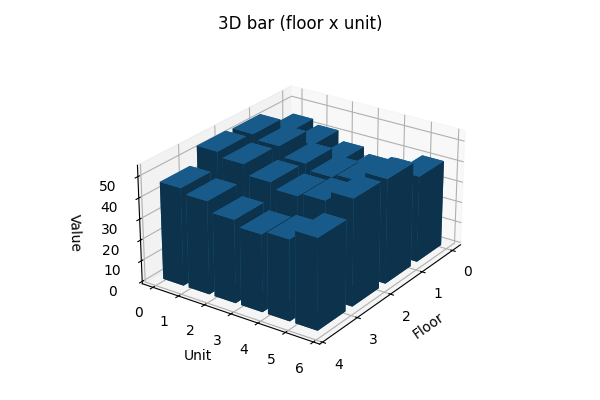
\includegraphics[width=0.6\linewidth]{Figures/Visualization/16.13.5.png}
    \caption{3D bar chart on a floor-by-unit grid. Limiting bar count and using a balanced aspect maintain legibility.}
    \label{fig:three_d_bar}
\end{figure}

\hh{3D plots — quick syntax recap}

\begin{tcolorbox}[title=3D plot syntax cheat-sheet, colframe=blue, colback=white, arc=2mm, breakable]
\textbf{Create 3D axes: } \verb|fig, ax = plt.subplots(subplot_kw={"projection": "3d"})| or \verb|ax = fig.add_subplot(111, projection="3d")|.\\
\textbf{Line \& scatter: } \verb|ax.plot3D(x,y,z, ...)|, \verb|ax.scatter3D(x,y,z, s=..., ...)|.\\
\textbf{Surface \& wireframe: } \verb|ax.plot_surface(X,Y,Z, cmap=..., ...)|, \verb|ax.plot_wireframe(X,Y,Z, rstride=..., cstride=...)|.\\
\textbf{Contours: } \verb|ax.contour3D(X,Y,Z, levels=..., cmap=...)|. \quad
\textbf{Bars: } \verb|ax.bar3d(x,y,z, dx,dy,dz, shade=True)|.\\
\textbf{Colorbar: } \verb|mappable = ax.plot_surface(...); fig.colorbar(mappable, ax=ax)|.\\
\textbf{View control: } \verb|ax.view_init(elev=..., azim=...)|; \verb|ax.set_box_aspect((1,1,1))| for equal scales.
\end{tcolorbox}

\hh{Common pitfalls and best practices}
\begin{itemize}
    \item \textbf{Grids for surfaces:} \verb|X|, \verb|Y|, \verb|Z| must be same 2D shape; build with \verb|np.meshgrid|.
    \item \textbf{Colorbars:} keep them tied to the returned mappable (e.g., from \verb|plot_surface|).
    \item \textbf{View \& aspect:} use \verb|ax.view_init(elev, azim)| and \verb|ax.set_box_aspect((1,1,1))| for equal axes.
    \item \textbf{Subplots:} create each 3D Axes with \verb|projection='3d'| via \verb|add_subplot| or \verb|subplots(..., subplot_kw=...)|.
\item \textbf{Performance:} dense surfaces are heavy; reduce resolution or use wireframe while exploring.
\end{itemize}

% =====================
% KEY TAKEAWAYS
% =====================

\hh{Key takeaways}

\begin{tcolorbox}[
    colframe=orange,
    colback=white,
    arc=2mm
]
\begin{itemize}
    \item \textbf{Start simple}: Begin with basic plots and gradually add complexity
    \item \textbf{Always label}: Include units (m2, kWh, C), axis labels, titles, and legends
    \item \textbf{Choose wisely}: Bar for categories, line for time, scatter for relationships
    \item \textbf{Color purposefully}: Use color to encode information, not just for decoration
    \item \textbf{Annotate insights}: Point out key findings directly on the plot
    \item \textbf{Check your data}: Visualizations can reveal data quality issues
    \item \textbf{Export appropriately}: PNG for presentations (300 DPI), PDF for reports (vector)
\end{itemize}
\end{tcolorbox}
